\chapter{The ATLAS Trigger System}
\label{sec:trig}

In 2015 and 2016, the LHC has been colliding proton bunches every \SI{25}{\nano\second},
meaning that the ATLAS experiment has been collecting data at a rate of 40 MHz.
Due to the large computing resources required to process and store each event,
it is not possible to record all events.
The most interesting events to study contain a hard-scatter collision,
defined as a collision in which the momentum transfer is large compared to the proton mass~\cite{trig-hard_scatter},
as these are the collisions that, for example, can produce a TeV scale BSM particle.
Therefore, the ATLAS experiment uses a trigger system to select events that contain
contain a high-$p_{T}$ physics object which indicates that a hard-scatter collision has occurred.

The ATLAS trigger-system consists of two levels;
the first level trigger (L1) and the higher level trigger (HLT)~\cite{det-run2_trigger}.
Figure~\ref{fig:det-trigger_schem} shows a schematic outlining the trigger system used in Run-2
\footnote{\ The period of data-taking starting in 2015 and scheduled to continue until the end 2018 is known as Run-2.}~\cite{det-run2_triggerPerf}. 

The L1 trigger is hardware based and reduces the rate from 40~MHz to 100~kHz within a time window of \SI{2.2}{\micro\second}.
The L1 trigger uses custom electronics to rapidly process information directly from the
calorimeter and Muon Spectrometer, searching for high-$p_{T}$ muon tracks and large energy deposits in the calorimeter.
The central trigger processor then uses a set of pre-defined conditions
to decide if a L1 trigger accept is given. 
At the same time Regions of Interests (RoIs) are constructed around the high-\pT{} objects identified by the L1 trigger, which are utilised by the HLT. 

If the L1 trigger is passed the event is processed by the HLT,
%The next step is the HLT,
a software based trigger,
which further reduces the event rate to 1~kHz within a time window of ~\SI{0.2}{\second}.
The HLT uses the information from the full detector
to perform a more complete reconstruction of the physics objects within the event,
the most time consuming reconstruction algorithms only being run only within the RoIs taken from L1.
The more complex event analysis within the software-based trigger includes
track reconstruction and therefore allows for $b$-jet identification.
If the content of the event reconstruction passes a pre-set criteria, a HLT accept is issued
meaning that the events are passed on for processing and storage. 
% in offline computer farms (known as tier-0).

\begin{figure}[!htb]
  \begin{center}
    \includegraphics[width=0.75\linewidth, angle=0]{figs/Detector/trigger_schem.png}
  \end{center}
  \vspace{-1em}
  \caption[A schematic of the ATLAS trigger and data-acquisition system in Run-2, with a focus on the components required for triggering.]
          {A schematic of the ATLAS trigger and data-acquisition system in Run-2, with a focus on the components required for triggering~\cite{det-run2_triggerPerf}.}
  \label{fig:det-trigger_schem}
\end{figure}

In the ATLAS trigger system there is an additional process known as pre-scaling that can be applied.
If a trigger is pre-scaled, only a fraction of the events that pass the trigger are recorded.
Pre-scaling is applied to maintain the output rate of the L1 and HLT trigger systems at 100 and 1~kHz respectively as the instantaneous luminosity of the LHC collisions is increased.
An unprescaled trigger is defined as a trigger that has no pre-scale applied to it.
Most analyses at ATLAS use unprescaled triggers to maximise the acceptance of the trigger.

%In the di-$b$-jet searches presented in this thesis, two different trigger strategies are used.
%A single jet trigger is used for the high-mass di-$b$-jet search and a double $b$-jet trigger for the low-mass di-$b$-jet search.
This chapter describes triggers used in the two di-$b$-jet searches presented in this thesis.
Section~\ref{sec:trig-jet} describes jet triggers used in the high-mass di-$b$-jet search,
Section~\ref{sec:trig-bjet} describes $b$-jet triggers  used in the low-mass di-$b$-jet search
and finally Section~\ref{sec:trig-bjet_eff} presents the measurement of the $b$-jet trigger efficiency, an essential input to the low-mass search.

There are two important definitions used in this chapter, and throughout this thesis.
\textit{`Online'} refers to any algorithms run or objects reconstructed at the trigger level.
\textit{`Offline'} refers to algorithms run after events have passed the trigger at the data-processing level.
Offline algorithms and objects used in this thesis are described in Chapter~\ref{sec:obj}.

\section{Jet Triggers}
\label{sec:trig-jet}

Section~\ref{sec:obj-jets} described that hadronic jets are built from energy deposits in the ATLAS calorimeter.
Jet triggers are tasked with selecting events that contain with one or more high-\pT{} jets,
which is challenging at hadron colliders due to the extremely high cross-sections of hadronic jet production.
In Run-2 the jet triggers are used at both the L1 and HLT level~\cite{trig-run2_proc}.

%\subsection{Level 1}

The L1 trigger is a hardware based trigger which accepts or rejects an event within \SI{2.2}{\micro\second}.
Due to this time constraint, the L1 jet trigger uses coarser jet reconstruction techniques than are used by offline reconstruction.
The L1 jet trigger uses trigger towers which are defined as energy deposits in a region of 0.1 x 0.1 in the $\eta-\phi$ plane integrated radially over all layers of the EM and hadronic calorimeter.
The L1 jet trigger accepts an event if a neighbouring group of 4x4 trigger towers containing energy deposits above some pre-set threshold is found.
%The di-$b$-jet searches use the L1 trigger known as \verb|L1_J100|, which requires that at least one trigger tower group with an energy deposit of \SI{100}{\GeV} has been found.
%Other L1 triggers that search for multiple clusters are also possible to reduce the energy thresholds required.
%The L1 trigger then seeds the HLT trigger.

In the  L1 trigger there is no tracking information, meaning that electron and taus
are also triggered on using similar techniques as hadronic jet algorithms, except using narrower groups of trigger towers.
In addition the $b$-jet triggers described in the following section are also seeded by an L1 jet trigger.

%\subsection{HLT}

The HLT jet trigger is able to use more complex algorithms to reconstruct jets due to the larger time allowed for a trigger decision.
Similar to offline jet reconstruction, in the HLT jets are reconstructed using 
hadronic topoclusters formed from EM or hadronic calorimeter cells and the anti-$k_T$ jet-reconstruction algorithm with $R$=0.4;
topoclusters and the anti-$k_T$ algorithms are described in Section~\ref{sec:obj-jets}.
The HLT jet trigger is passed if the reconstructed jets meet a pre-set criteria that depends on the number and $p_T$ of the jets.

%\subsection{High-mass trigger selection}

For the high-mass di-$b$-jet search the \verb|HLT_j380| trigger is used, which requires that at least one jet is found with a $p_T >$ 380 GeV.
This is chosen as it is the unprescaled single jet trigger with the lowest cut on jet-\pT{} in 2016 data-taking.
%meaning that of triggers that accept every event passing a single jet criteria,
%this trigger has the lowest jet-$p_T$ threshold.
%Due to the exponential increase in jet production cross-section at low jet-$p_T$,
%the $p_T$ threshold is set to keep the acceptance rates low enough such that the HLT trigger is within its output rate budget of 1~kHz.

However, as will be shown in Section~\ref{sec:evt},
the online jet $p_T$ threshold limits the mass region that the high-mass di-$b$-jet can probe to $m > 1.1$~TeV.
In the mass region $m < 1.1$~TeV a kinematic bias from the online jet $p_T$ threshold is introduced
such that the backgrounds from the Standard Model cannot be modelled. 
Therefore, for a di-$b$-jet search to probe lower masses a different trigger strategy is required.

\vfill

\section{$b$-Jet Triggers}
\label{sec:trig-bjet}

As described in Section~\ref{sec:obj-bjets}, $b$-jets, defined as jets containing a $b$-hadron,
can be identified from the topology of tracks in a process known as $b$-tagging.
$b$-Tagging can be utilised online to reduce rates of jets significantly~\footnote{\ As described in Section~\ref{sec:theo-qcd-dijet_features},
  the QCD dijet production is dominated by light-jets}
allowing for a lower jet-$p_T$ threshold than is used by the single jet trigger.
Hence, using a $b$-jet trigger in di-$b$-jet searches means that a lower mass range can be probed.
%$b$-Jet triggers have been used previous ATLAS analyses,
%for example searches for exotic particles decaying to 4 $b$-jets via a pair of Higgs bosons~\cite{trig-H4b}.

The $b$-jet trigger utilises the regions of interest (RoI) defined by the jets reconstructed in the L1 jet trigger.
The $b$-jet trigger procedure for 2016 data-taking contains three steps~\cite{trig-bTrig_desc}.
Firstly, a `fast'-tracking algorithm is run in the the RoIs and
%is run in a super-RoI,
%which is a superset of all RoIs which correspond to a L1 jet with $\pT{} >$ 30 GeV.
the reconstructed tracks are used to identify the hard-scatter primary vertex (PV) in the event.
Secondly, within each jet RoI precision tracking is run.
Finally, the precision tracks are used by the MV2 $b$-tagging algorithm, described in Section~\ref{sec:obj-bjets_MV2}, to identify $b$-jets.

Figure~\ref{fig:trig-bTrig_perf} shows the $b$-jet efficiency against light-jet and $c$-jet rejection \footnote{\ $b$-jet efficiency and
  light/$c$-jet rejection are defined in Section~\ref{sec:obj-bjets_MV2}}
for online $b$-tagging in a variety of $b$-jet trigger configurations in simulated $t\bar{t}$ events.
The black line represents the MV2c20 algorithm used in 2016 data-taking as described in Section~\ref{sec:obj-bjets_MV2}.
The blue line represents the IP3D+SV1 algorithm that combines two of the base $b$-tagging algorithms described in Section~\ref{sec:obj-bjets}.
IP3D+SV1 was used by the $b$-jet trigger in 2015 data-taking.

\begin{figure}[!ht]
  \begin{center}
    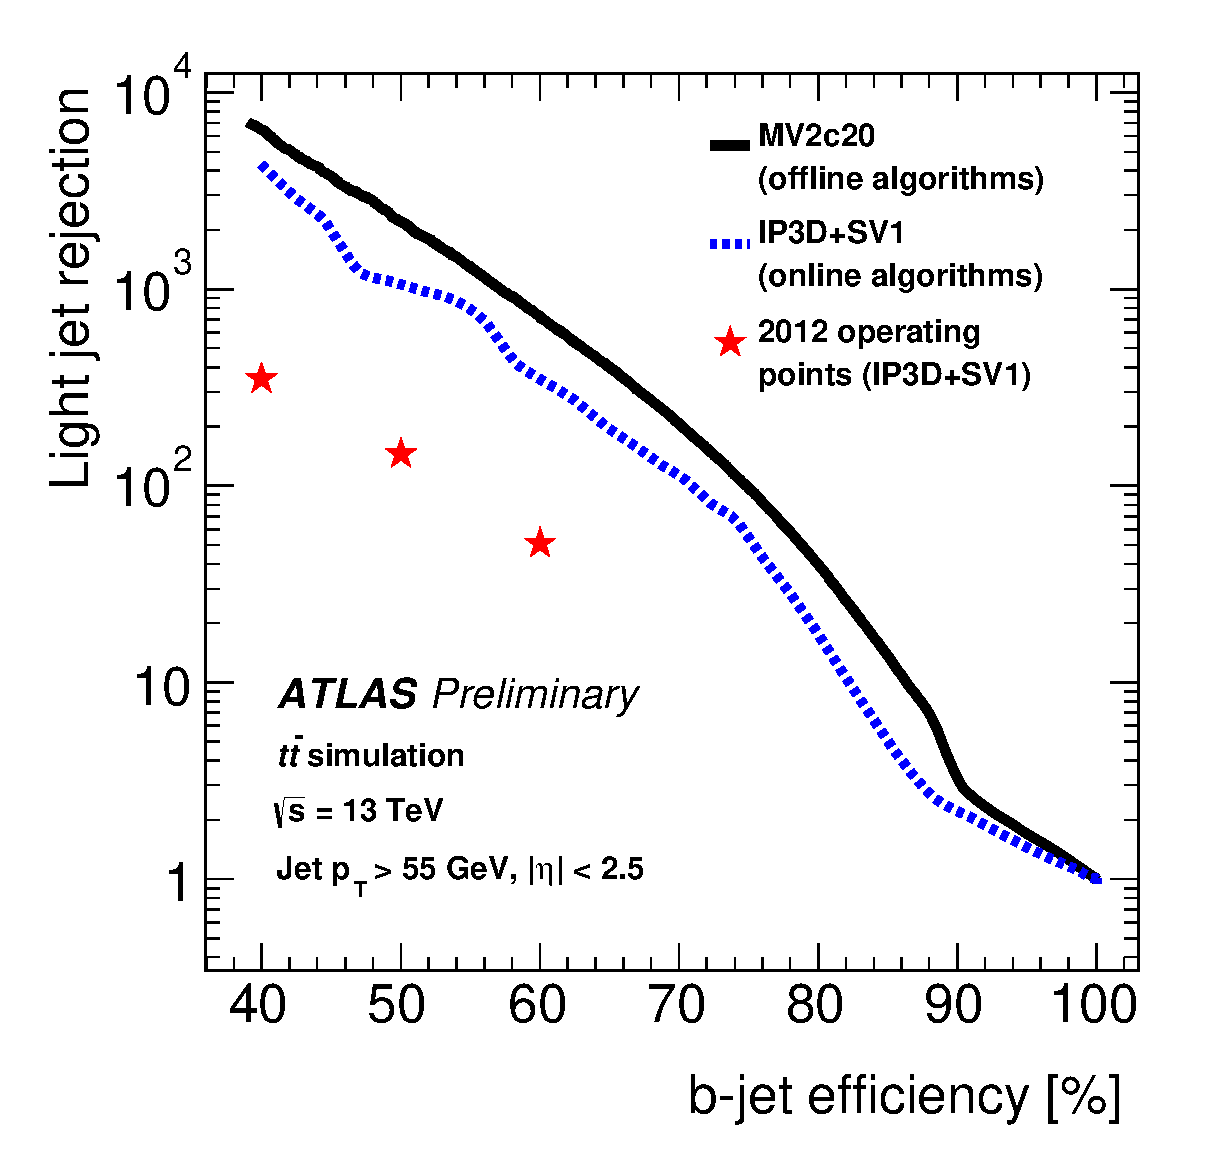
\includegraphics[width=0.48\linewidth, angle=0]{figs/Trigger/trig-bTrig_perf_light.eps}
    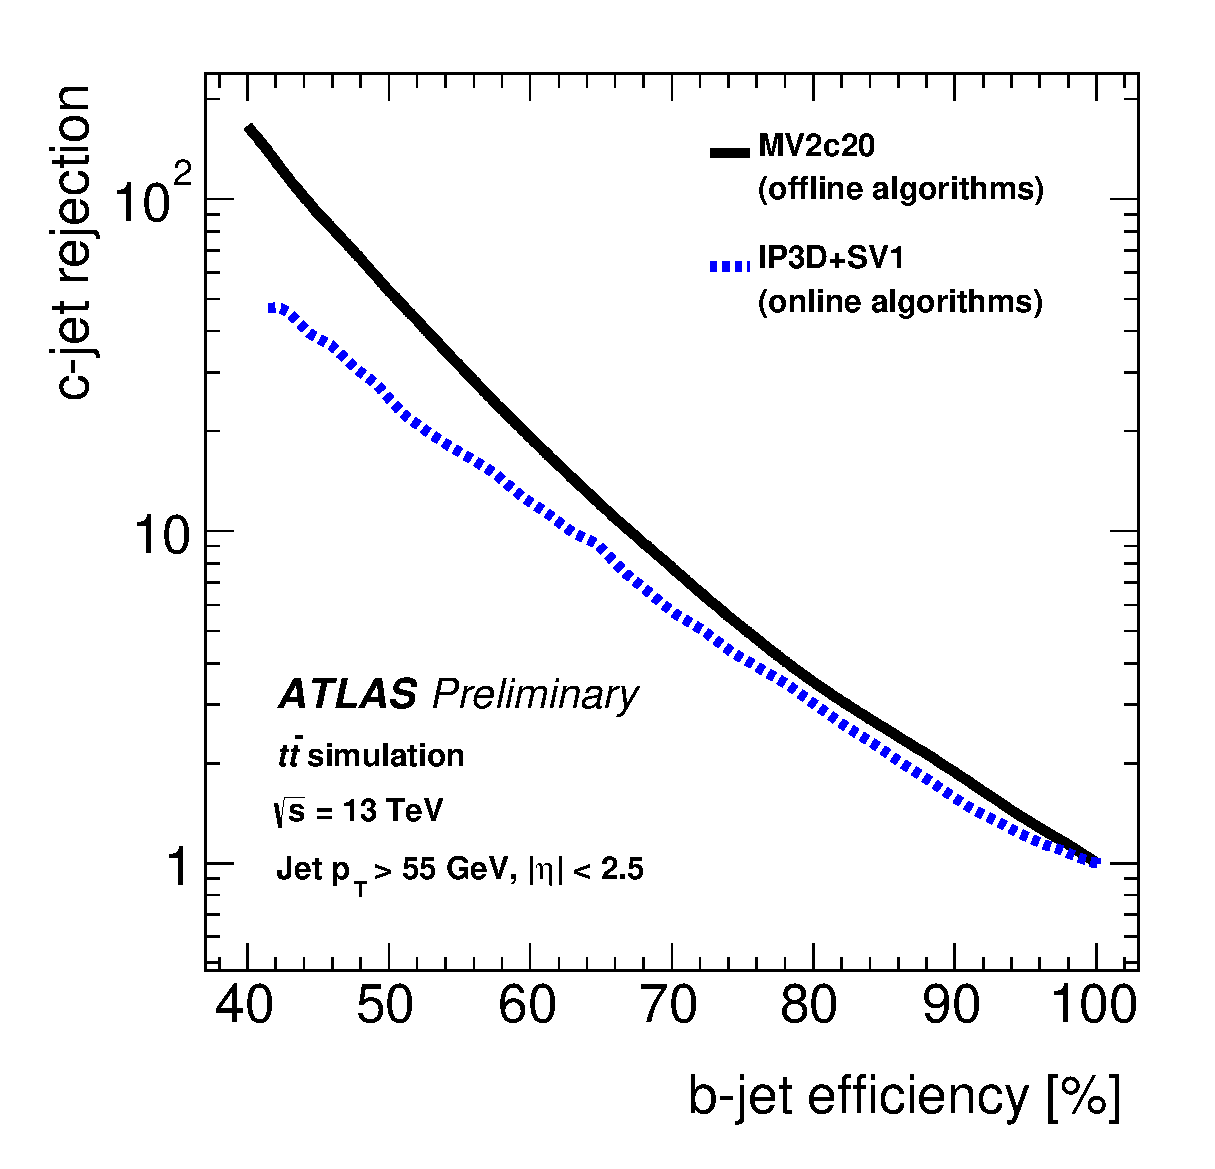
\includegraphics[width=0.48\linewidth, angle=0]{figs/Trigger/trig-bTrig_perf_charm.eps}
  \end{center}
  \caption[The expected $b$-jet efficiency of $b$-jet triggers in Run-2 compared to the set-up used in 2012 data-taking.]
    {The expected $b$-jet efficiency of $b$-jet triggers with respect to (a) light-jet and (b) $c$-jet rejection
    in the case where the $b$-tagging algorithm used is MV2c20 (black), IP3D+SV1 (blue) and for the set-up used in 2012 data-taking (red stars)~\cite{trig-bTrig_desc}.}
  \label{fig:trig-bTrig_perf}
\end{figure}


There are several $b$-jet triggers available
with a variety of requirements on the jet multiplicity, number of tagged jets and $b$-tag operating point used.
As the signal considered in the low mass di-$b$-jet search is a BSM particle decaying to two $b$-quarks, a double $b$-jet trigger is used.
The double $b$-jet trigger requires that there are two online jets with $p_T >$ 150 and 50 GeV respectively,
which have been $b$-tagged at the 60\% efficiency operating point~\footnote{The trigger is known as \textit{HLT\_j150\_bmv2c2060\_split\_j50\_bmv2c2060\_split}.}.
It will be shown in Chapter~\ref{sec:evt} that the low mass di-$b$-jet search is able to probe the mass range $m >$ 0.57 TeV.

There are significant differences in the  $b$-jet trigger configurations used in 2016 and 2015 data-taking.
Firstly, the online $b$-tagging algorithm is MV2c20 in 2016 data-taking whilst IP3D+SV1 was used in 2015 data-taking.
MV2c20 is used in 2016 due to improved $b$-tagging performance, as shown in Figure~\ref{fig:trig-bTrig_perf}.
Secondly, different algorithms are used to identify the hard-scatter primary vertex in 2015 and 2016 data.
2016 data-taking employs the \verb|xPrmVtx| algorithm, which is based on the hard-scatter primary vertex finding algorithm used offline, as described in Section~\ref{sec:obj-tracks_pv}.
In 2015 data-taking the \verb|EFHist| algorithm is employed~\cite{trig-EFHist};
which groups all tracks in a histogram based on the $z$ position of the track intersection with the beam-pipe,
and uses the centre of the bin containing the largest sum of track-\pT{} as the hard-scatter primary vertex.
%The \verb|xPrmVtx| algorithm is used in 2016 to align with offline tracking.
As a result of these significant differences, data taken in 2015 and 2016 by the $b$-jet trigger are not easily combined in a di-$b$-jet search.
Therefore, as described in Chapter~\ref{sec:evt}, the low mass di-$b$-jet search presented in this thesis uses only the 2016 data-set.

In addition there are important differences between online and offline $b$-tagging.
Firstly, coarser tracking information is available online, notably online tracks are only reconstructed within the jet RoIs.
Secondly, a different fraction of $c$-jets were present in the sample used to train the MV2 algorithm in online and offline $b$-tagging,
specifically 10\% were used offline (MV2c10) and 20\% were used online (MV2c20).
The training samples used by the MV2 algorithm are discussed in Section~\ref{sec:obj-bjets_MV2}.
The reason MV2c20 is used online in 2016 data-taking is that the $b$-jet trigger configuration
had to be determined before the start of data-taking in March 2016,
whilst the recommendation to use MV2c10 was announced internally in May 2016~\cite{obj-bjets_algo_2016}.
As offline and online $b$-tagging are significantly different, online $b$-tagging must have an independent calibration, which is described in the following section.


\section{ Measurement of the $b$-Jet Trigger Efficiency in 2016 Data}
\label{sec:trig-bjet_eff}

The trigger is critical in the event selection of any analysis,
therefore the performance of the triggers utilised must be understood and calibrated.
This section describes the \mbox{$b$-jet} trigger efficiency measurement in 2016 data,
which is an important input to the low-mass di-$b$-jet search presented in this thesis.

%\subsection{Strategy}
%\label{sec:trig-bjet_strat}

The $b$-jet trigger is always used in tandem with offline $b$-tagging, which is calibrated independently of the $b$-jet trigger, as described in Section~\ref{sec:obj-bjets_calib}.
%As mentioned before, there are many differences between offline and online $b$-tagging.
Therefore, the $b$-jet trigger efficiency, $\epsilon_{b\text{Trig}}$, is defined with respect to offline $b$-tagging;
specifically, $\epsilon_{b\text{Trig}}$ is defined as the number of $b$-jets that are offline $b$-tagged and match an online $b$-tagged trigger-jet
divided by the number of $b$-jets that are offline $b$-tagged and match a trigger jet.
Or to put this in an equation;
\begin{equation}
  \epsilon_{b\text{Trig}} = \frac{N(\text{Offline-tagged, online-tagged, $b$-jets)}}{N(\text{Offline-tagged, trigger-matched, $b$-jets)}}
  \label{eq:trig-eff}
\end{equation}
A $b$-jet is defined as a jet containing a $b$-hadron.
The process used to match trigger jets and offline jets is described in Section~\ref{sec:trig-evtSel}.
%$\epsilon_{b\text{Trig}}$ is probability if a $b$-jet is produced in a proton collitions,
%the jet will be $b$-tagged at the online level given that it created jet at the trigger level and that it would be $b$-tagged offline.

%As is done for offline $b$-tagging, as described in Section,
The $b$-jet trigger efficiency is measured in both data and Monte-Carlo simulated samples.
Then a $b$-jet trigger data/simulation scale factor ($SF_{\,b\text{Trig}}$), is derived, where:
\begin{equation}
 SF_{\,b\text{Trig}} = \epsilon_{\,b\text{Trig}}^{\text{Data}}/\epsilon_{\,b\text{Trig}}^{\text{Simulation}}
\end{equation}
The data/simulation scale-factor is applied to Monte-Carlo simulation to correct for mismodelling of the $b$-jet trigger performance.
The scale-factors for the $b$-jet trigger are to be applied in addition to the offline $b$-tagging scale factors described in Section~\ref{sec:obj-bjets_calib}.

%The data-sets, simulated samples and event selection used for the measurement of $b$-jet trigger efficiency are described below.
The $b$-jet trigger efficiency and data/simulation scale factors are measured for all combinations of offline and online $b$-tagging operating points.
Only the 70\% offline and 60\% online operating point combination is presented in this section,
as this is set of operating points used in the low mass di-$b$-jet search;
Chapter~\ref{sec:evt} contains full details of the $b$-tagging operating points used in di-$b$-jet searches.

%\newpage
\subsection{Description of Event Selection and Data-sets}
\label{sec:trig-evtSel}

Di-lepton $t\bar{t}$ events containing a muon and an electron are selected to provide a high purity sample of $b$-jets to measure the $b$-jet trigger efficiency.
As discussed in Section~\ref{sec:theo-ttbar}, 
$e\mu$ di-lepton $t\bar{t}$ events provide a distinctive signature for selection and a pure sample of $b$-jets required for the efficiency measurement.
Furthermore, the electron and muon provide a signature that can be used to select events at the trigger-level without using a $b$-jet trigger
such that no bias is introduced from online $b$-tagging.

\noindent
Specifically, events are required to:
\vspace{-1em}
\begin{itemize}
\item Pass one of two single lepton $b$-performance triggers that require
    \begin{itemize}[label={$-$}]
    \item An online reconstructed medium muon with $\pT >$ 26 GeV.
    \item Or an online reconstructed electron with $\pT >$ 26 GeV \footnote{The triggers are called \textit{HLT\_mu26\_imedium\_2j35\_bperf} and \textit{HLT\_e26\_tight\_iloose\_2j35\_bperf}.}.
    \end{itemize}
\item Contain an offline medium muon with $\pT>30~\GeV$ and no jet within $\Delta R$ of 0.4.
\item Contain an offline medium electron with $\pT>30~\GeV$.
\item Contain $\geq$ 2 offline $b$-tagged jets, defined as:
   \begin{itemize}[label={$-$}]
     \item Offline R=0.4 anti-$k_T$ jets.
     \item $\pT>35~\GeV$ and $|\eta|<2.5$.
     \item Offline $b$-tagged at the 85\%~operating point.
     \item The offline jet must be matched to an online jet.
    \end{itemize}
\end{itemize}
Details of muon, electron, jet and $b$-tagged jet object definition are in Chapter~\ref{sec:obj}.
%chapter ~\ref{sec:obj-lepton},~\ref{sec:obj-jets} and \ref{sec:obj-bjets}\textit{(sec:obj-bjet)} respectively.

The triggers deployed are $b$-performance triggers, which are special triggers used in data-taking specifically for monitoring the $b$-jet trigger performance.
They require that an online muon or an electron with $\pT{} > 26$~\GeV~is reconstructed.
The $b$-performance triggers then run the online $b$-tagging algorithms on all trigger jets with $|\eta|<2.5$ and
\mbox{$p_{T}>35$~\GeV} without performing any cuts on the output of the MV2c20 algorithm.
Therefore, $b$-performance triggers can select  di-lepton $t\bar{t}$ events at the trigger-level
and thus provide an unbiased source of online $b$-tagged jets to measure the $b$-jet trigger efficiency.

The leptons are required to have a $\pT >$ 30 GeV such that there is no kinematic bias from the online lepton $\pT$ requirement. 
The muon used for event selection is required to have no jet within  $\Delta R$ of 0.4 to exclude %fake $e\mu$ di-lepton $t\bar{t}$
events where the only muon is caused by the decay of the $b$-hadron within a $b$-jet, which would increase the fraction of non-$t\bar{t}$ backgrounds.

Offline jets are matched to online jets if $\Delta R < 0.4$,
the matching is exclusive meaning that online jets are only matched to offline jets with the smallest $\Delta R$ separation.
Matching is required such that the $b$-jet trigger efficiency measurement does not have a kinematic bias
from the online jet-$\pT$ requirement used in the $b$-performance trigger.
The 85\% operating point is chosen for offline $b$-tagging as an event selection with a tighter event selection
cannot be used to calibrate the 85\% operating point.



%this event selection is used to calibrate all offline operating points.
%A similar requirement on electrons is not applied as it is found that this has a negligible effect on the $b$-jet trigger efficiency
%and reduced stats at high pT, probably due to boosted topologies:
% To summarise:
% No overlap - bad data/simu agreement.
% E and mu overlap - better data/simu agreement, low stats at high pT, low purity at high pT
% mu overlap - good data/simu agreement, ok stats at high pT, high purity at high pT => Best option!!!



The data-set used is 13~TeV $pp$ collision data collected by the ATLAS detector between March and December 2016;
the same data-set is used by the low mass di-$b$-jet search presented in this thesis. %, which is discussed in Chapter~\ref{sec:evt}.
A $b$-jet trigger aware Good Run List (GRL) 
\footnote{A GRL is effectively a list of lumi-blocks that pass certain data-quality requirements.
  A further discussion of GRLs are found in Section~\ref{sec:evt-datasets}.}
is applied, Section~\ref{sec:trig-grl} describes the GRL and the motivations for its use.
After the application of the GRL the data-set corresponds to an integrated luminosity of 24.3~\ifb.

Events that pass an $e\mu$ di-lepton $t\bar{t}$ selection with 2 $b$-tags
are dominated by $t\bar{t}$ production with a small contribution from single-top production~\cite{trig-ttbar};
the remaining backgrounds are negligible and are not considered in this efficiency measurement.
For the simulated sample; a Monte-Carlo simulated $t\bar{t}$ sample is produced using the
Powheg-Box v2~\cite{trig-powheg} generator with the CT10 PDF sets~\cite{trig-CT10} in the matrix element calculations.
For the simulated single-top sample electro-weak t-channel, s-channel and $Wt$-channel single top-quark events are generated using the Powheg-Box v1 generator and CT10 PDF sets.
%This generator uses the 4-flavour scheme for the NLO matrix elements calculations together with the fixed four-flavour PDF
%For all top processes, top-quark spin correlations are preserved (for t-channel, top quarks are decayed using MadSpin[10a]).
For both processes the parton shower, fragmentation and the underlying event are simulated using Pythia6.428~\cite{trig-pythia6} with the CTEQ6L1~\cite{trig-CTEQ6L1} PDF sets
and the corresponding Perugia 2012 tune~\cite{trig-perugia}.
The top mass is set to 172.5 GeV.
The EvtGen v1.2.0 program~\cite{trig-evtGen} is used to model the decays of $b$ and $c$ hadrons.

\subsection{Investigation of Data-Simulation Discrepancies}
\label{sec:trig-inv}

This section will present the initial observation and investigation of discrepancies between the $b$-jet trigger efficiency measured in 2016 data and simulation.
%and the investigation into the discrepancies.
%The results of the studies in this section will be used in Section~\ref{sec:trig-grl} to describe the solution that has been implamented. 
To replicate the event selection used during the discrepancy and investigation studies the $b$-jet trigger aware GRL is not applied in this section.
%Otherwise the event selection used is indentical to the event selection described in~\ref{sec:trig-evtSel}.
%except that no .%, the triggers %are single lepton triggers without the additional $b$-performance functionality
%\footnote{\ Specifically HLT\_mu26\_imedium and HLT\_e26\_tight\_iloose.}
%and the offline jets are not required to match a trigger jet to be included in the denominator of $b$-jet trigger efficiency calculation.
%Furthermore, for reasons of simplicity, only $t\bar{t}$ events are included in the simulated sample during the investigation studies.
%Hence, throughout this section simulation refers to $t\bar{t}$ events only.
%In Section~\ref{sec:trig-cross-checks} it will be shown that the effect of single-top production is small
%and would not affect the conclusions of the investigation studies.

Figure~\ref{fig:trig-Full_noGRL_eff_noHLTMatch} shows the measured $b$-jet trigger efficiency in data and simulation against jet-\pT{} and $\eta$.
To accurately reflect the total $b$-jet trigger efficiency, %before the $b$-jet trigger GRL is applied
offline jets are not required to match online jets in the denominator of the $b$-jet trigger efficiency for this figure.
The reason for relaxing this requirement is described later in this section.

\begin{figure}[!htb]
  \begin{center}
    \captionsetup[subfigure]{aboveskip=0pt,justification=centering}
    \subcaptionbox{Jet-\pT}{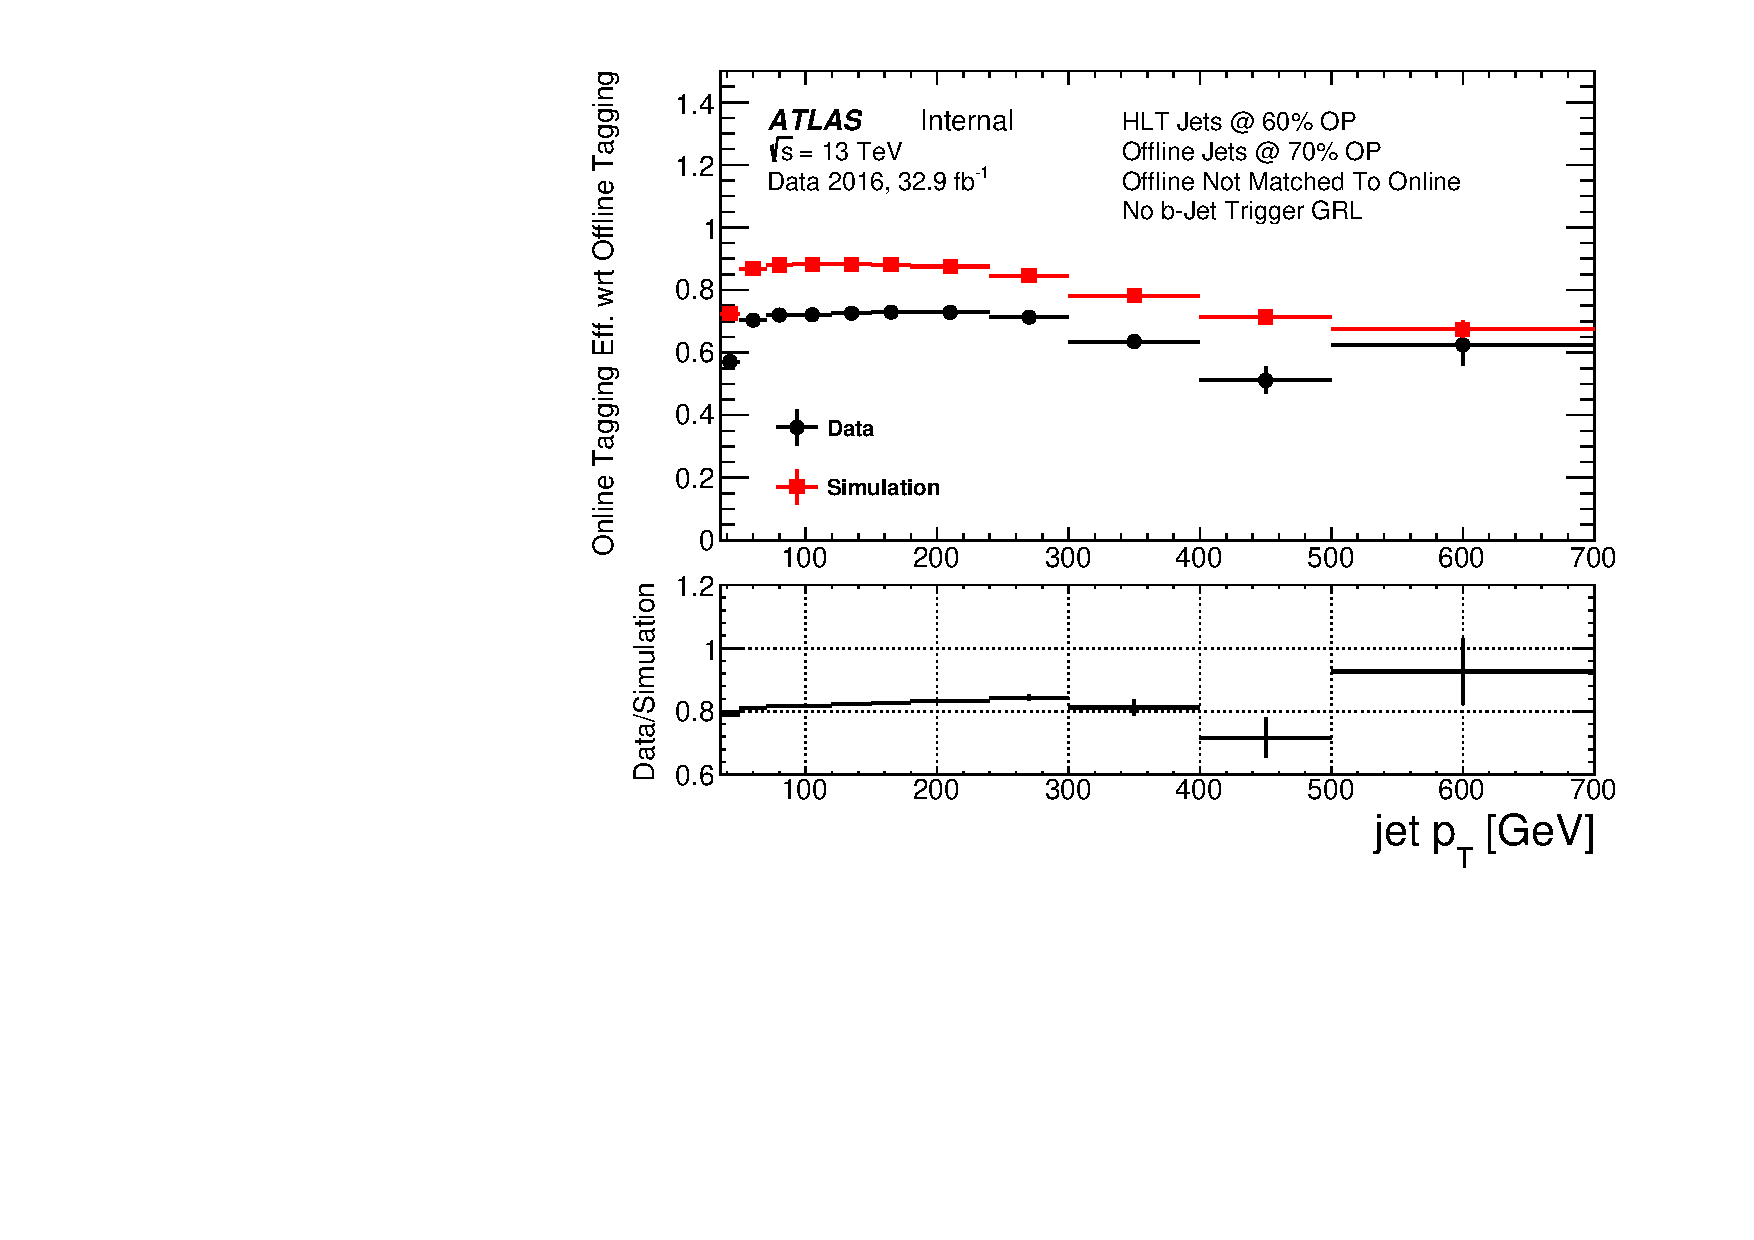
\includegraphics[width=0.47\linewidth, angle=0]{figs/trigger/Full_noGRL_eff_noHLTMatch_jetPt.pdf} }
    \subcaptionbox{Jet-$\eta$}{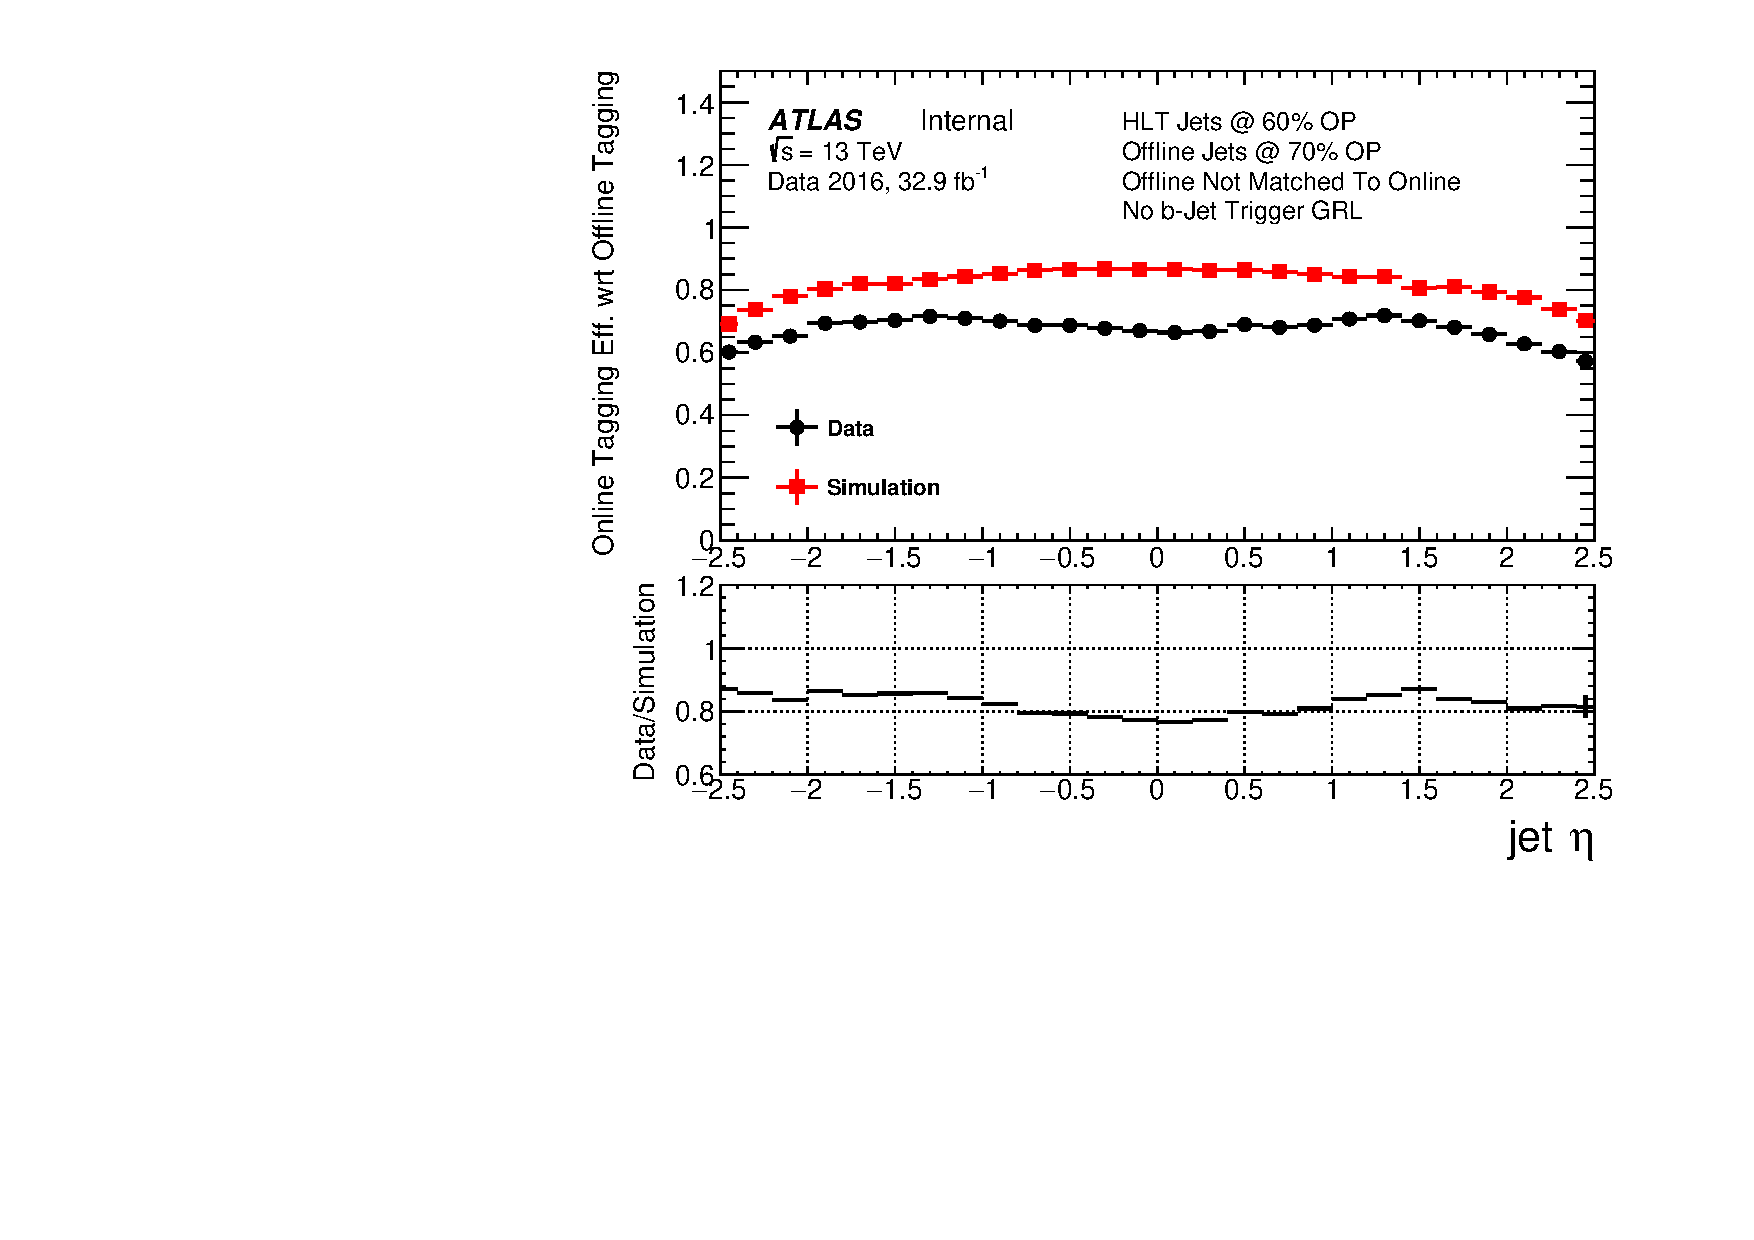
\includegraphics[width=0.47\linewidth, angle=0]{figs/trigger/Full_noGRL_eff_noHLTMatch_jetEta.pdf}}
  \end{center}
  \vspace{-1em}
  \caption[The $b$-jet trigger efficiency in data and simulation
    when the $b$-jet trigger aware GRL is not applied and trigger matching is not required.]
  {The 60\% operating point $b$-jet trigger efficiency with respect to the offline 70\% operating point
    for data (black) and simulation (red) against (a)~jet-\pT{} and (b)~jet-$\eta$.
    The $b$-jet trigger aware GRL is not applied and trigger matching is not required.}
  \label{fig:trig-Full_noGRL_eff_noHLTMatch}
\end{figure}


In Figure~\ref{fig:trig-Full_noGRL_eff_noHLTMatch} the efficiency in data is substantially lower
than the efficiency expected from  simulation and has a different distribution with respect to jet-$\eta$.
The substantial differences need to be investigated and understood. 
The drop in efficiency in the lowest $\pT$ bin (35--50~GeV) is because not all offline jets with a $p_T < 50$~GeV  will have an 
equivalent online jet with $\pT{} > 35$~GeV required to be considered by the $b$-performance trigger. This bias is removed when offline--online matching is required.


%\subsection{Investigation}
%\label{sec:trig-inv}
\newpage

A number of cross-checks were performed to investigate the discrepancy between data and simulation shown in Figure~\ref{fig:trig-Full_noGRL_eff_noHLTMatch}:
including checking for a dependence of the $b$-jet trigger efficiency on the ATLAS detector conditions and the number of pile-up collisions.
It has been discovered that the problem causing the large data-simulation discrepancies was related to hard-scatter primary vertex finding.

As described in Section~\ref{sec:trig-bjet}, in 2016 data the \verb|xPrmVtx| algorithm is used to find the hard-scatter primary vertex (PV) in the $b$-jet trigger.
It has since been uncovered that there was an error in implementation of this algorithm that relates to the online beam-spot position.
The beam-spot position is defined as the centre of the region where the two proton bunches cross in the ATLAS detector.
The beam-spot position is estimated at the trigger-level using the average position of reconstructed primary vertices over many events,
this is known as the online beam-spot position~\cite{trig-onlinePV}.
Online tracks use positions with respect to the online beam-spot position
whilst the \verb|xPrmVtx| algorithm assumes track positions with respect to the origin.
As a result, if the online beamspot $z$-position is far from from the origin then
a \verb|xPrmVtx| PV is often not found and a dummy PV with position at the origin is used by the $b$-jet trigger.
The evidence for this hypothesis is discussed in the remainder of this section.
For brevity, online beamspot $z$-position is henceforth referred to as $z_{\,\text{bs}}^{\text{\,online}}$.  

The exact configuration of the $b$-jet trigger has changed over time to respond to performance issues as they are observed.
The 2016 data-set is therefore split into 3 different \textit{`epochs'} of data, which are defined by the effect on $b$-jet trigger performance of not finding a \verb|xPrmVtx| PV.
The epochs are summarised in Table~\ref{tab:trig-epochs}.
%The relevant conditions of the $b$-jet trigger can be split into three regions of data-taking, which I will refer to as \textit{`epochs'}.
Therefore the $b$-jet trigger efficiency is investigated in each epoch independently.

\begin{table}[!htb]
   \vspace{-0.5em}
  \begin{center}
  \begin{tabular}{ | c || c | c |}
    \hline			
    \textbf{Epoch}  & \textbf{Integrated Luminosity}    & \textbf{Effect if no \textit{xPrmVtx} PV is found} \\ \hline
    \parbox[c]{0.2cm}{\vspace{0.5em}1}      &  \parbox[c]{1cm}{\vspace{0.5em}~0.8~\ifb{}}     & \parbox[t]{4.5cm} {An invalid primary vertex \\is used in online $b$-tagging. \vspace{0.2em}} \\
    \hline                                                     
    \parbox[c]{0.2cm}{\vspace{0.5em}2}      &  \parbox[c]{1.2cm}{\vspace{0.5em}15.2~\ifb{}}     & \parbox[t]{4.5cm}{The $b$-jet trigger will not \\pass the event. \vspace{0.2em} }\\
    \hline                                                
    \parbox[c]{0.2cm}{\vspace{0.5em}3}      &  \parbox[c]{1cm}{\vspace{0.5em}~8.3~\ifb{}}     & \parbox[t]{4.5cm} {A back-up primary vertex \\ finding algorithm is used.\vspace{0.2em}} \\
    \hline
  \end{tabular}
  \end{center}
  %\vspace{pt}
  \vspace{-0.5em}
  \caption{A table summarising the effect of not finding a \textit{xPrmVtx} primary vertex (PV) in each of the epochs of data.}
  \label{tab:trig-epochs}
  \vspace{-0.5em}
\end{table}

\newpage

Firstly let us consider Epoch~1;
Figure~\ref{fig:Epoch1_eff}(a) shows that the $b$-jet trigger efficiency measured in data is ~80-90\% of the efficiency in simulation.
Figure~\ref{fig:Epoch1_eff}(b) shows that the $b$-jet trigger efficiency in Epoch~1 has a strong dependence on $z_{\,\text{bs}}^{\text{\,online}}$;
when $z_{\,\text{bs}}^{\text{\,online}}$ is close to zero the $b$-jet trigger efficiency in data and simulation are comparable
\footnote{\ Simulation is produced with $z_{\,\text{bs}}^{\text{\,online}}$ equal to zero.}
but as $|z_{\,\text{bs}}^{\text{\,online}}|$ increases efficiency falls off steeply.

\begin{figure}[!htb]
  \begin{center}
    \captionsetup[subfigure]{aboveskip=0pt,justification=centering}
    \subcaptionbox{Jet-\pT}{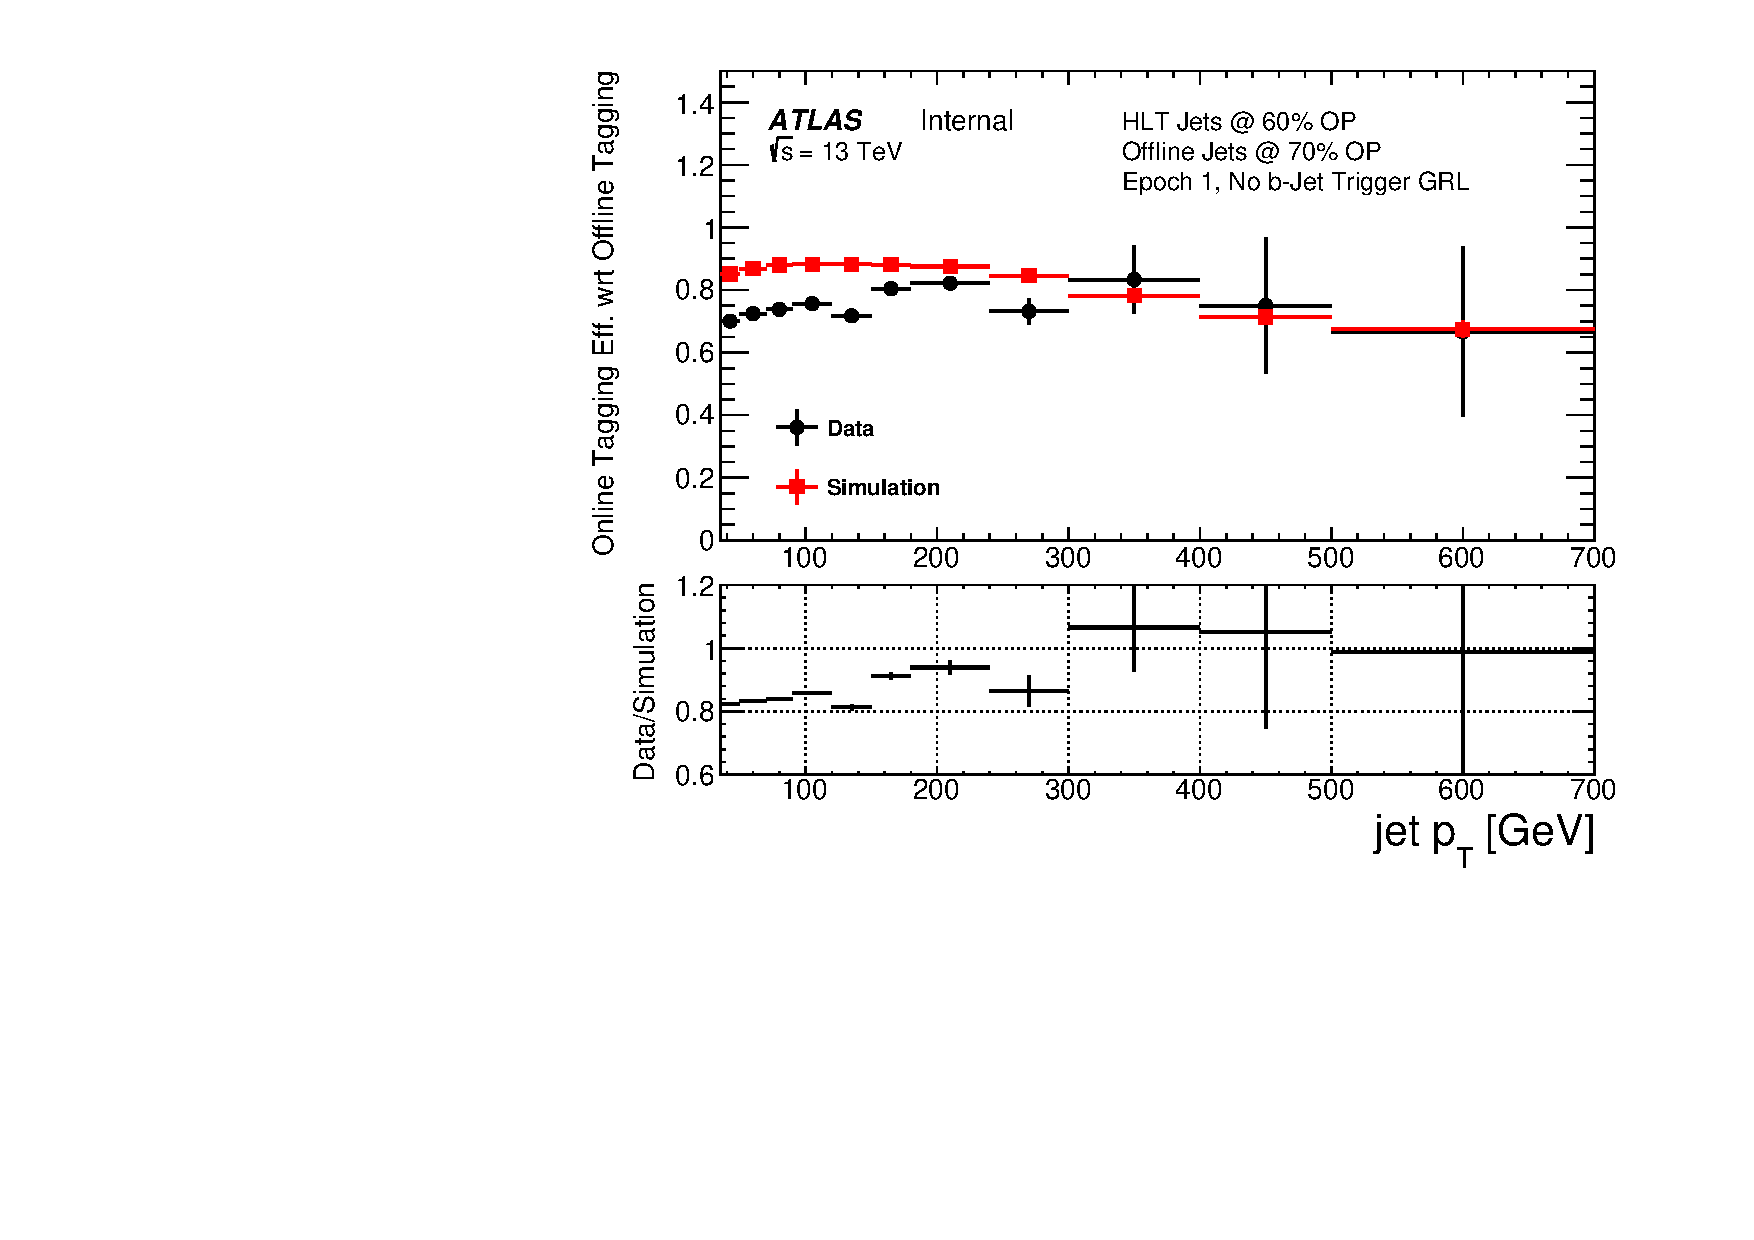
\includegraphics[width=0.45\linewidth, angle=0]{figs/Trigger/Epoch1_noGRL_eff_jetPt.pdf} }
    \subcaptionbox{ $z_{\,\text{bs}}^{\text{\,online}}$}{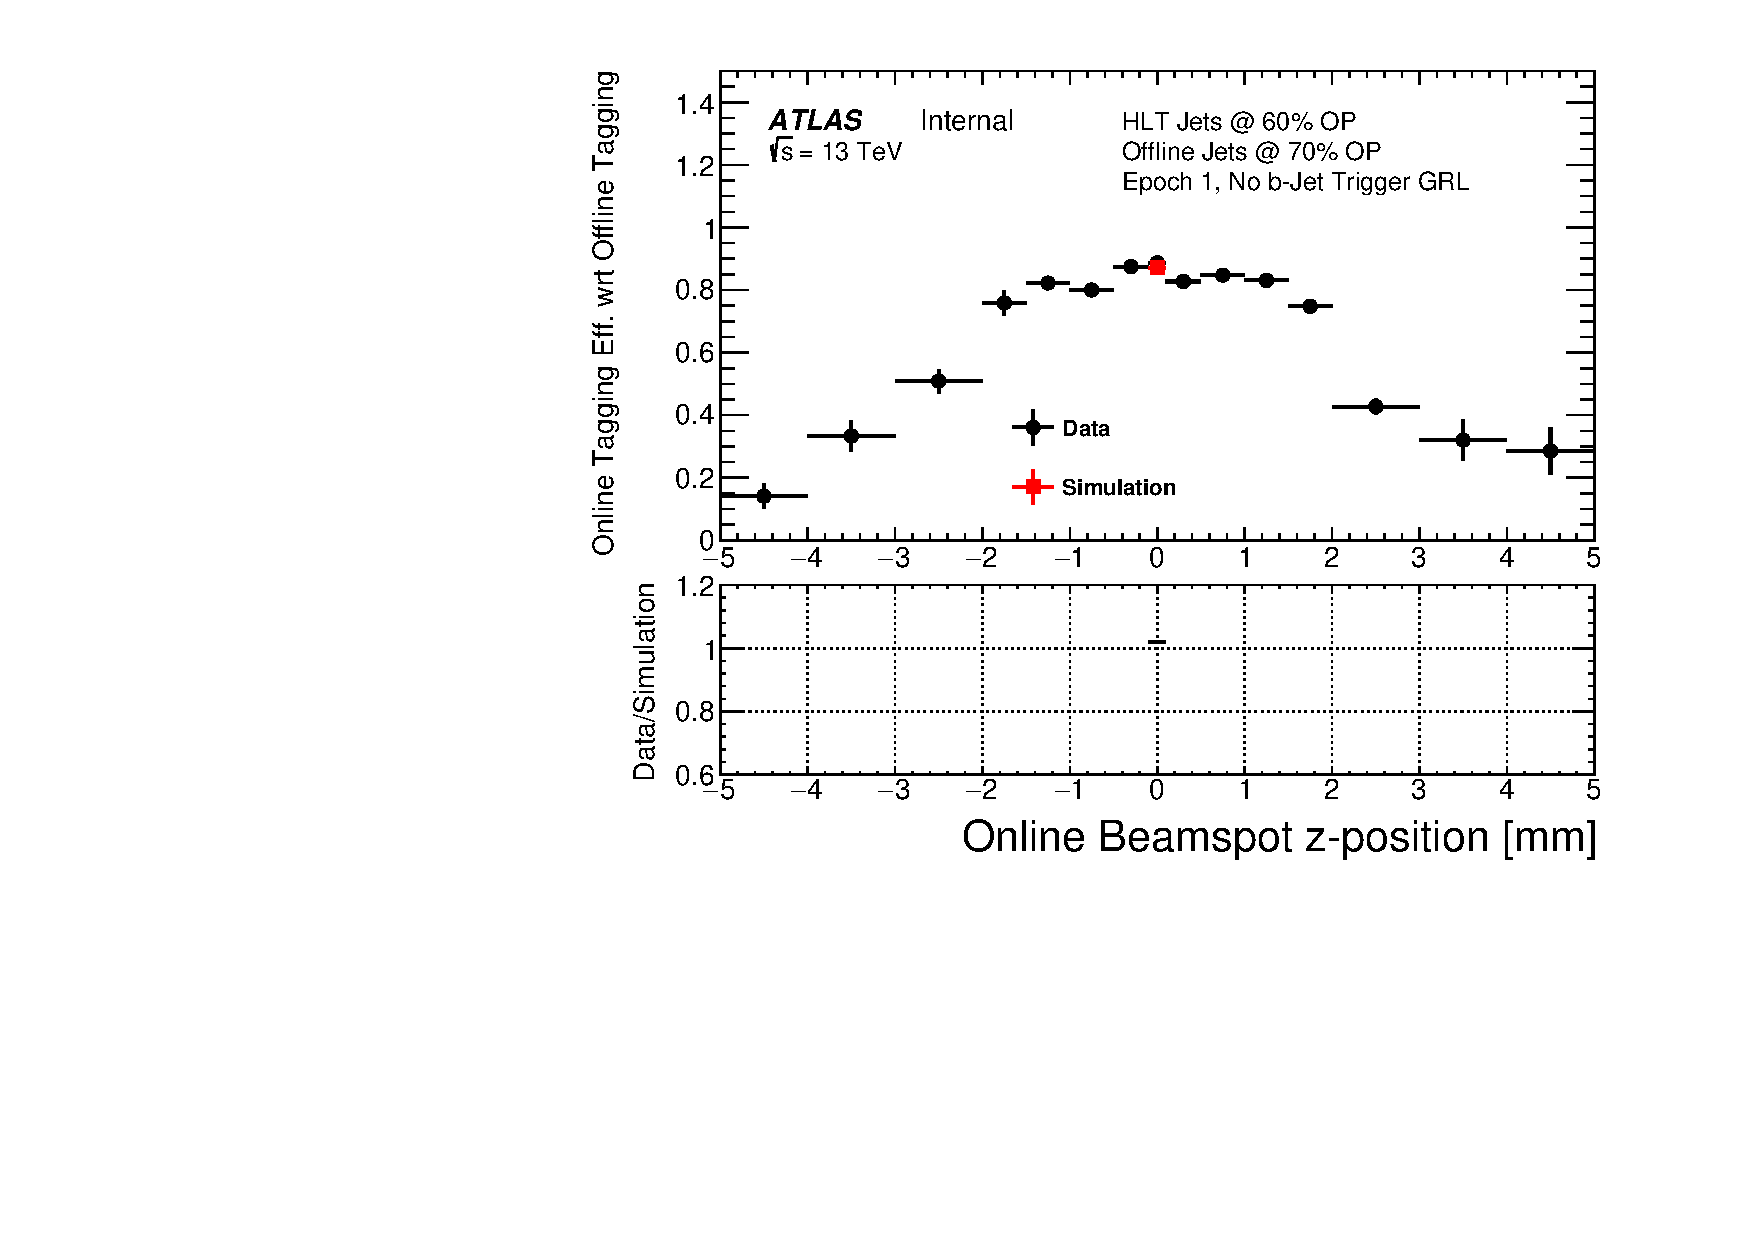
\includegraphics[width=0.45\linewidth, angle=0]{figs/Trigger/Epoch1_noGRL_eff_bs_online_vz.pdf} }
  \end{center}
  \vspace{-1em}
  \caption[The $b$-jet trigger efficiency 
    for data from Epoch~1 and simulation against jet-\pT{} and online beamspot $z$-position.
    The $b$-jet trigger aware GRL has not been applied.]
          {The 60\% operating point $b$-jet trigger efficiency with respect to the offline 70\% operating point
            for data from Epoch~1 (black) and simulation (red) against (a)~jet-\pT{} and online beamspot $z$-position (b).
            The $b$-jet trigger aware GRL has not been applied.}
          \label{fig:Epoch1_eff}
            \vspace{-0.5em}

\end{figure}

To understand this performance the variable \textit{`vertex class'} is studied, which is defined as 0 when a \verb|xPrmVtx| PV is found and 1 if not.
Figure~\ref{fig:Epoch1_vtxClass}(a) shows that when a \verb|xPrmVtx| PV is found the $b$-jet trigger efficiency is reasonably high ($\sim$0.8)
and is comparable between data and simulation (within~5\%),
whilst if no \verb|xPrmVtx| PV is found then efficiency is close to zero in both simulation and data.
However, Figure~\ref{fig:Epoch1_vtxClass}(b) shows that a \verb|xPrmVtx| PV is found in simulation for $>99$\% of the jets,
whilst in data there is $\sim$16\% of events where no \verb|xPrmVtx| PV is found.
Hence, combining the information in Table~\ref{tab:trig-epochs}, Figure~\ref{fig:Epoch1_eff} and Figure~\ref{fig:Epoch1_vtxClass}
it can be concluded that for events in  Epoch~1 where the  $|z_{\,\text{bs}}^{\text{\,online}}|$ is far from zero,
a \verb|xPrmVtx| PV is not found causing a dummy vertex to be used in online $b$-tagging resulting in a low $b$-jet trigger efficiency.
This is the cause of the data/simulation differences observed in Epoch~1. 

\begin{figure}[!ht]
  \begin{center}
    \captionsetup[subfigure]{aboveskip=0pt,justification=centering}
    \subcaptionbox{$\epsilon_{b\text{Trig}}$ against Vertex Class}{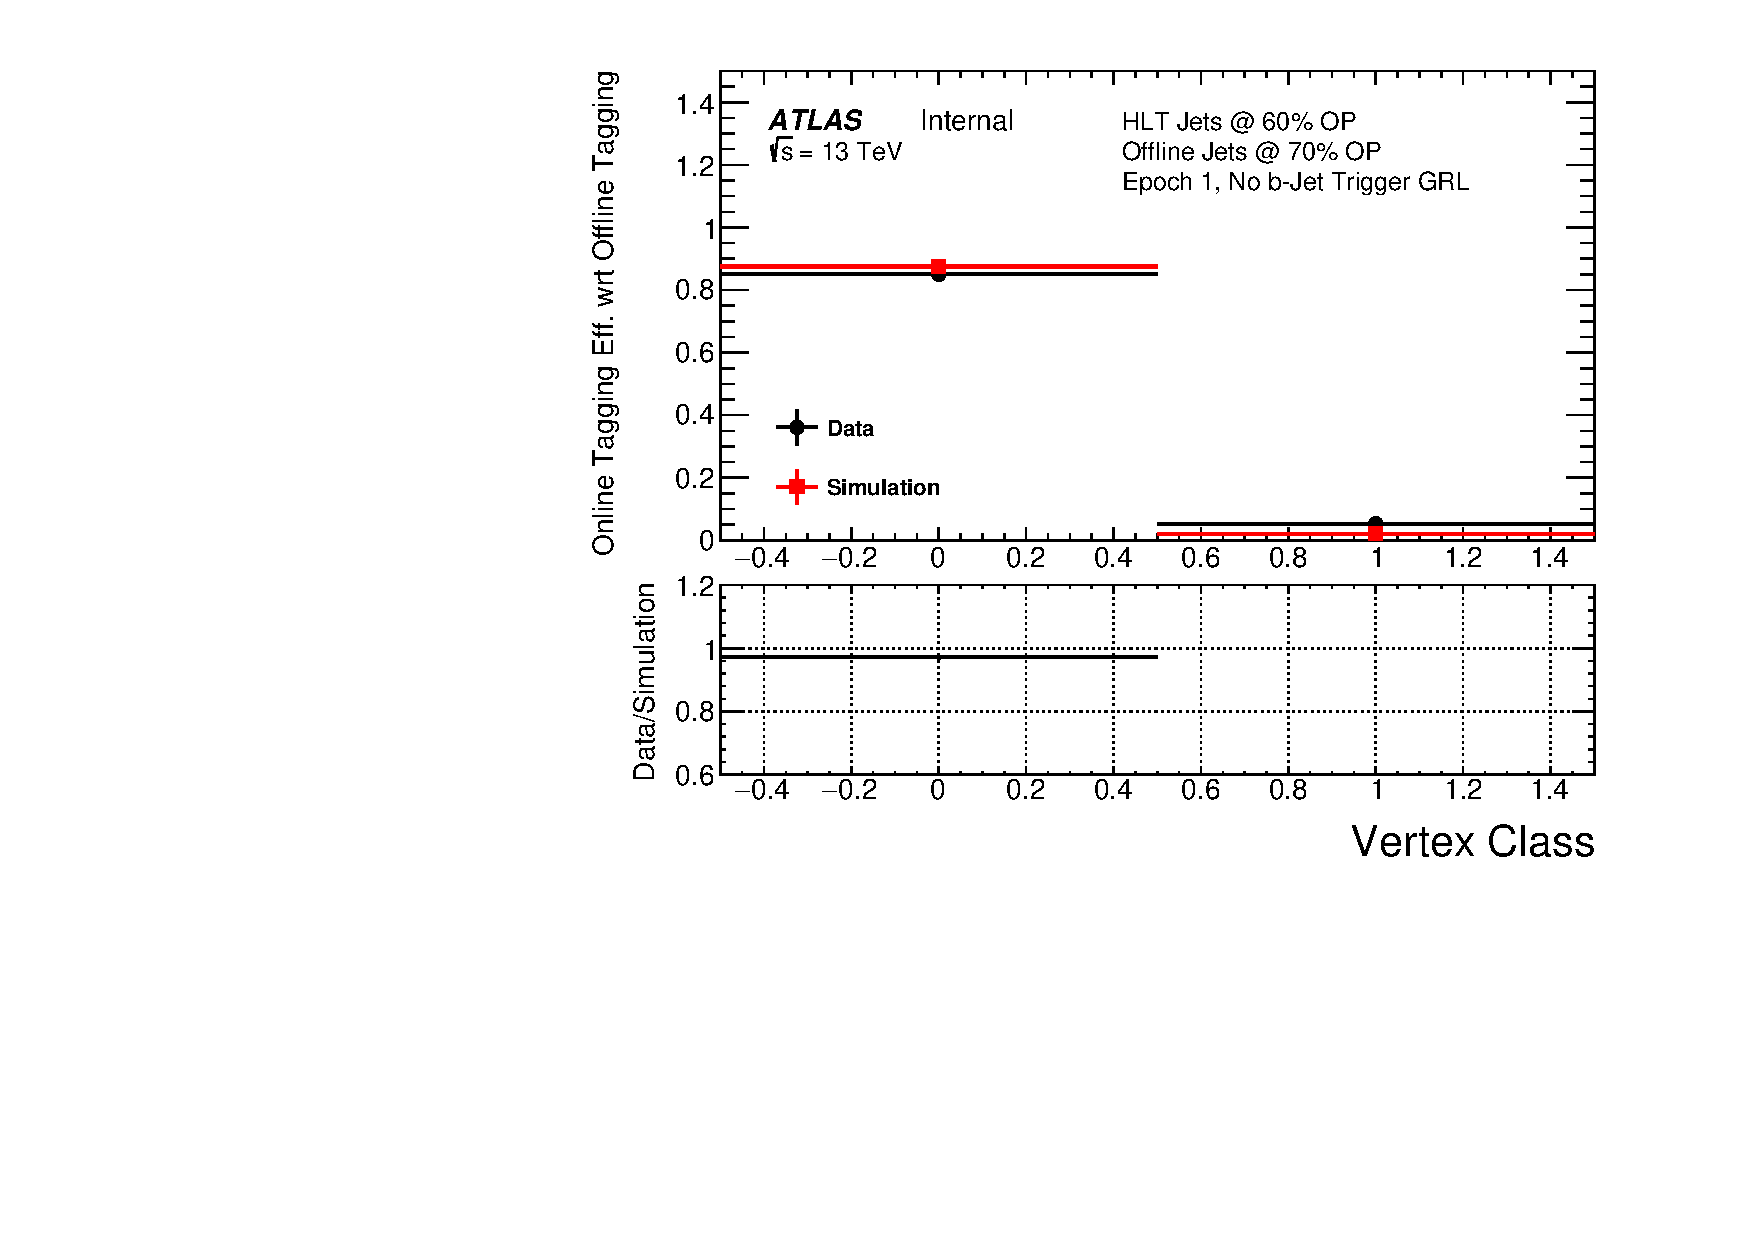
\includegraphics[width=0.45\linewidth, angle=0]{figs/Trigger/Epoch1_noGRL_eff_vtxClass.pdf}}
    \subcaptionbox{Freq. of Offline Jets against Vertex Class}{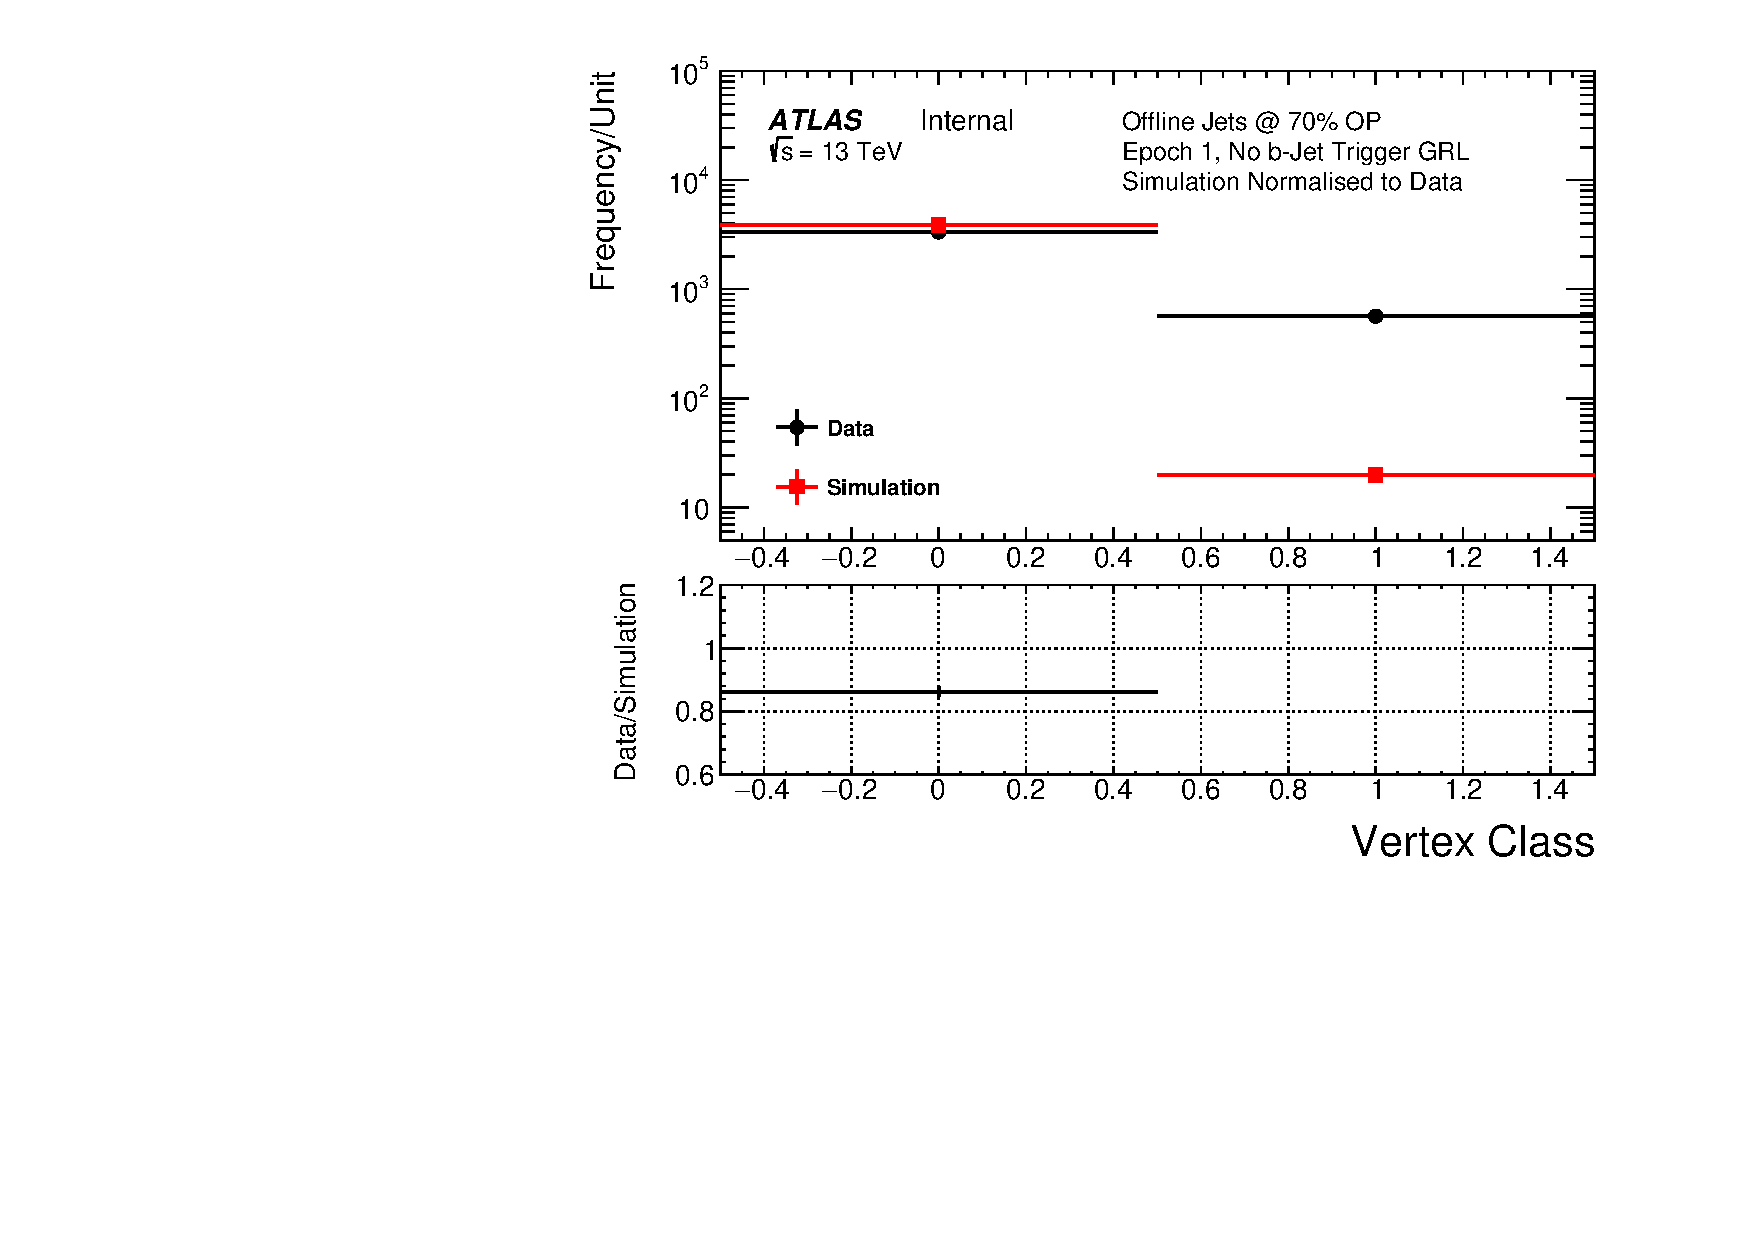
\includegraphics[width=0.45\linewidth, angle=0]{figs/Trigger/Epoch1_noGRL_nOff_vtxClass.pdf}}
  \end{center}
    \vspace{-1em}
  \caption[The $b$-jet trigger efficiency with respect to an offline $b$-tagging
    and  the number of offline jets against vertex class for data from Epoch~1 and simulation.
    The $b$-jet trigger aware GRL has not been applied.]
          {(a) The 60\% operating point $b$-jet trigger efficiency with respect to the offline 70\% operating point
    and  (b) the number of offline jets $b$-tagged at the 70\% operating point that match a HLT trigger jet
    against vertex class for data from Epoch~1 (black) and simulation (red).
    Vertex class is defined as 0 when a \textit{xPrmVtx} vertex is found and 1 if not.
    The $b$-jet trigger aware GRL has not been applied.}
    \label{fig:Epoch1_vtxClass}
\end{figure}



%\begin{figure}[!ht]
%\begin{center}
%  \includegraphics[width=0.47\linewidth, angle=0]{figs/Trigger/Epoch1_bPerfEff_leadingJet_jetPt.pdf}
%  \includegraphics[width=0.47\linewidth, angle=0]{figs/Trigger/Epoch1_bPerfEff_leadingJet_bs_online_vz.pdf}
%\end{center}
%\caption{online primary vertex efficiency, $\epsilon_{\text{PV}}$, for data from Period A (black) and simulation (red) against jet-pT~(left) and online beamspot $z$-position (right).}
%\label{fig:Epoch1_bperf}
%\end{figure}

%In Epoch~2, there is a similar problem to Epoch~1, but there is a subtle difference which requires us to look at this region in a different way.
%As in Epoch~1, when  $z_{\,\text{bs}}^{\text{\,online}}$ is far from zero then a \verb|xPrmVtx| PV is not found.
In Epoch~2 if a \verb|xPrmVtx| PV is not found, the $b$-jet trigger procedure terminates whilst processing the event and therefore the trigger does not pass the event.
As the $b$-jet trigger procedure terminates, the $b$-performance triggers will also not be passed when no \verb|xPrmVtx| PV is found.
This means that events with no \verb|xPrmVtx| PV are lost in both numerator and denominator when calculating the $b$-jet trigger efficiency.
Therefore the measured $b$-jet trigger efficiency using the $b$-performance triggers is consistent in data and simulation;
Figure~\ref{fig:Epoch2_eff} shows the $b$-jet trigger efficiency measured in data to be in agreement with simulation within 5\%.
This is the reason it was necessary to relax the offline--online jet matching to accurately represent the full data-simulation discrepancy in Figure~\ref{fig:trig-Full_noGRL_eff_noHLTMatch}.

\begin{figure}[!htb]
\begin{center}
  \captionsetup[subfigure]{aboveskip=0pt,justification=centering}
  \subcaptionbox{Jet-\pT}{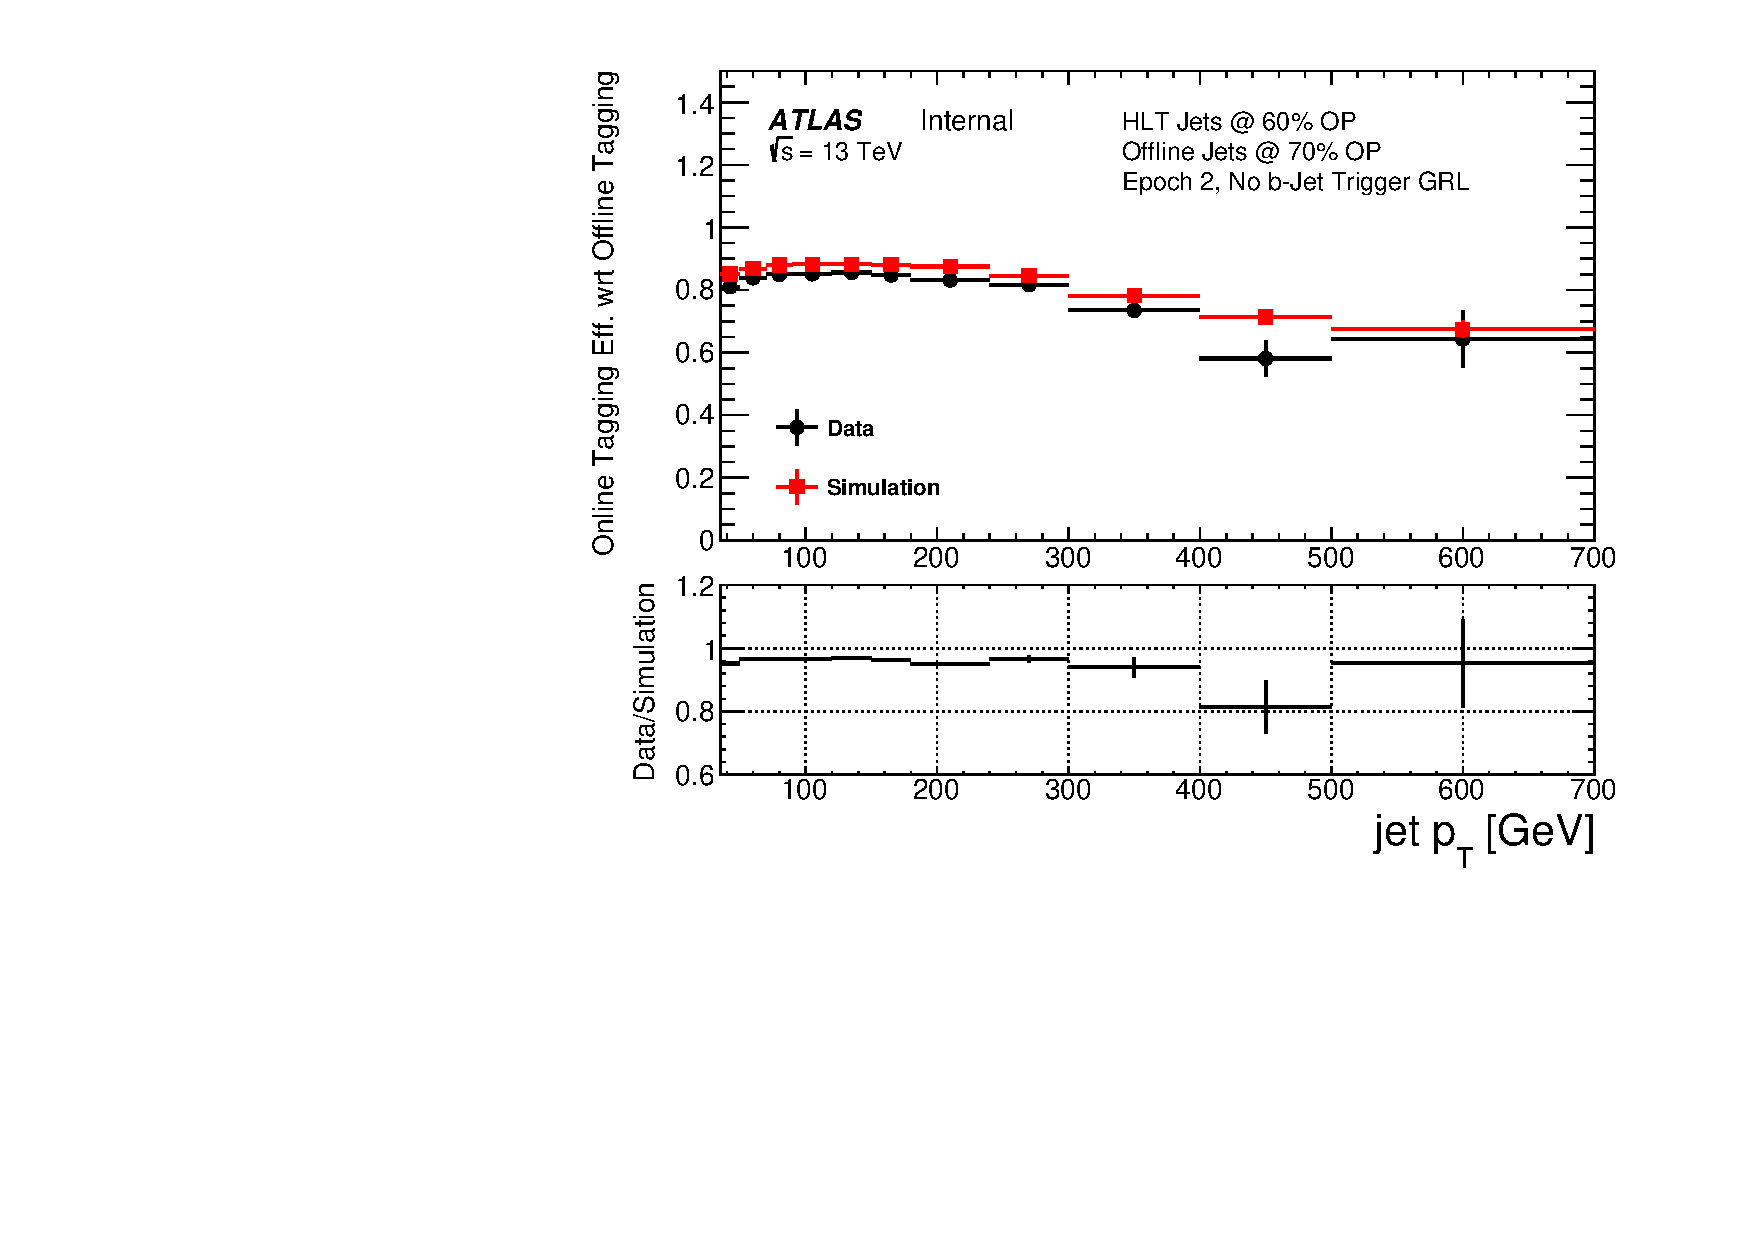
\includegraphics[width=0.47\linewidth, angle=0]{figs/Trigger/Epoch2_noGRL_eff_jetPt.pdf}}     
  \subcaptionbox{$z_{\,\text{bs}}^{\text{\,online}}$}{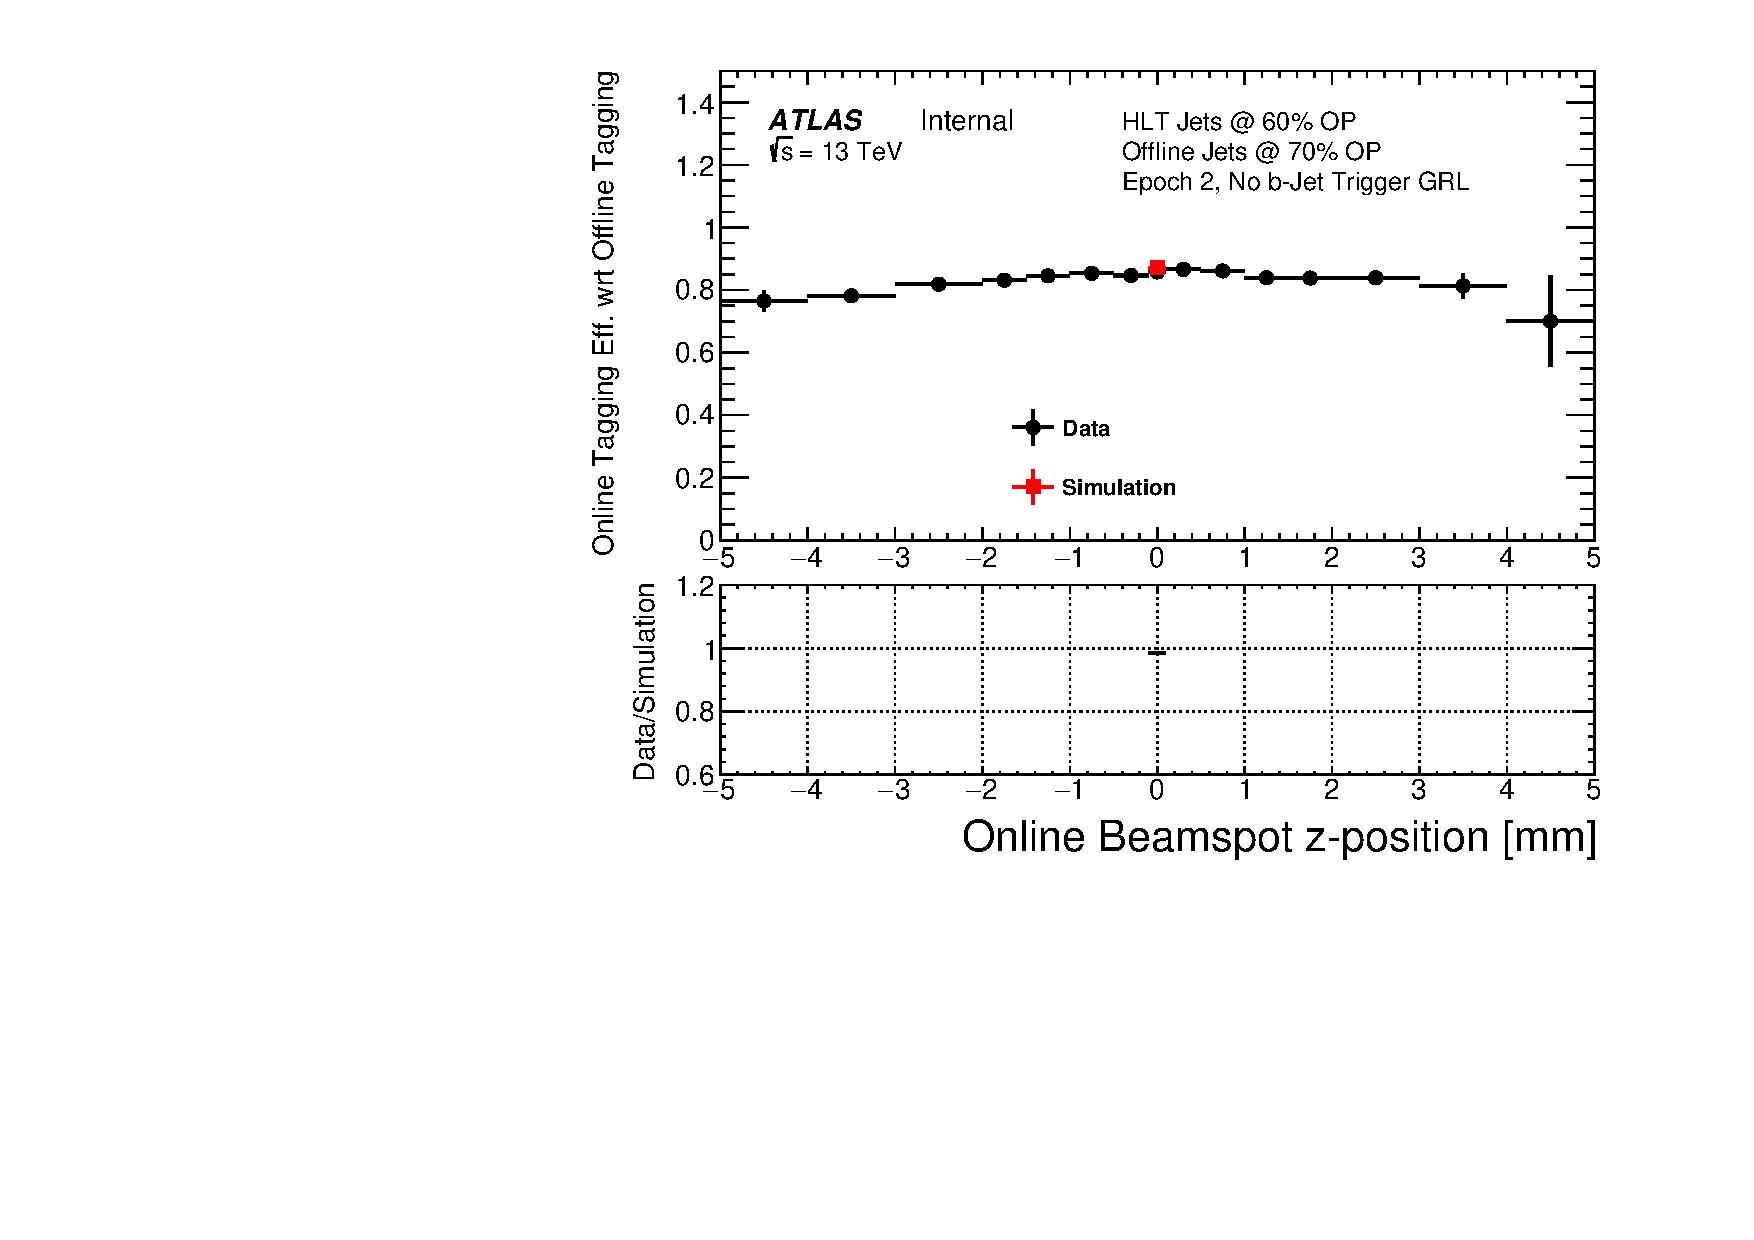
\includegraphics[width=0.47\linewidth, angle=0]{figs/Trigger/Epoch2_noGRL_eff_bs_online_vz.pdf}}
  %\subcaptionbox{??}{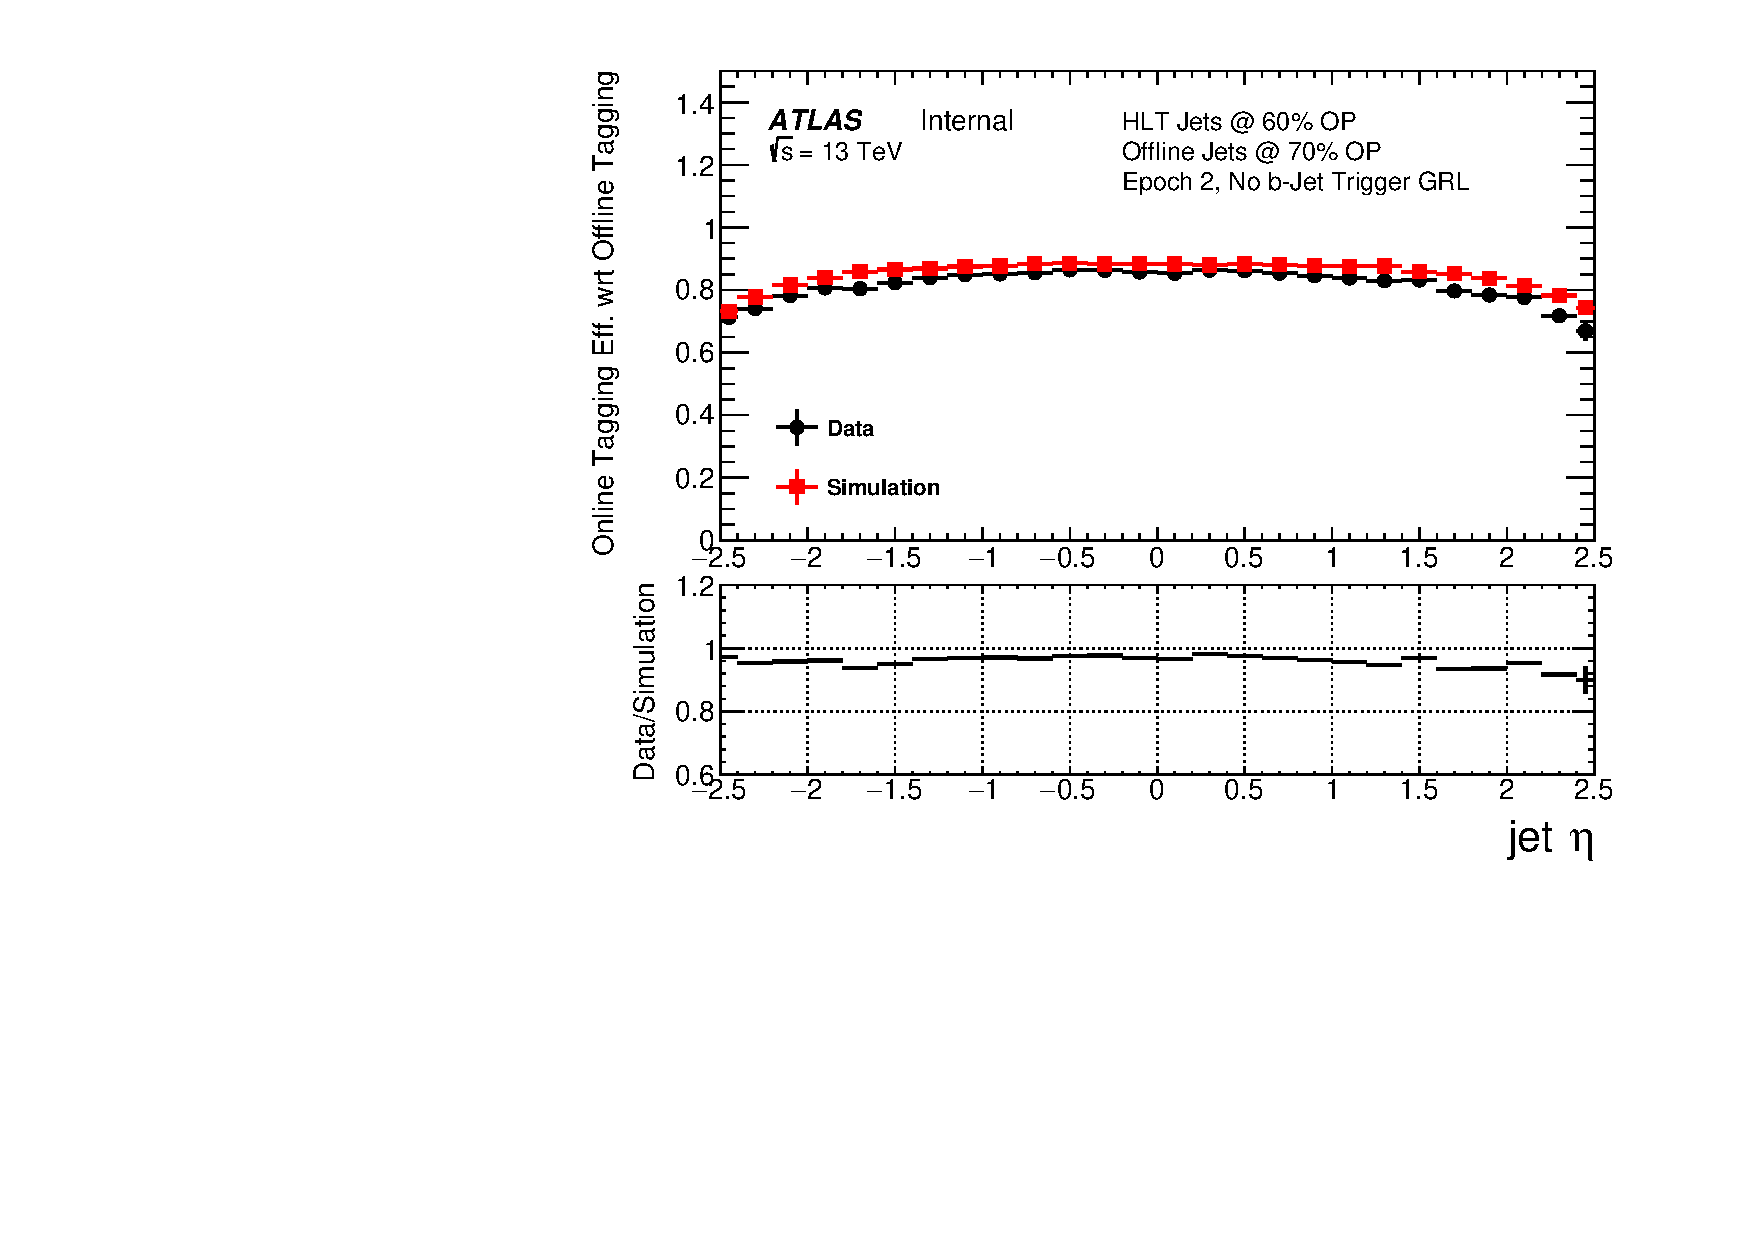
\includegraphics[width=0.47\linewidth, angle=0]{figs/Trigger/Epoch2_noGRL_eff_jetEta.pdf}} \\
  %\subcaptionbox{??}{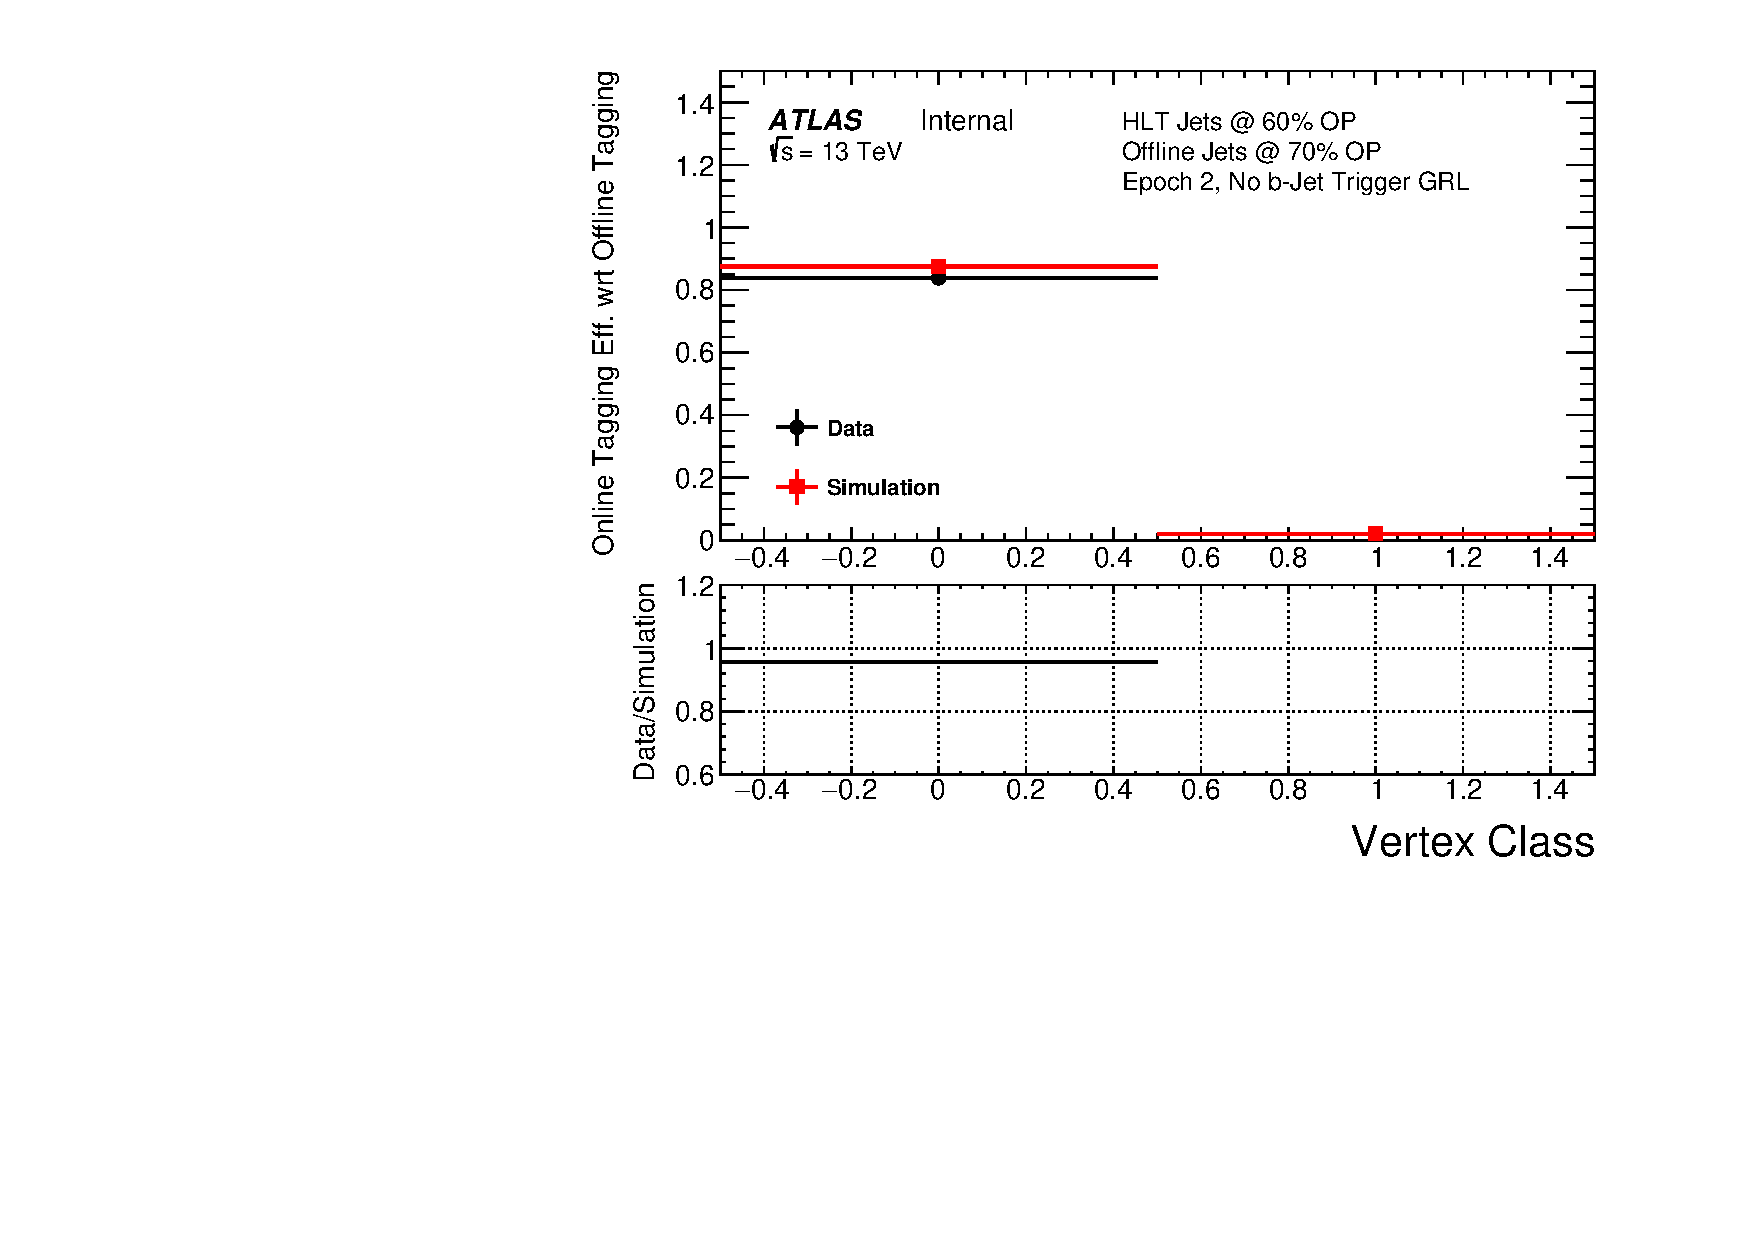
\includegraphics[width=0.47\linewidth, angle=0]{figs/Trigger/Epoch2_noGRL_eff_vtxClass.pdf}}
\end{center}
\vspace{-1em}
\caption[
  The $b$-jet trigger efficiency 
  for data from Epoch~2 and simulation against jet-\pT{} and online beamspot $z$-position.
  The $b$-jet trigger aware GRL has not been applied.]
        {
  The 60\% operating point $b$-jet trigger efficiency with respect to the offline 70\% operating point
  for data from Epoch~2 (black) and simulation (red) against (a) jet-\pT{} and (b) online beamspot $z$-position.
  The $b$-jet trigger aware GRL has not been applied.}
\label{fig:Epoch2_eff}
\end{figure}

Therefore, in Epoch~2 it is necessary to account for the cases when a \verb|xPrmVtx| PV is not found
by measuring the online primary vertex efficiency, $\epsilon_{\text{PV}}$,
which is the efficiency that there is a primary vertex in the event.
$\epsilon_{\text{PV}}$ is calculated in Epoch~2 by dividing the number of events that pass the single muon $b$-performance trigger
by the number of events that pass the equivalent single muon trigger with no $b$-performance functionality
\footnote{ Specifically $\epsilon_{\text{PV}}$ = Number of events that pass \textit{HLT\_mu26\_imedium\_2j35\_bperf} divided by the number that pass \textit{HLT\_mu26\_imedium}.}.
The denominator of $\epsilon_{\text{PV}}$ has no $b$-jet trigger dependency so is unaffected by the \verb|xPrmVtx| algorithm.
$\epsilon_{\text{PV}}$ is an event level quantity that must be measured with respect to other event level quantities, such as leading jet-\pT.

Figure~\ref{fig:Epoch2_bperf}(a) shows that $\epsilon_{\text{PV}}$ has a data/simulation ratio of around 80\%  which is similar to that shown in Figure~\ref{fig:Epoch1_eff}.
Figure~\ref{fig:Epoch2_bperf}(b) shows that $\epsilon_{\text{PV}}$ has a similar shape with respect to  $z_{\,\text{bs}}^{\text{\,online}}$ as observed in Epoch~1,
shown in Figure~\ref{fig:trig-Full_noGRL_eff_noHLTMatch}.
Furthermore in Figure~\ref{fig:Epoch2_bperf}(c) it is shown that there is a reduced online primary vertex efficiency at smaller values of absolute leading jet-$\eta$.
This shows that the inefficiency in finding a \verb|xPrmVtx| PV causes a kinematic bias with respect to leading jet-$\eta$. %,
%an effect that must be accounted for in the final efficiency measurement.

\begin{figure}[!ht]
\begin{center}
  \captionsetup[subfigure]{aboveskip=0pt,justification=centering}
  \subcaptionbox{Leading jet-\pT}{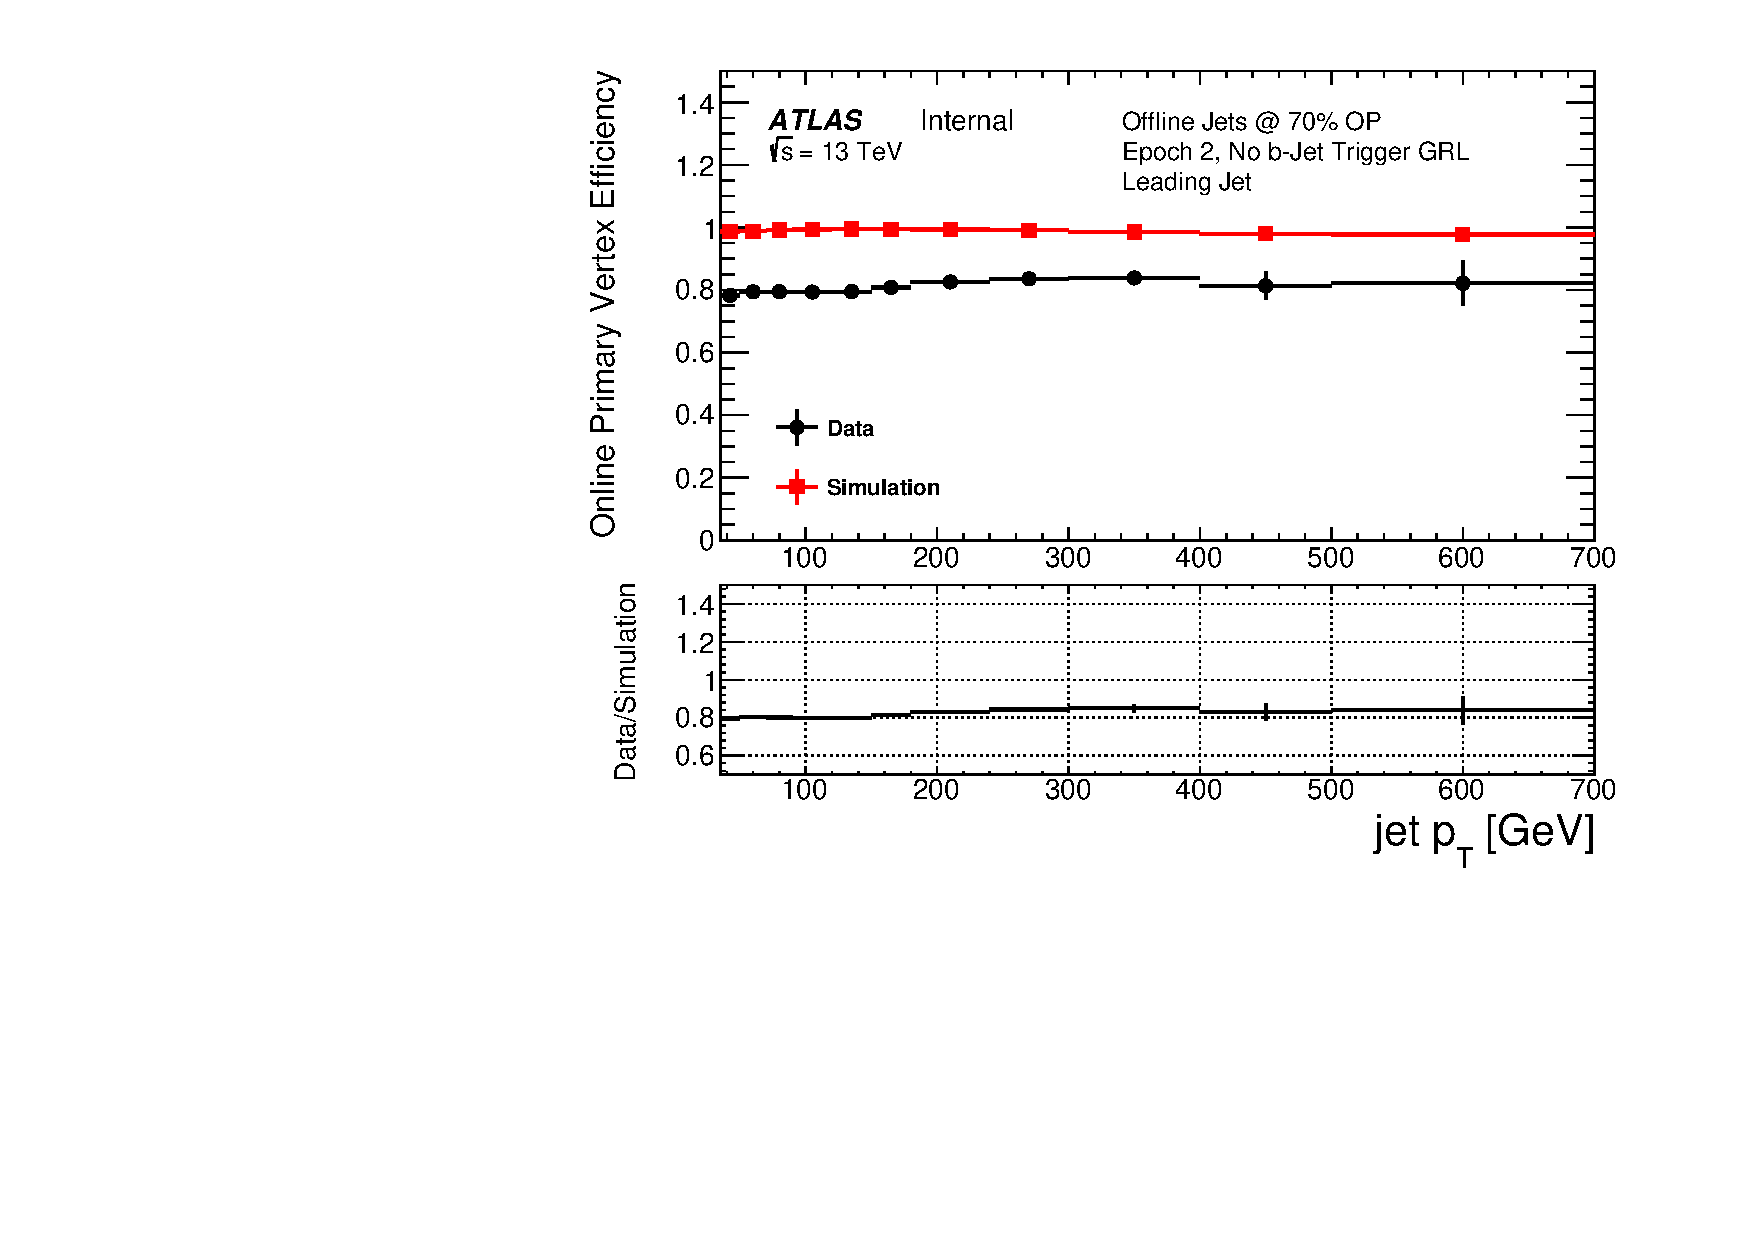
\includegraphics[width=0.47\linewidth, angle=0]{figs/Trigger/Epoch2_noGRL_bPerfEff_leadingJet_jetPt.pdf}}
  \subcaptionbox{$z_{\,\text{bs}}^{\text{\,online}}$}{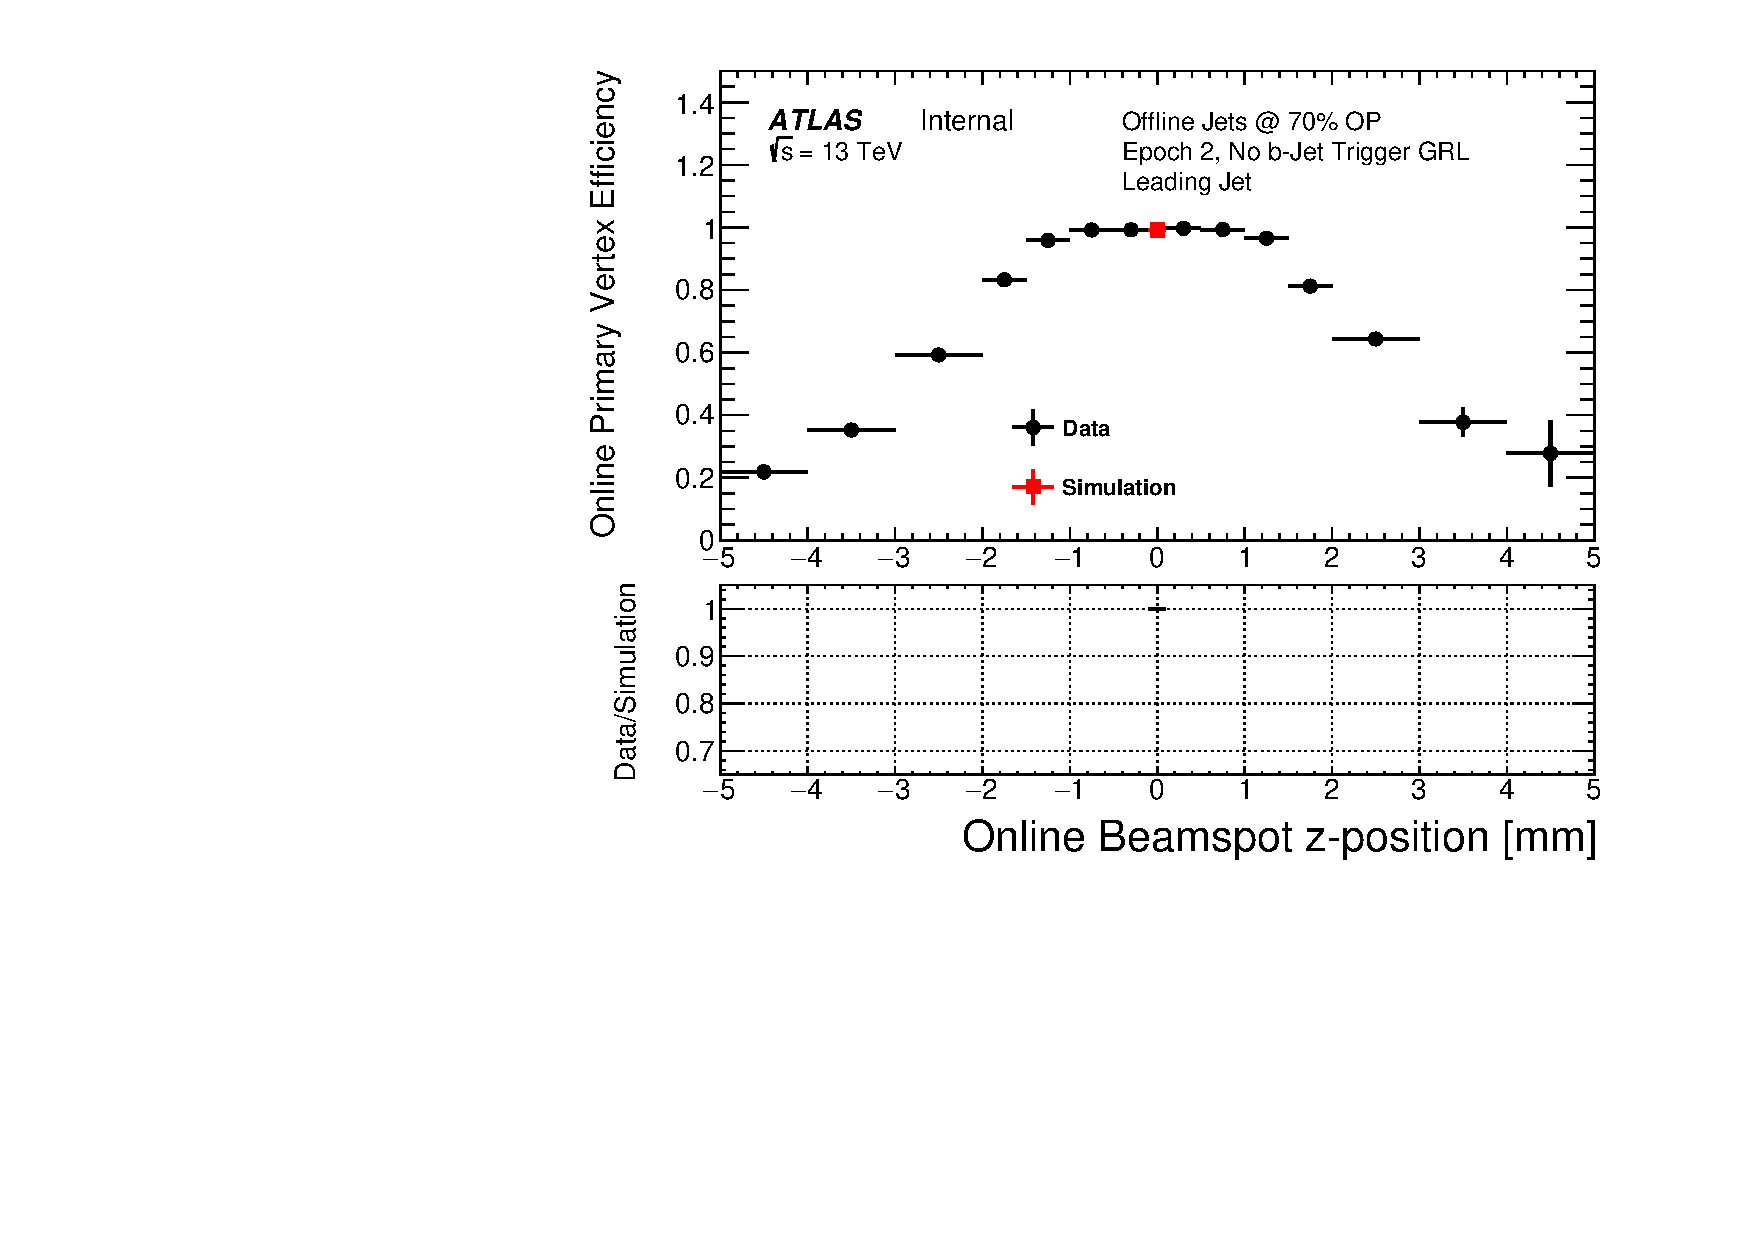
\includegraphics[width=0.47\linewidth, angle=0]{figs/Trigger/Epoch2_noGRL_bPerfEff_leadingJet_bs_online_vz.pdf}}\\
  \subcaptionbox{Leading jet-$\eta$}{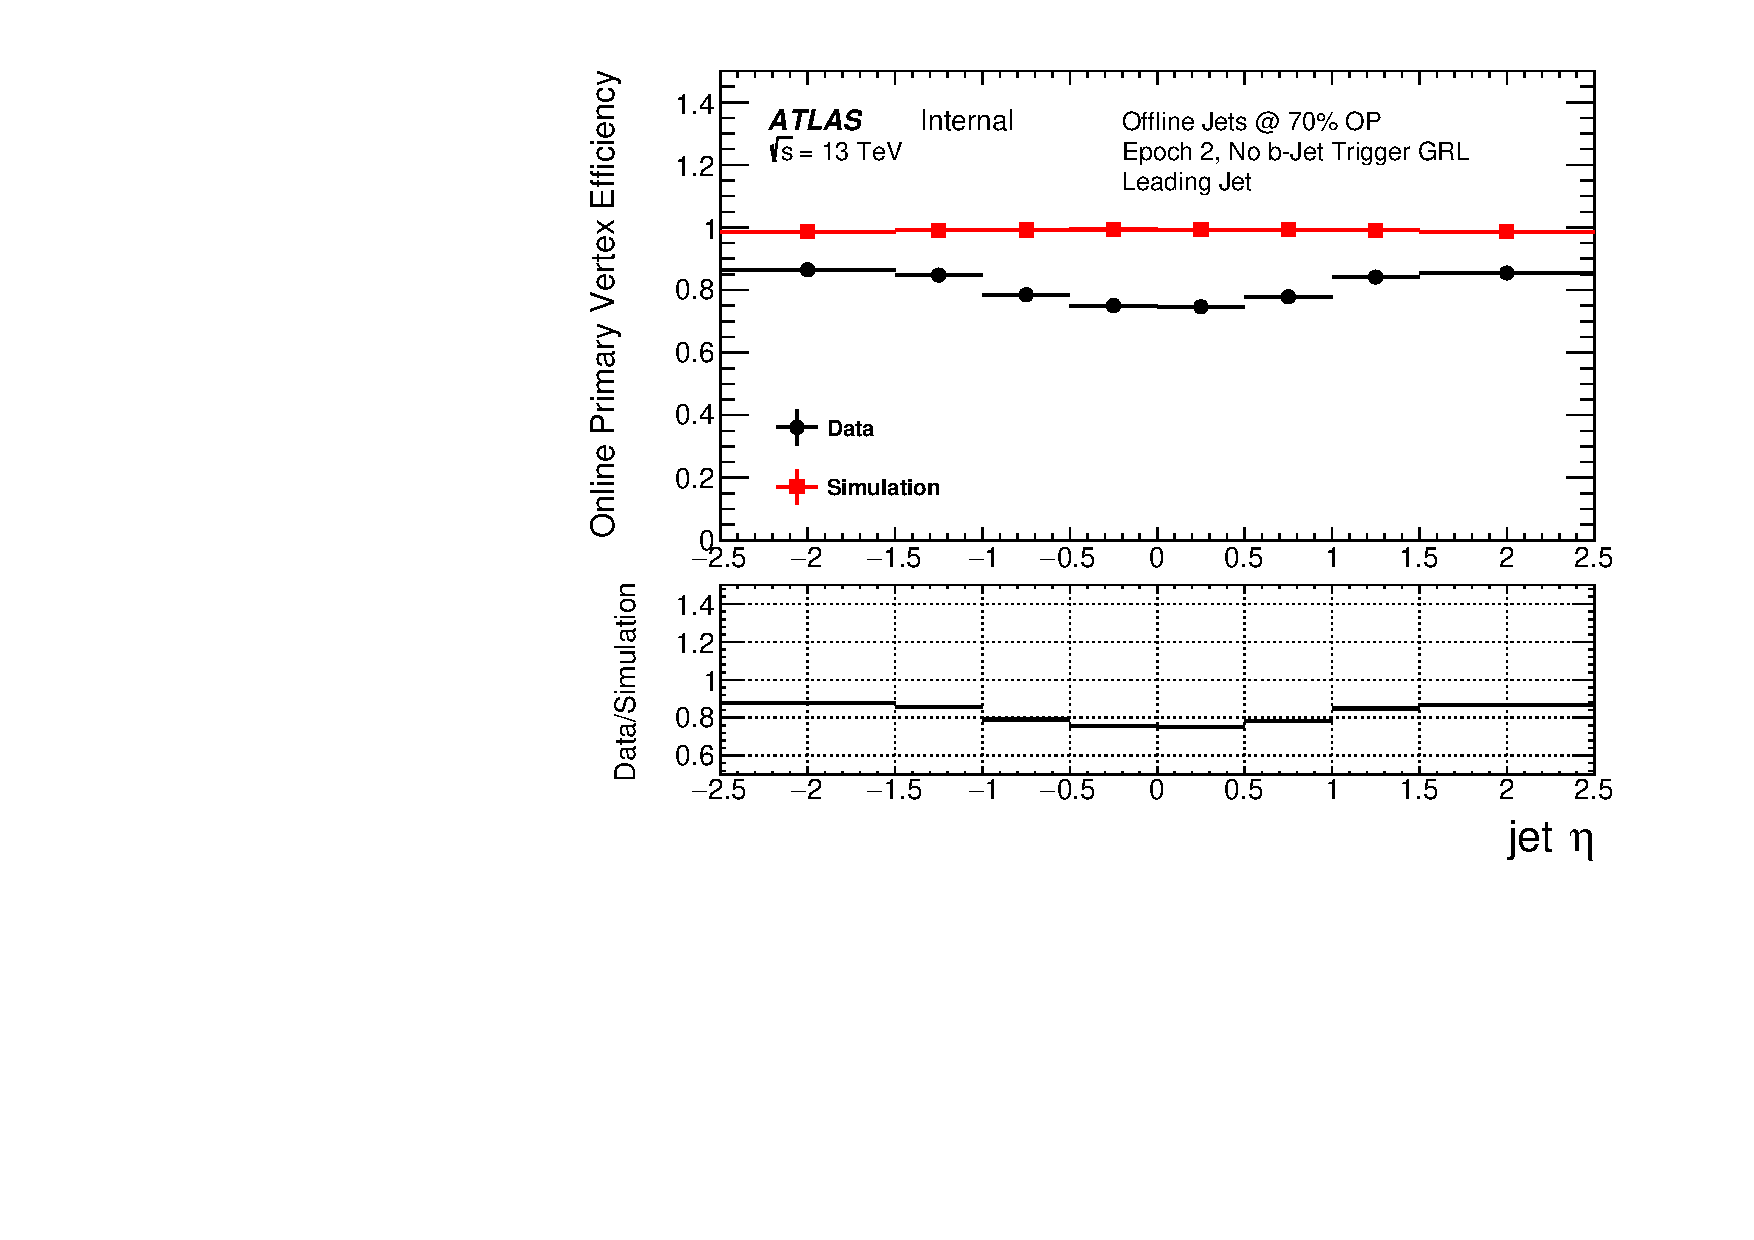
\includegraphics[width=0.47\linewidth, angle=0]{figs/Trigger/Epoch2_noGRL_bPerfEff_leadingJet_jetEta.pdf}}
\end{center}
\vspace{-1em}
\caption[The online primary vertex efficiency for data from Epoch~2 and simulation against leading-jet \pT{}, online beamspot $z$-position
  and leading jet-\eta. The $b$-jet trigger aware GRL has not been applied.]
        {The online primary vertex efficiency, $\epsilon_{\text{PV}}$, for data from Epoch~2 (black) and simulation (red) against (a) leading-jet \pT{}, (b) online beamspot $z$-position
  and (c) leading jet-\eta.
  The $b$-jet trigger aware GRL has not been applied.}
\label{fig:Epoch2_bperf}
\end{figure}


%\begin{figure}[!ht]
%\begin{center}
%  \captionsetup[subfigure]{aboveskip=0pt,justification=centering}
%\end{center}
%\caption{online primary vertex efficiency, $\epsilon_{\text{PV}}$, for data from Epoch~2 (black) and simulation (red) against leading-jet \eta{}.}
%\label{fig:Epoch2_bperf_eta}
%\end{figure}

For Epoch~3, when no \verb|xPrmVtx| PV is found a backup PV finding algorithm is used.
The backup algorithm, known as \verb|EFHist|, is the PV finding algorithm used in 2015 data and finds the PV through a basic histogramming of the tracks.
The simplicity of the \verb|EFHist| algorithm means that a PV is always found.
Figure~\ref{fig:Epoch3_eff} shows the $b$-jet trigger efficiency in Epoch~3 against jet-\pT, jet-$\eta$,  $z_{\,\text{bs}}^{\text{\,online}}$ and vertex class (as defined above).
In Epoch~3 the $b$-jet trigger efficiency measured in data is within 5\% of simulation and there is no shape difference between the two with respect to jet-$\eta$.
In addition, it is shown that in Epoch~3 there is no dependence of the $b$-jet trigger efficiency on $z_{\,\text{bs}}^{\text{\,online}}$ or vertex class.
This demonstrates that the use of a backup finding algorithm alleviates the $b$-jet trigger performance issues observed in Epoch~1 and Epoch~2.

\begin{figure}[!htb]
\begin{center}
  \captionsetup[subfigure]{aboveskip=0pt,justification=centering}
  \subcaptionbox{Jet-\pT}{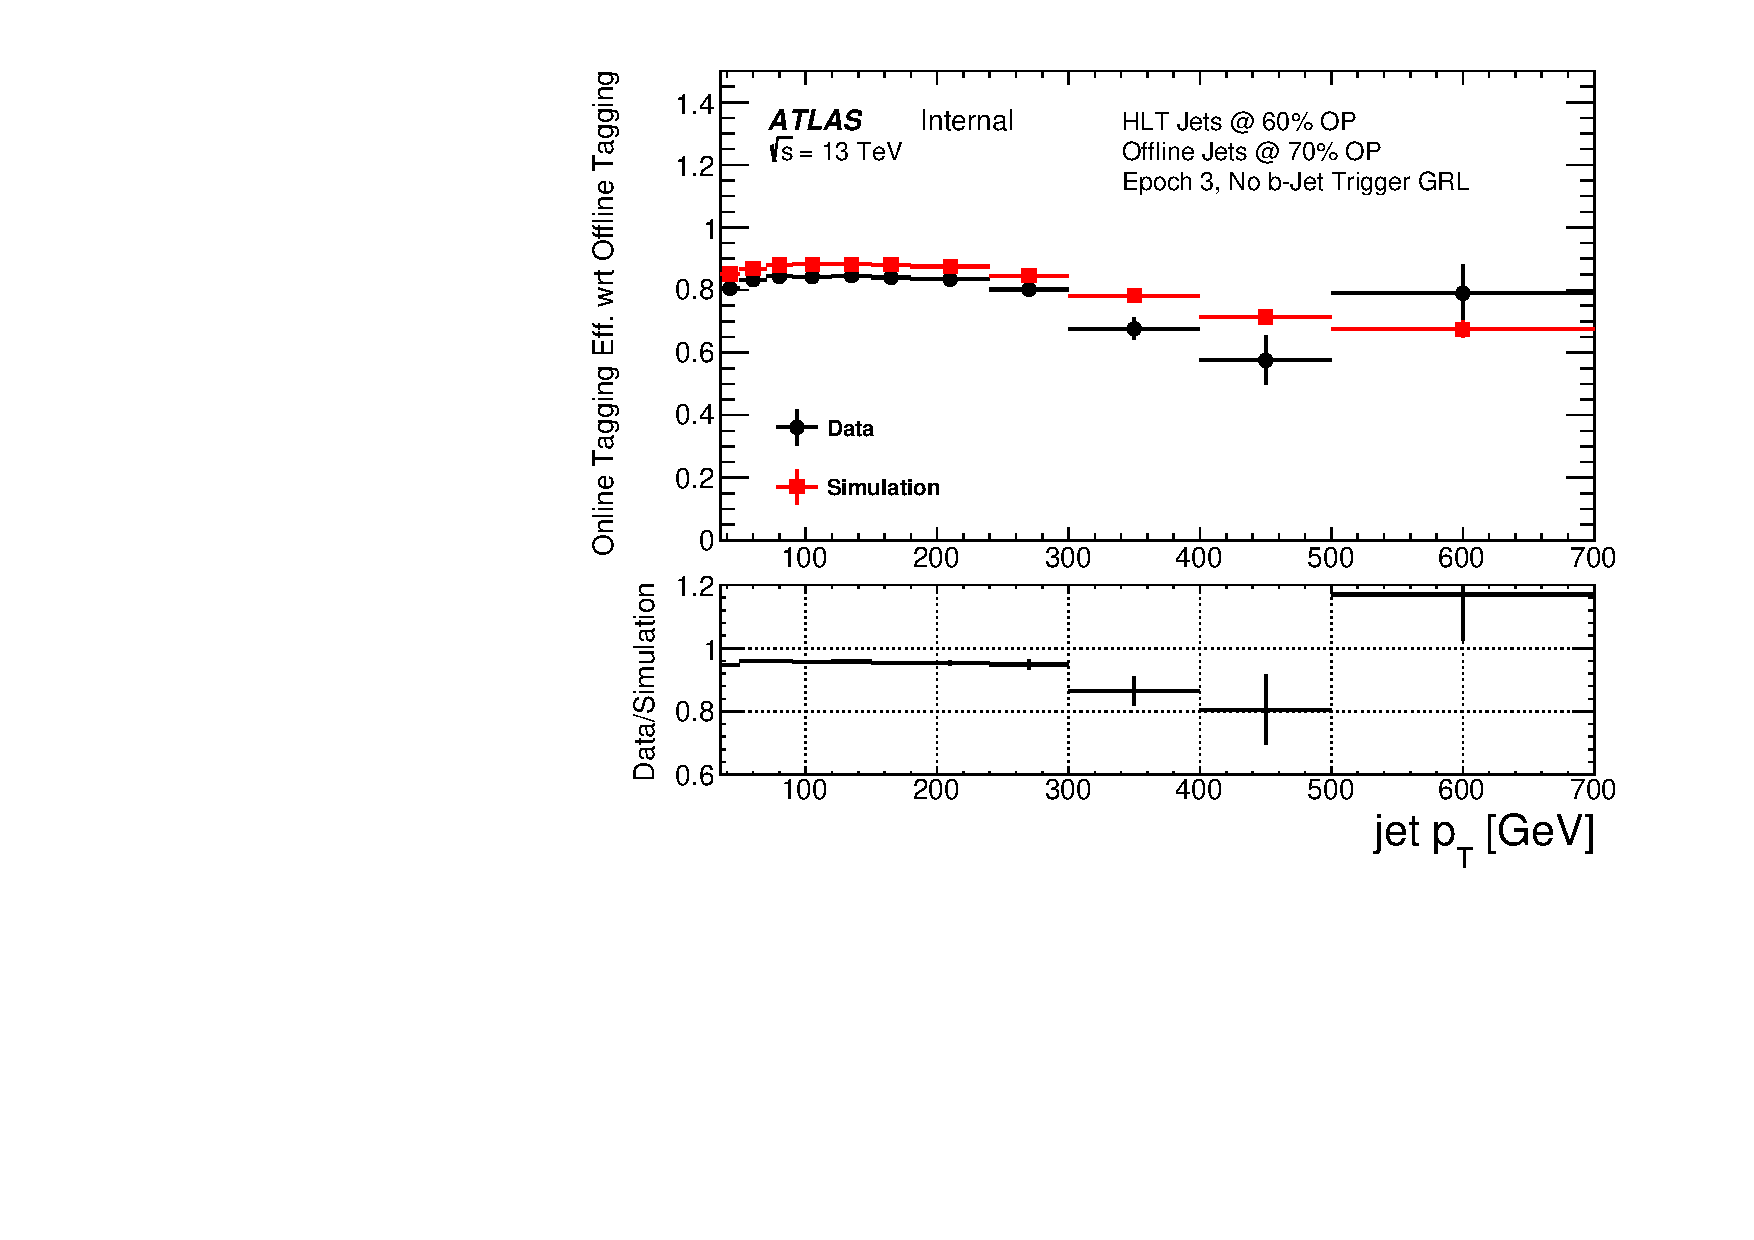
\includegraphics[width=0.47\linewidth, angle=0]{figs/Trigger/Epoch3_noGRL_eff_jetPt.pdf}}
  \subcaptionbox{Jet-$\eta$}{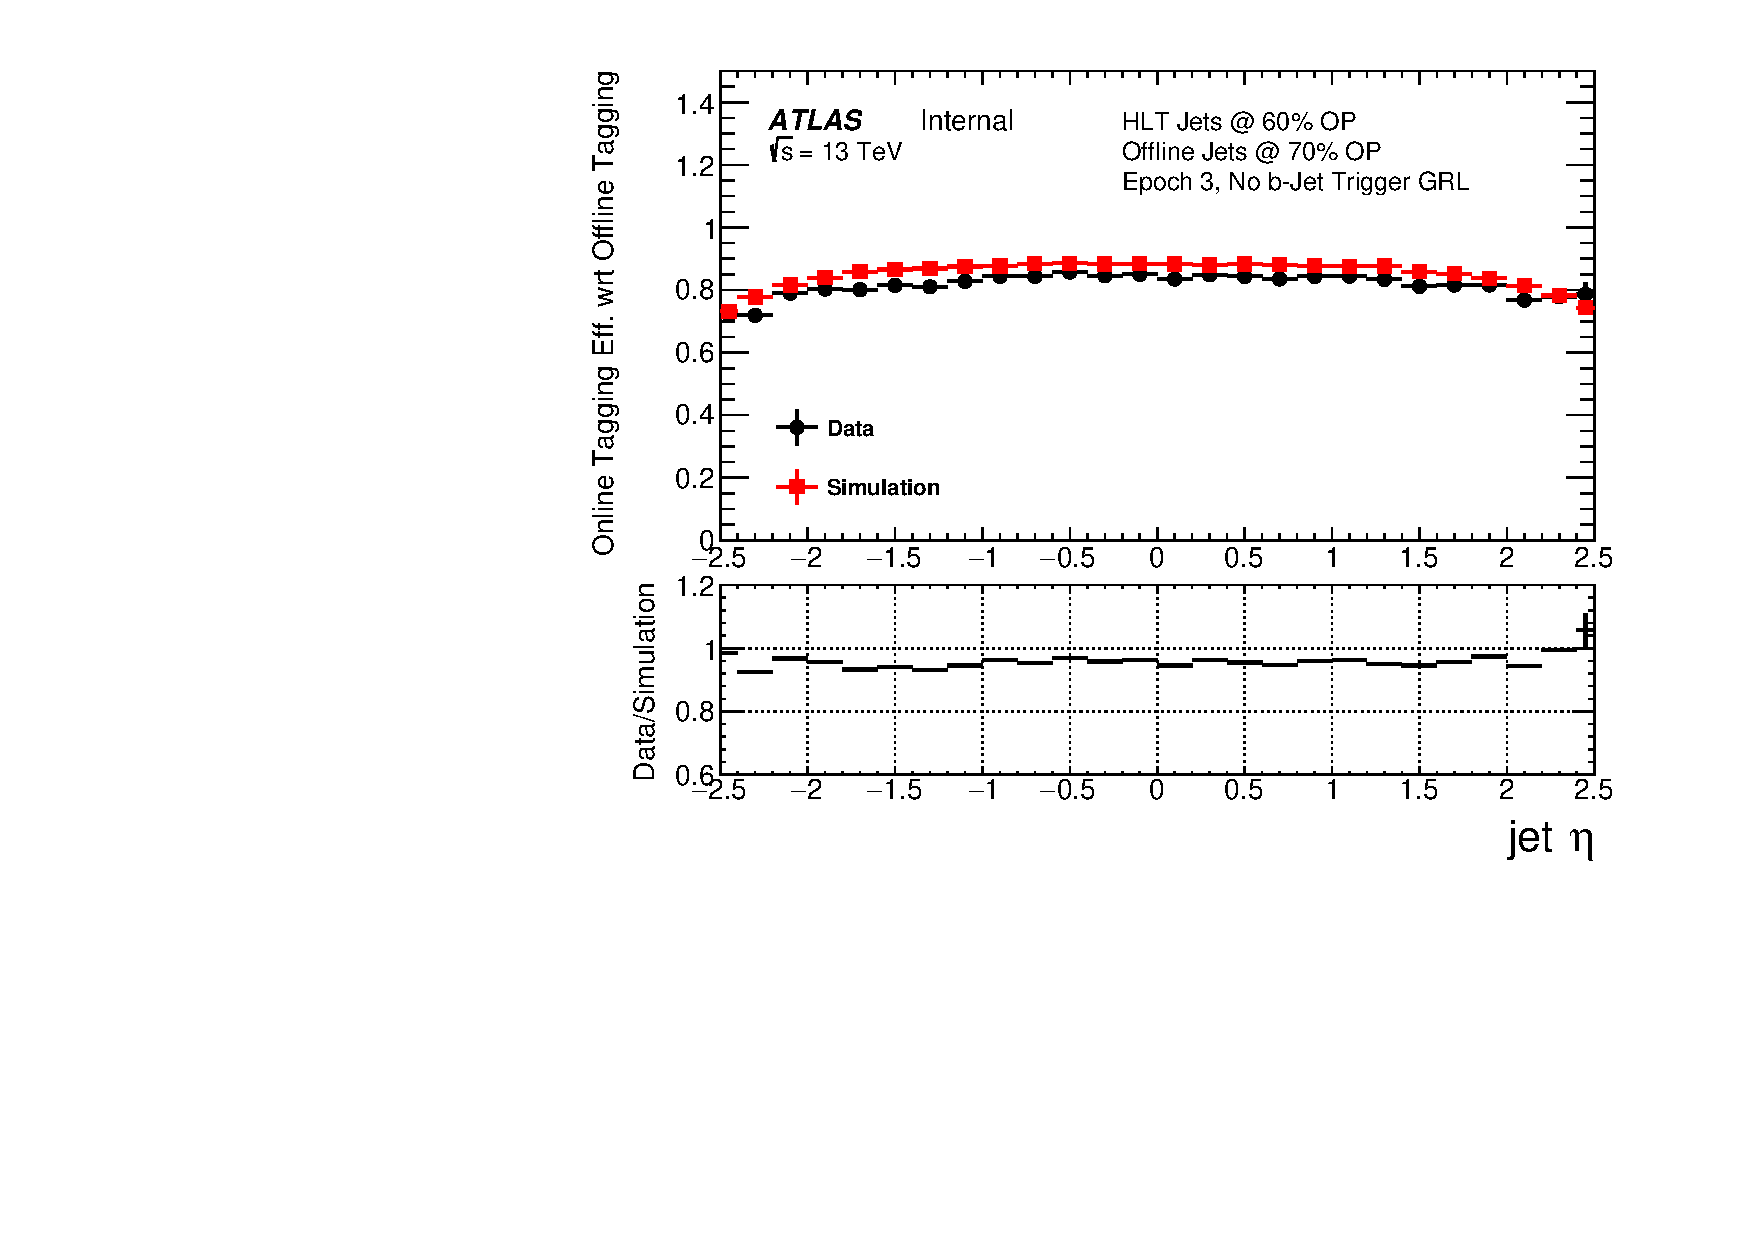
\includegraphics[width=0.47\linewidth, angle=0]{figs/Trigger/Epoch3_noGRL_eff_jetEta.pdf}} \\
  \subcaptionbox{$z_{\,\text{bs}}^{\text{\,online}}$}{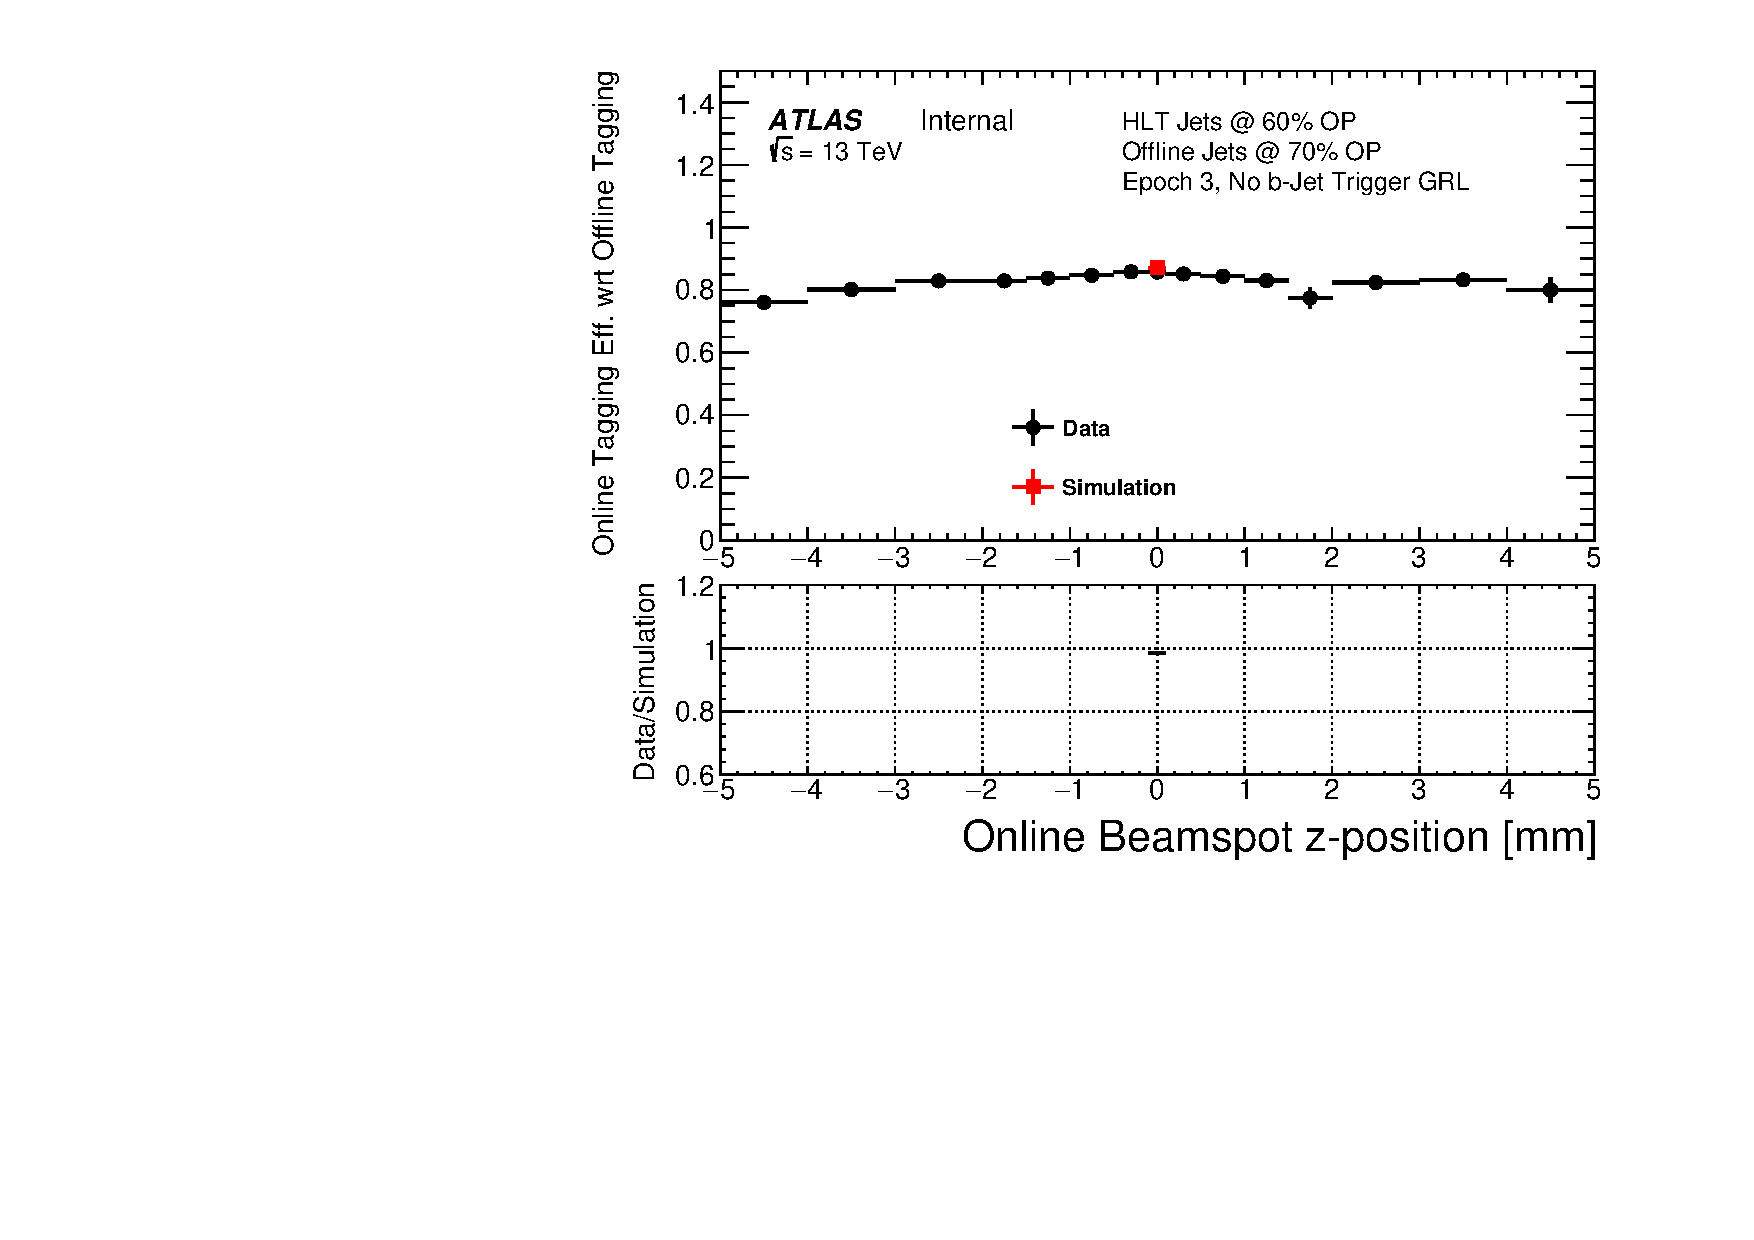
\includegraphics[width=0.47\linewidth, angle=0]{figs/Trigger/Epoch3_noGRL_eff_bs_online_vz.pdf}}
  \subcaptionbox{Vertex Class}{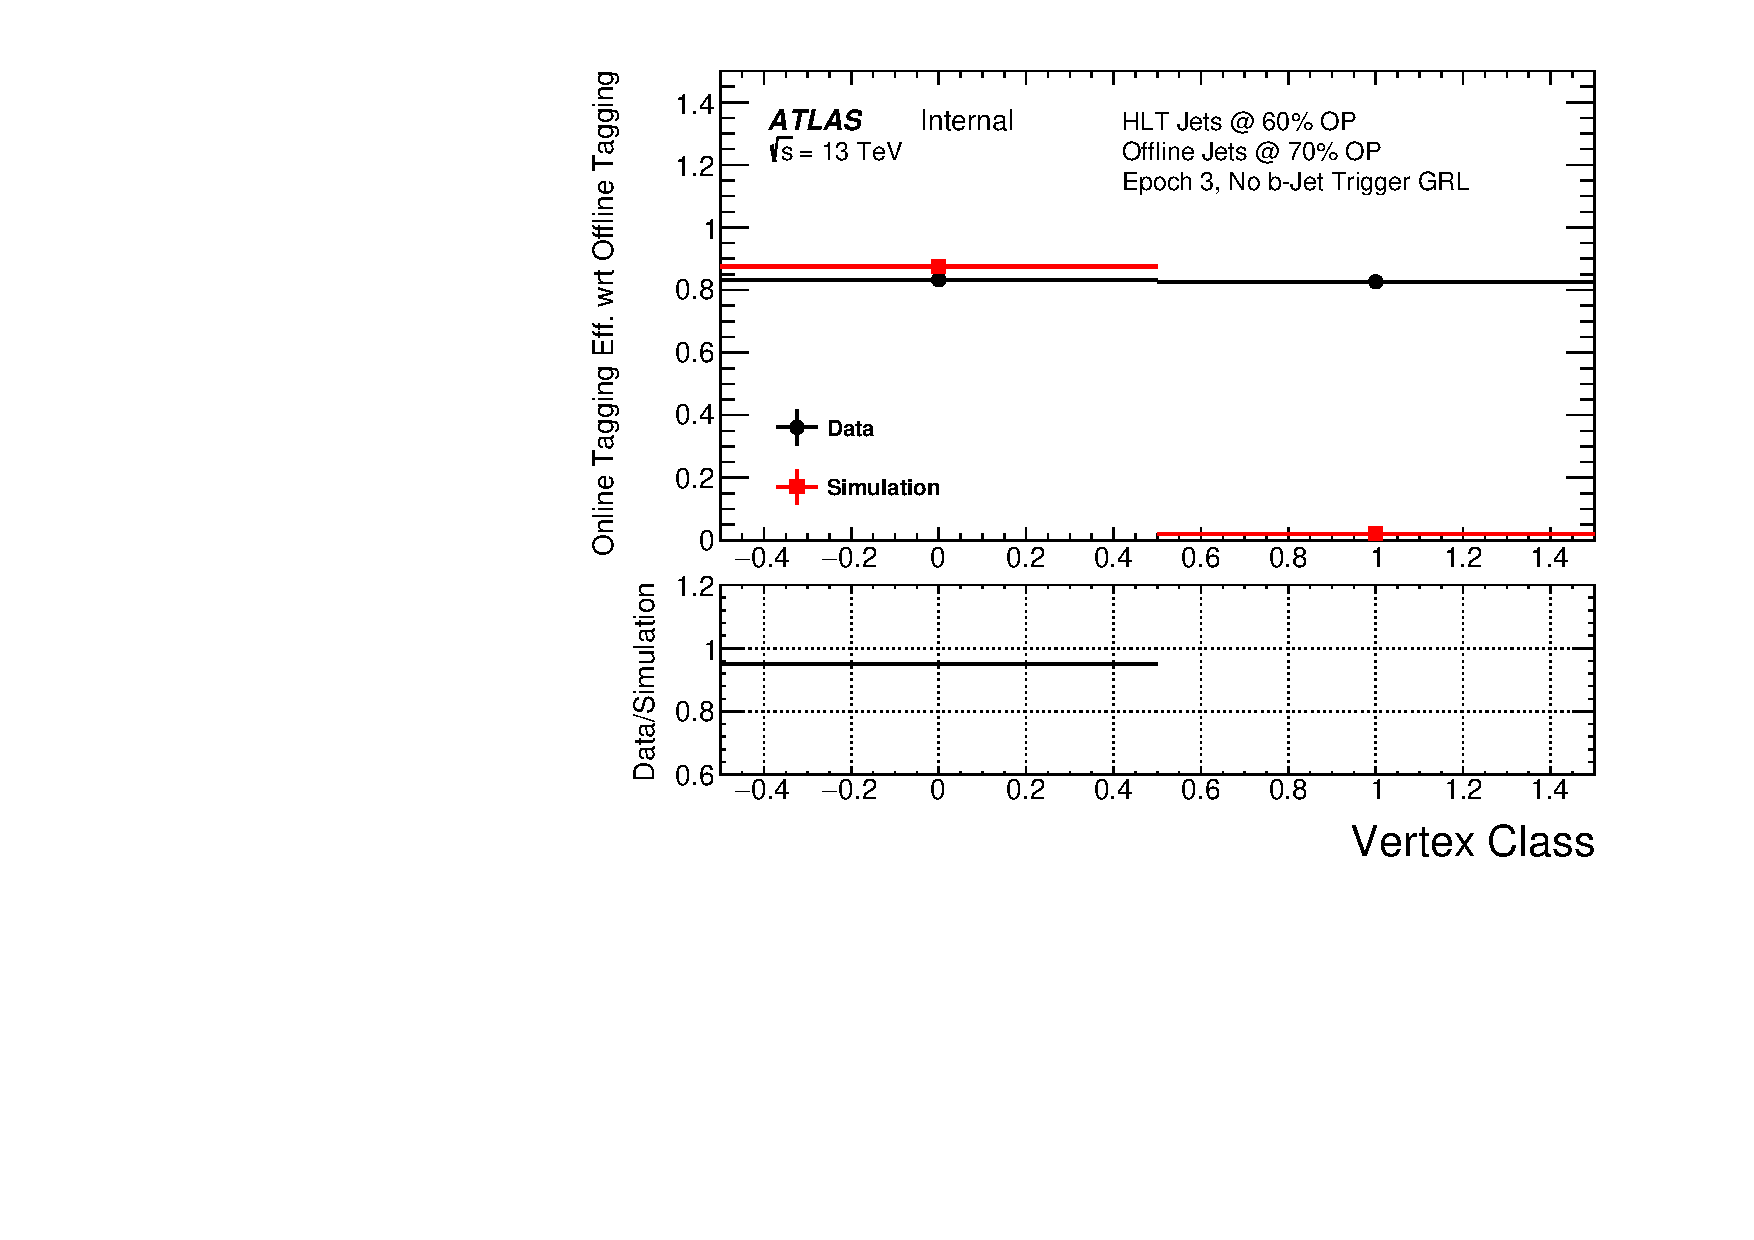
\includegraphics[width=0.47\linewidth, angle=0]{figs/Trigger/Epoch3_noGRL_eff_vtxClass.pdf}}
\end{center}
\vspace{-1em}
%\caption{The 60\% operating point $b$-jet trigger efficiency with respect to the offline 70\% operating point
%  for data from Epoch~3 (black) and simulation (red) against (a) jet-\pT{} and (b) vertex class.
%  Vertex class is defined as 0 when a \textit{xPrmVtx} vertex is found and 1 if not.
%}
\caption[  The $b$-jet trigger efficiency for data from Epoch~3 and simulation.]
        {
          The 60\% operating point $b$-jet trigger efficiency with respect to the offline 70\% operating point
          for data from Epoch~3 (black) and simulation (red) against (a) jet-\pT, (b) jet-$\eta$,
          (c) online beamspot $z$-position and (d) vertex class.
          Vertex class is defined as 0 when a \textit{xPrmVtx} vertex is found and 1 if not.}
\label{fig:Epoch3_eff}
\end{figure}

To summarise, it is shown that at large values of absolute online beamspot $z$-position
the measured $b$-jet trigger efficiency in Epoch~1 and $b$-jet performance efficiency in Epoch~2 is lower in data than in simulation
due to poor \verb|xPrmVtx| PV finding performance.
In Epoch~3 there is reasonable data/simulation agreement due to the use of a backup vertex finding algorithm. 

\newpage
\subsection{$b$-Jet Trigger Aware Good Run List (GRL)}
\label{sec:trig-grl}

To resolve the large data-simulation discrepancies shown in the previous section,
a $b$-jet trigger aware GRL is applied to remove events with $|z_{\,\text{bs}}^{\text{\,online}}| >$ 2mm in Epoch~1 and 2,
such that the events with low efficiency are removed. No such requirement is necessary for Epoch~3 due to the use of a backup primary vertex finding algorithm.
To retain as much data as possible, the cut value is chosen be the widest value of $|z_{\,\text{bs}}^{\text{\,online}}|$
that corresponds to an efficiency not significantly reduced by the \verb|xPrmVtx| algorithm performance issue.
A \SI{2}{\mm} cut is selected using Figure~\ref{fig:Epoch1_eff}(b) and Figure~\ref{fig:Epoch2_bperf}(b).

It was decided to use a $b$-jet trigger aware GRL instead of deriving a correction factor for the full data-set.
The cost of using a $b$-jet trigger aware GRL is a reduction in the integrated luminosity of the data-set from  32.9~\ifb{} to 24.3~\ifb.
The reasons for using a $b$-jet trigger aware GRL are threefold.
Firstly, as there is no online beamspot position distribution in simulation it is not clear that kinematics of events at high  $z_{\,\text{bs}}^{\text{\,online}}$ can be well understood and modelled;
the sculpting of the efficiency with respect to jet-$\eta$ shown in Figure~\ref{fig:Epoch2_bperf}(c) is an example of this.
Secondly, the efficiencies are quite low at high beamspot $z$-position,
so the loss in luminosity x acceptance is relatively small.
Finally, using a GRL means that the stated value of integrated luminosity is a more accurate representation of the size of the data-set.

The application of the GRL significantly improves data-simulation agreement in Epoch~1 and 2.
Figure~\ref{fig:Epoch1_bslt2mm_eff} shows that the $b$-jet trigger efficiency for Epoch~1 becomes approximately 90-95\% of the efficiency measured in simulation.
Figure~\ref{fig:Epoch2_bslt2mm_bperf} shows that the \mbox{$b$-performance} trigger efficiency measured in Epoch~2 becomes approximately 95\% of the efficiency in simulation.

\begin{figure}[!htb]
  \begin{center}
    \captionsetup[subfigure]{aboveskip=0pt,justification=centering}
    \subcaptionbox{Jet-\pT}{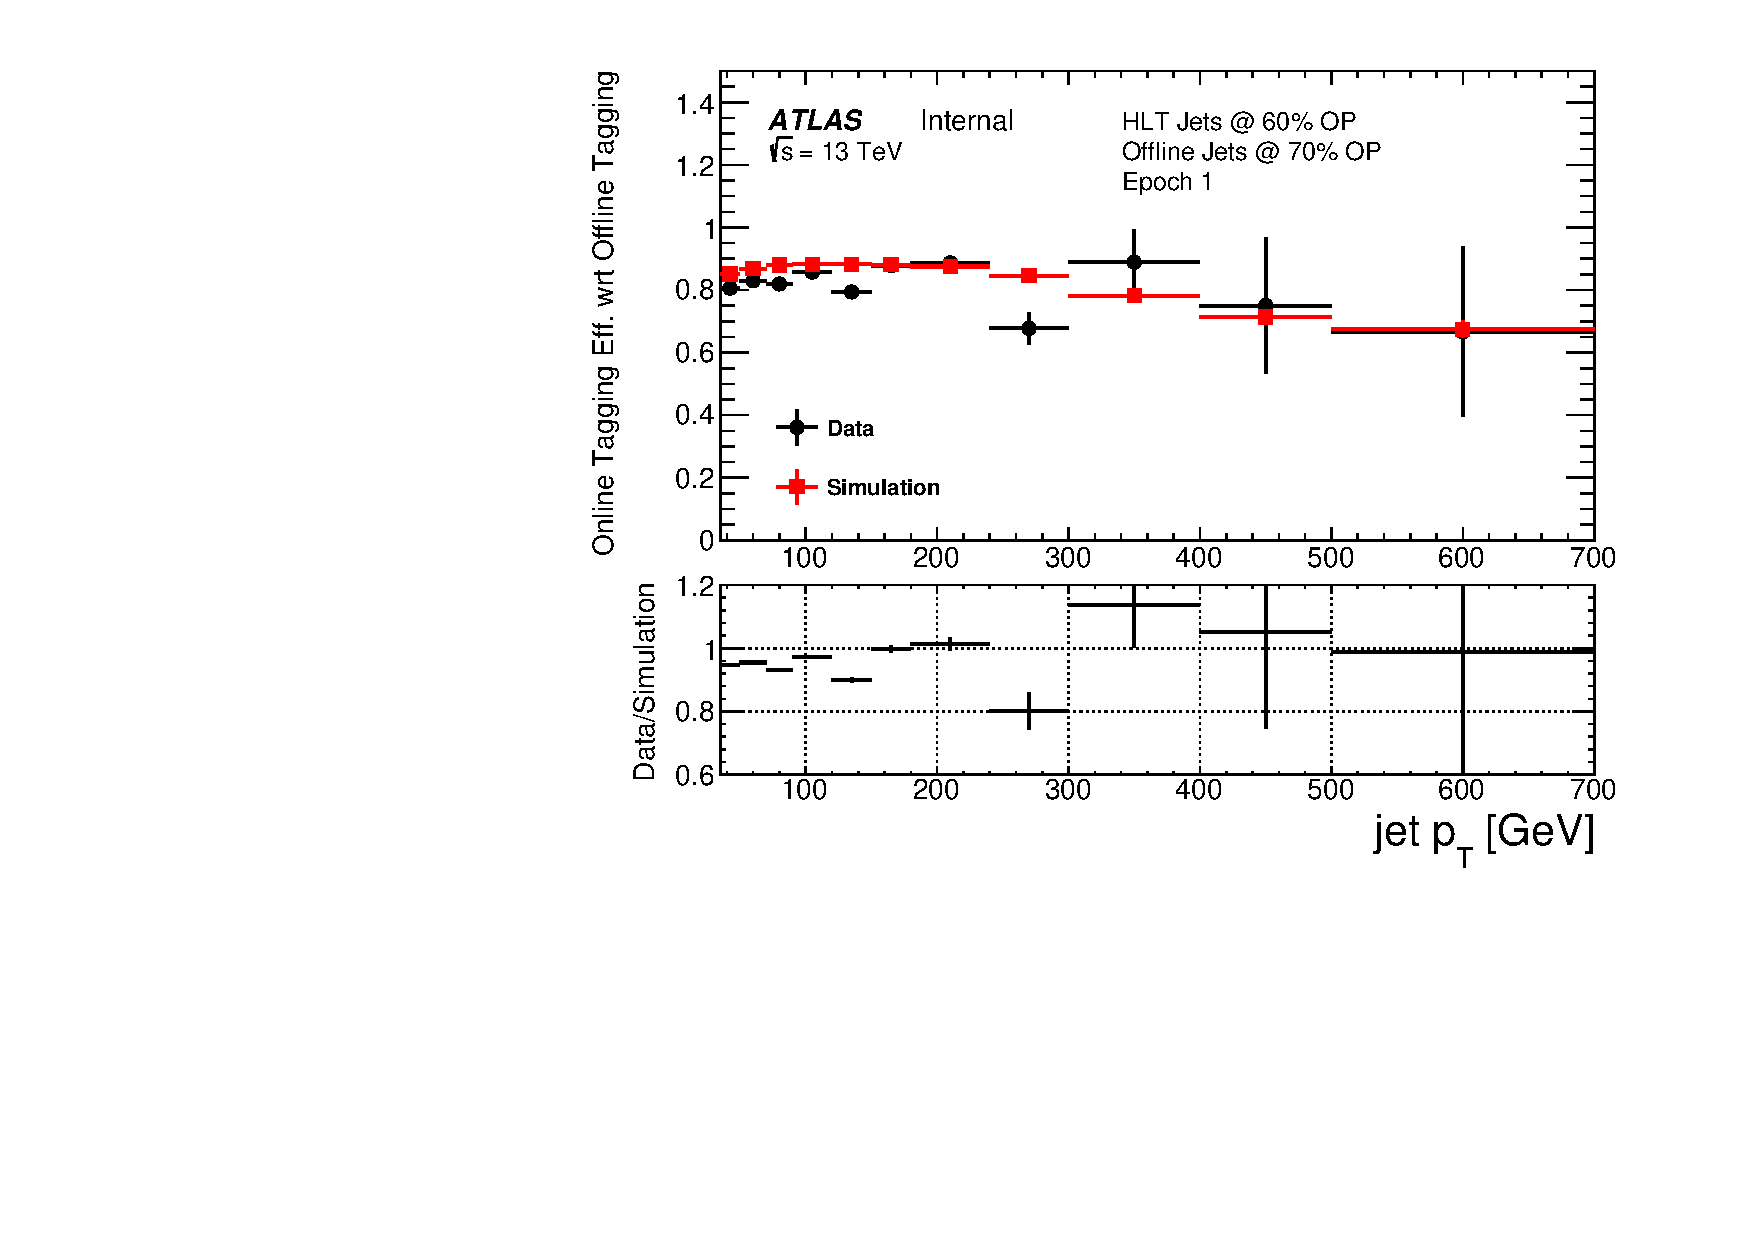
\includegraphics[width=0.47\linewidth, angle=0]{figs/Trigger/Epoch1_GRL_bslt2mm_eff_jetPt.pdf} }
    \subcaptionbox{Jet-$\eta$}{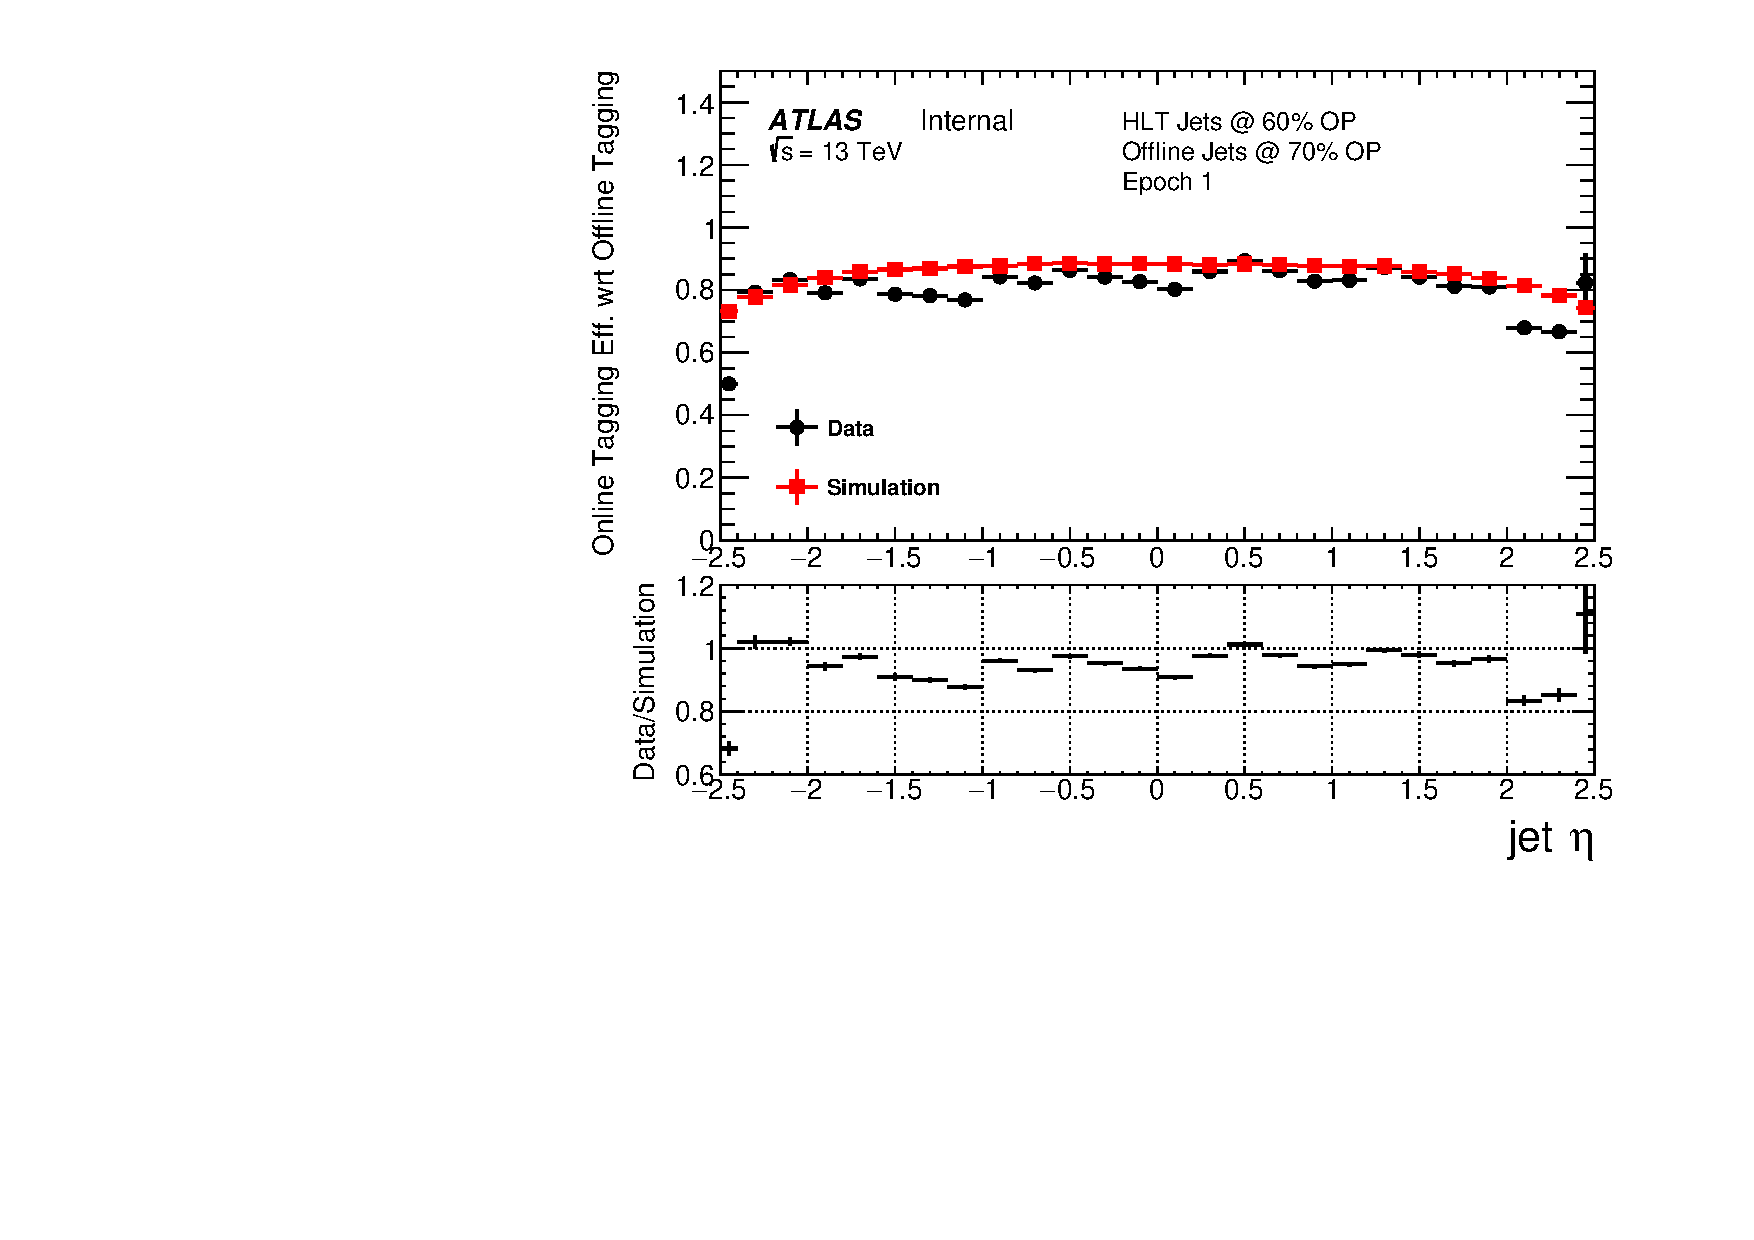
\includegraphics[width=0.47\linewidth, angle=0]{figs/Trigger/Epoch1_GRL_bslt2mm_eff_jetEta.pdf}}
  \end{center}
\vspace{-1em}
  \caption[
  The $b$-jet trigger efficiency for data from Epoch~2 and for simulated events.
  The $b$-jet trigger aware GRL has been applied.
]
        {The 60\% operating point $b$-jet trigger efficiency with respect to the offline 70\% operating point
    for data from Epoch~1 (black) and simulation (red) against (a)~jet-\pT{} and (b)~jet-$\eta$.
    The $b$-jet trigger aware GRL has been applied.}
  \label{fig:Epoch1_bslt2mm_eff}
\end{figure}

\begin{figure}[!htb]
  \begin{center}
    \captionsetup[subfigure]{aboveskip=0pt,justification=centering}
    \subcaptionbox{Leading jet-\pT}{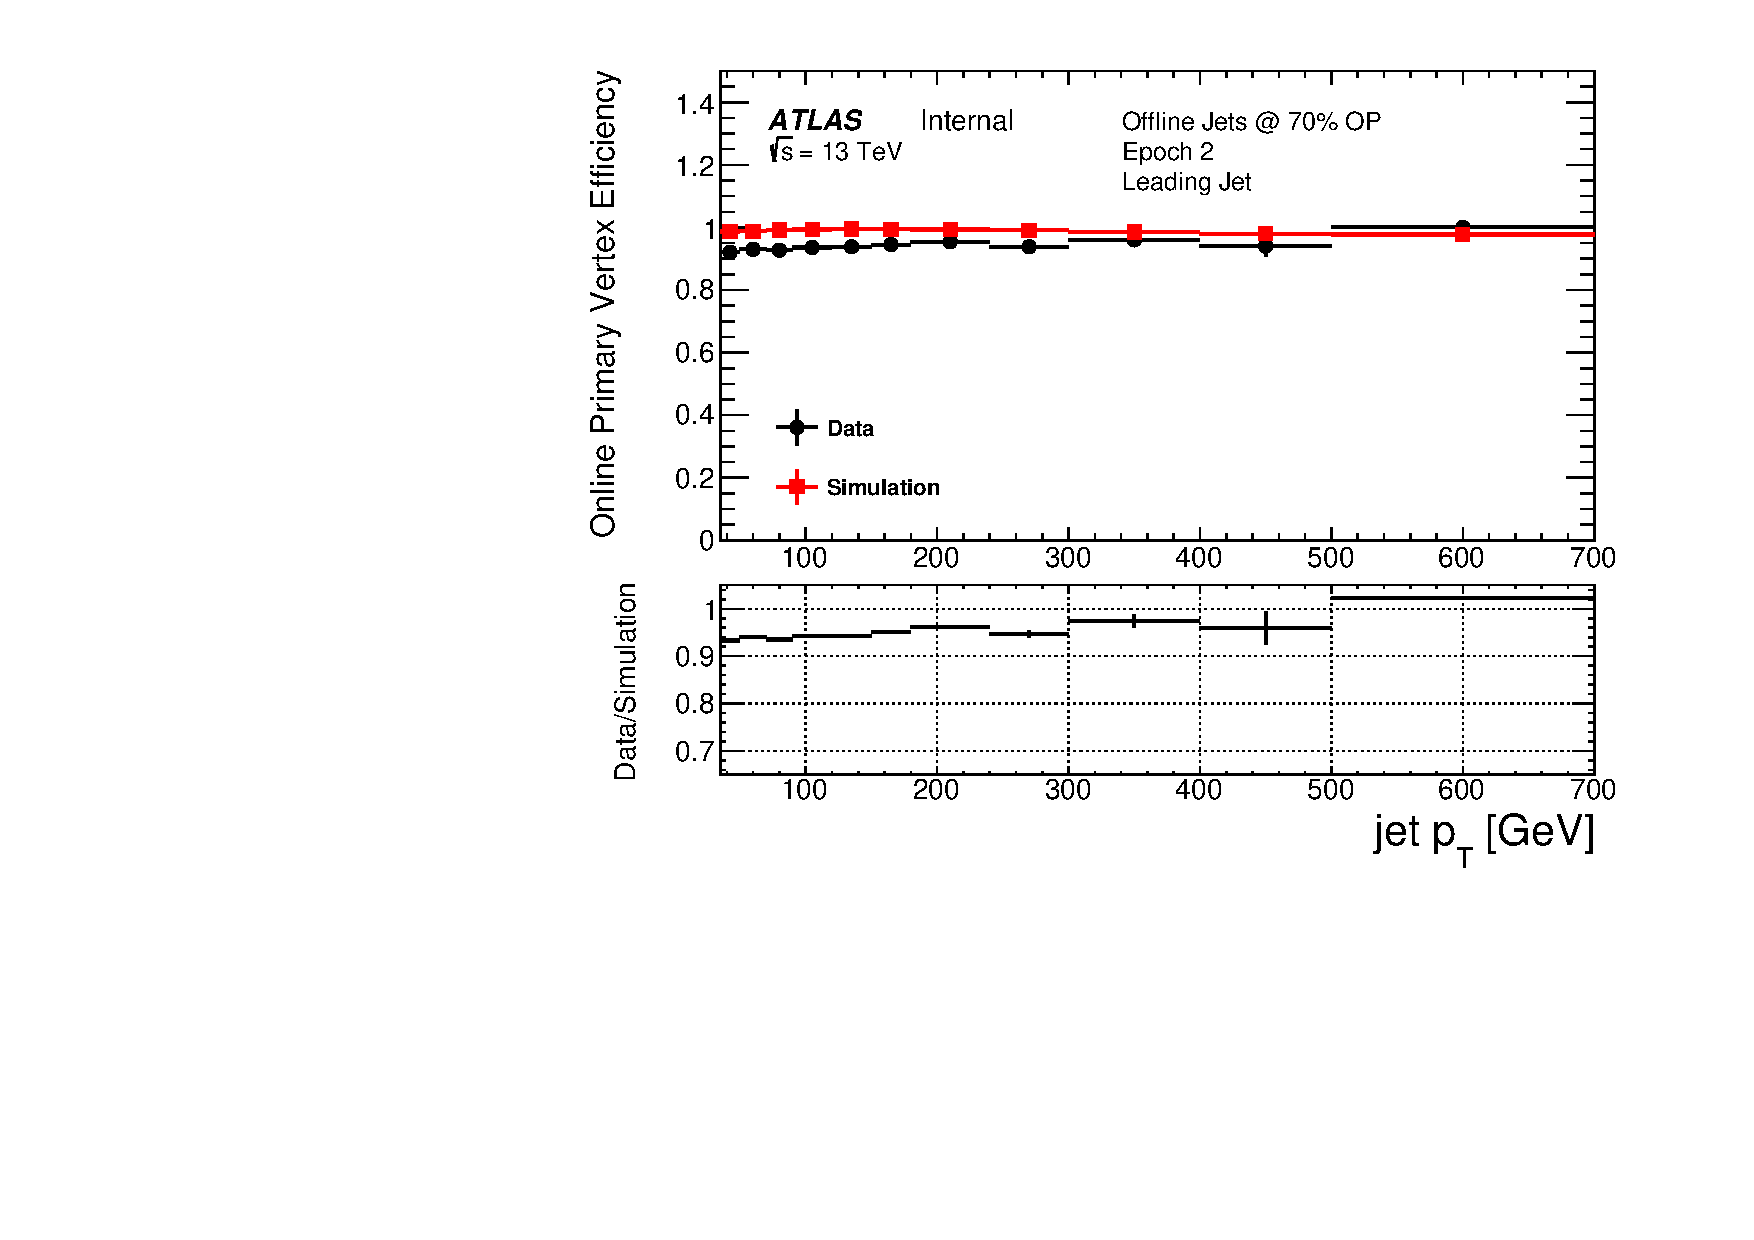
\includegraphics[width=0.47\linewidth, angle=0]{figs/Trigger/Epoch2_GRL_bslt2mm_bPerfEff_leadingJet_jetPt.pdf} }
    \subcaptionbox{Leading jet-$\eta$}{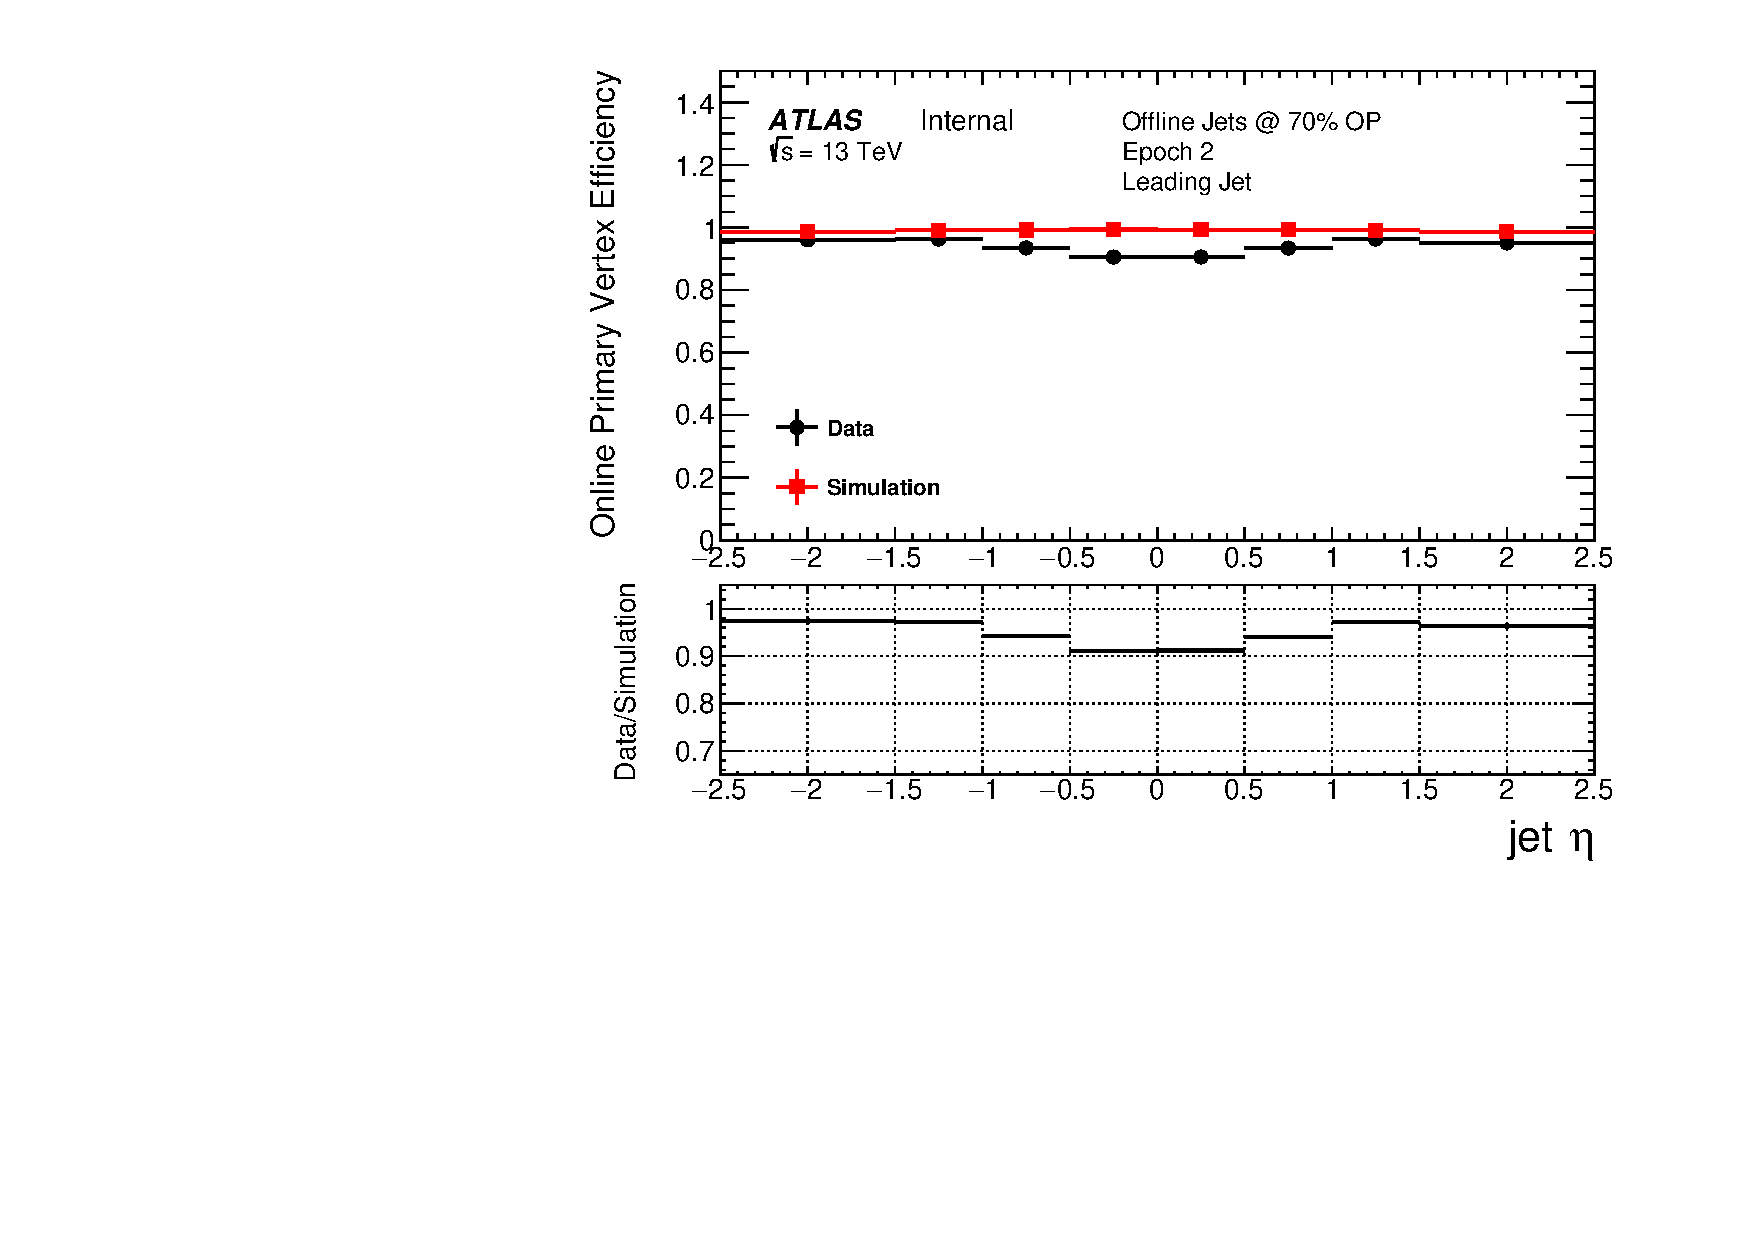
\includegraphics[width=0.47\linewidth, angle=0]{figs/Trigger/Epoch2_GRL_bslt2mm_bPerfEff_leadingJet_jetEta.pdf}}
  \end{center}
\vspace{-1em}
  \caption[
    The online primary vertex efficiency for data in Epoch~2 and for simulated events.
    The $b$-jet trigger aware GRL has been applied.
  ]
        {The online primary vertex efficiency, $\epsilon_{\text{PV}}$, for data from Epoch~2 (black) and simulation (red) against leading (a) jet-\pT~and (b) jet-$\eta$.
    The $b$-jet trigger aware GRL has been applied.}
  \label{fig:Epoch2_bslt2mm_bperf}
\end{figure}

Figures~\ref{fig:Full_bslt2mm_eff}~and~\ref{fig:Full_bslt2mm_bperf} show the measured
$b$-jet trigger efficiency and online primary vertex efficiency
for the full 2016 data-set, combining Epochs 1, 2 and 3,
with the $b$-jet trigger aware GRL applied.
Data agrees with simulation within 5\%.  A residual kinematic bias with respect to leading jet-$\eta$ is still present.
%This represents the raw observed data/simulation efficiencies when the full event selection has been applied.

\begin{figure}[!ht]
  \begin{center}
    \captionsetup[subfigure]{aboveskip=0pt,justification=centering}
    \subcaptionbox{Jet-\pT}{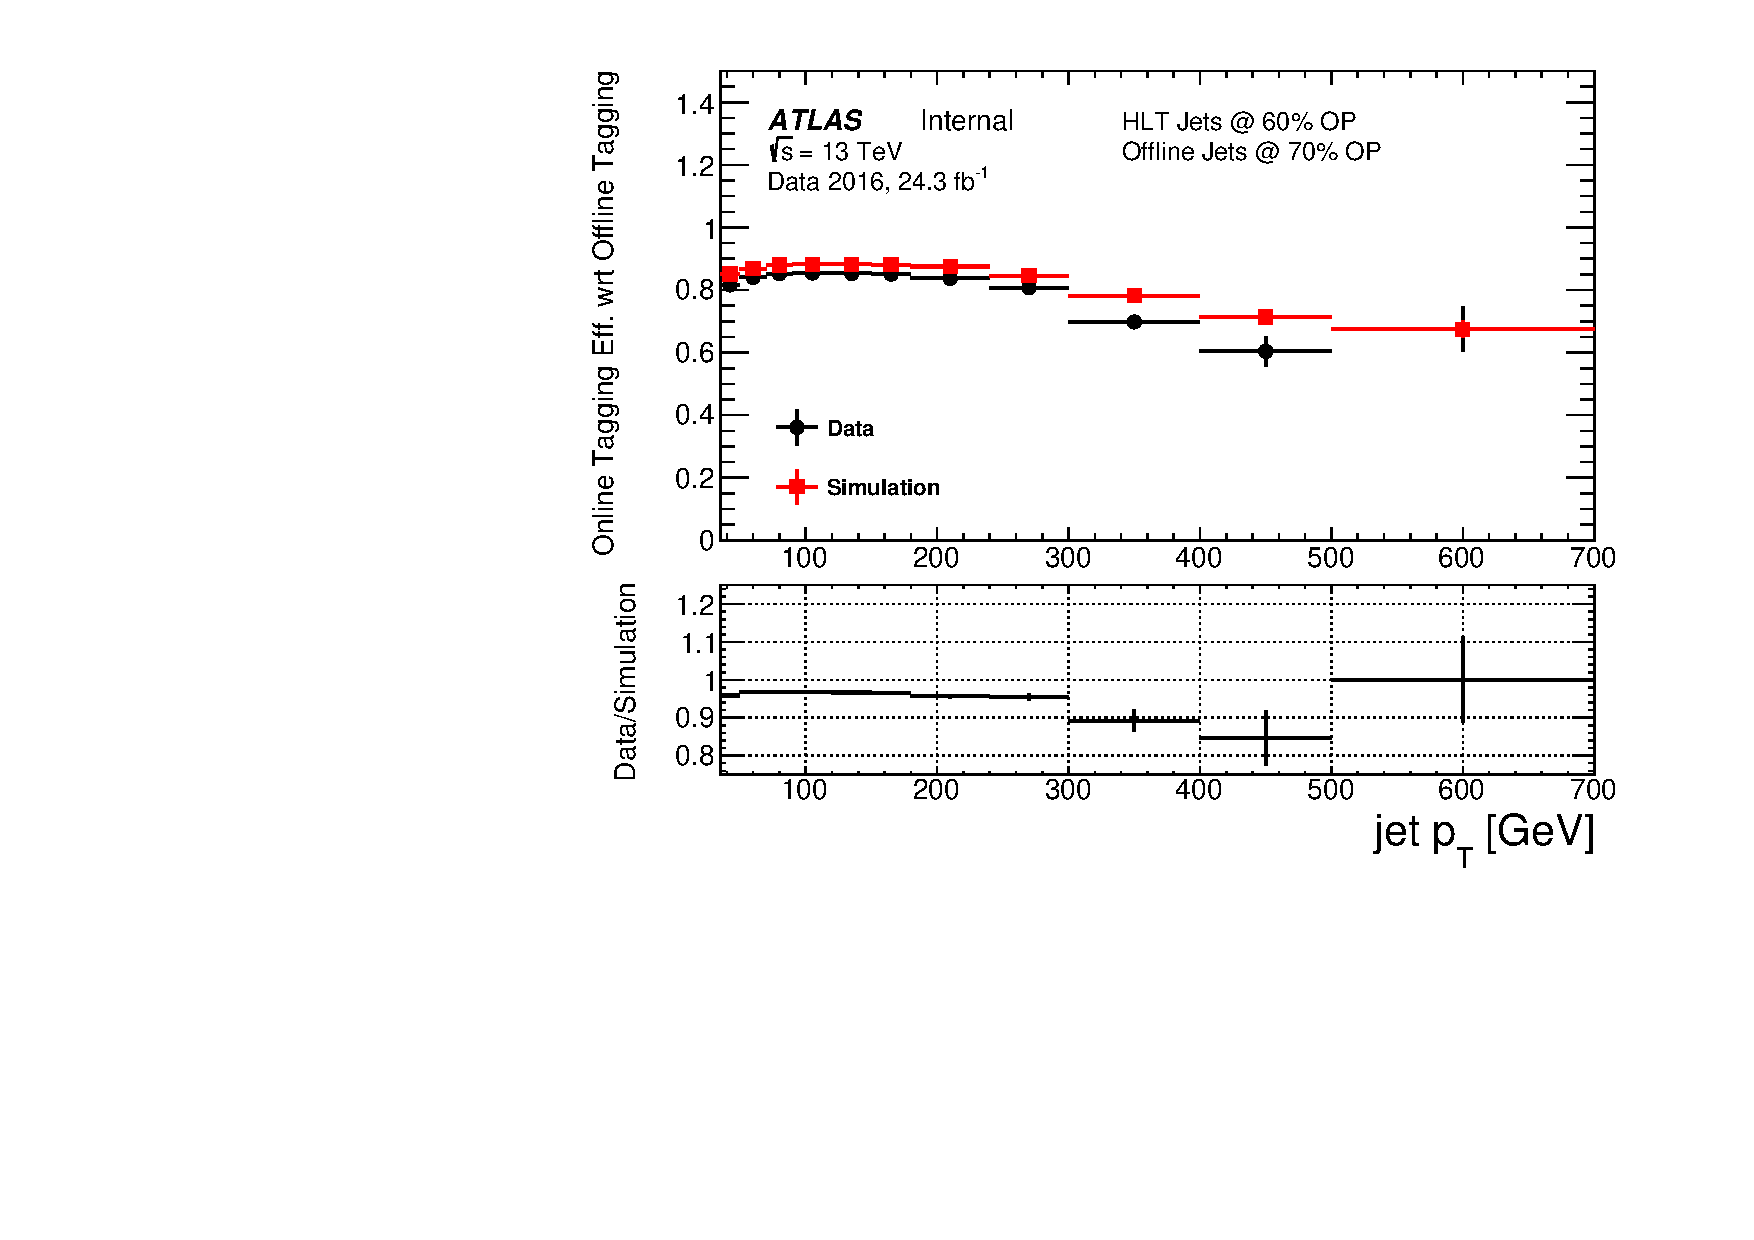
\includegraphics[width=0.47\linewidth, angle=0]{figs/Trigger/Full_GRL_bslt2mm_eff_jetPt.pdf}}
    \subcaptionbox{Jet-$\eta$}{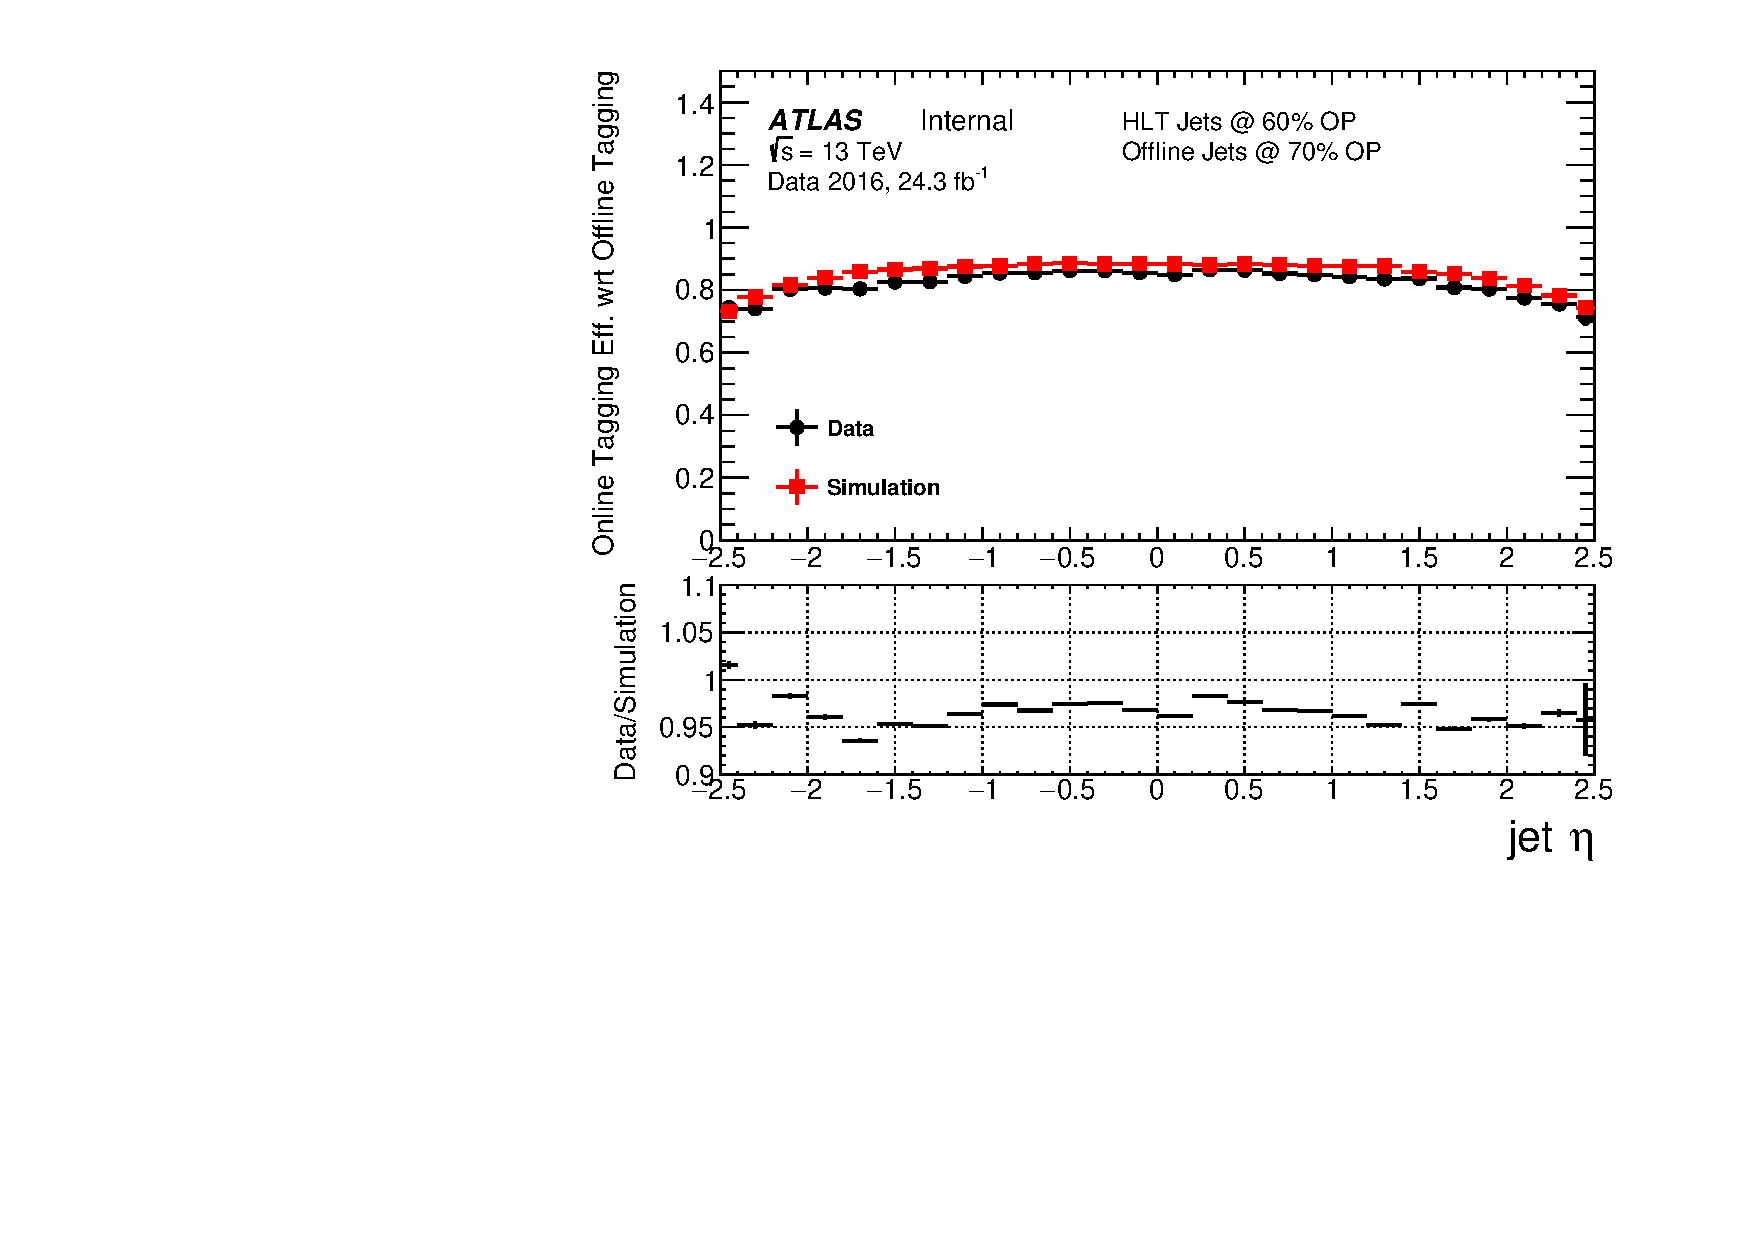
\includegraphics[width=0.47\linewidth, angle=0]{figs/Trigger/Full_GRL_bslt2mm_eff_jetEta.pdf}}\\
    \subcaptionbox{$z_{\,\text{bs}}^{\text{\,online}}$}{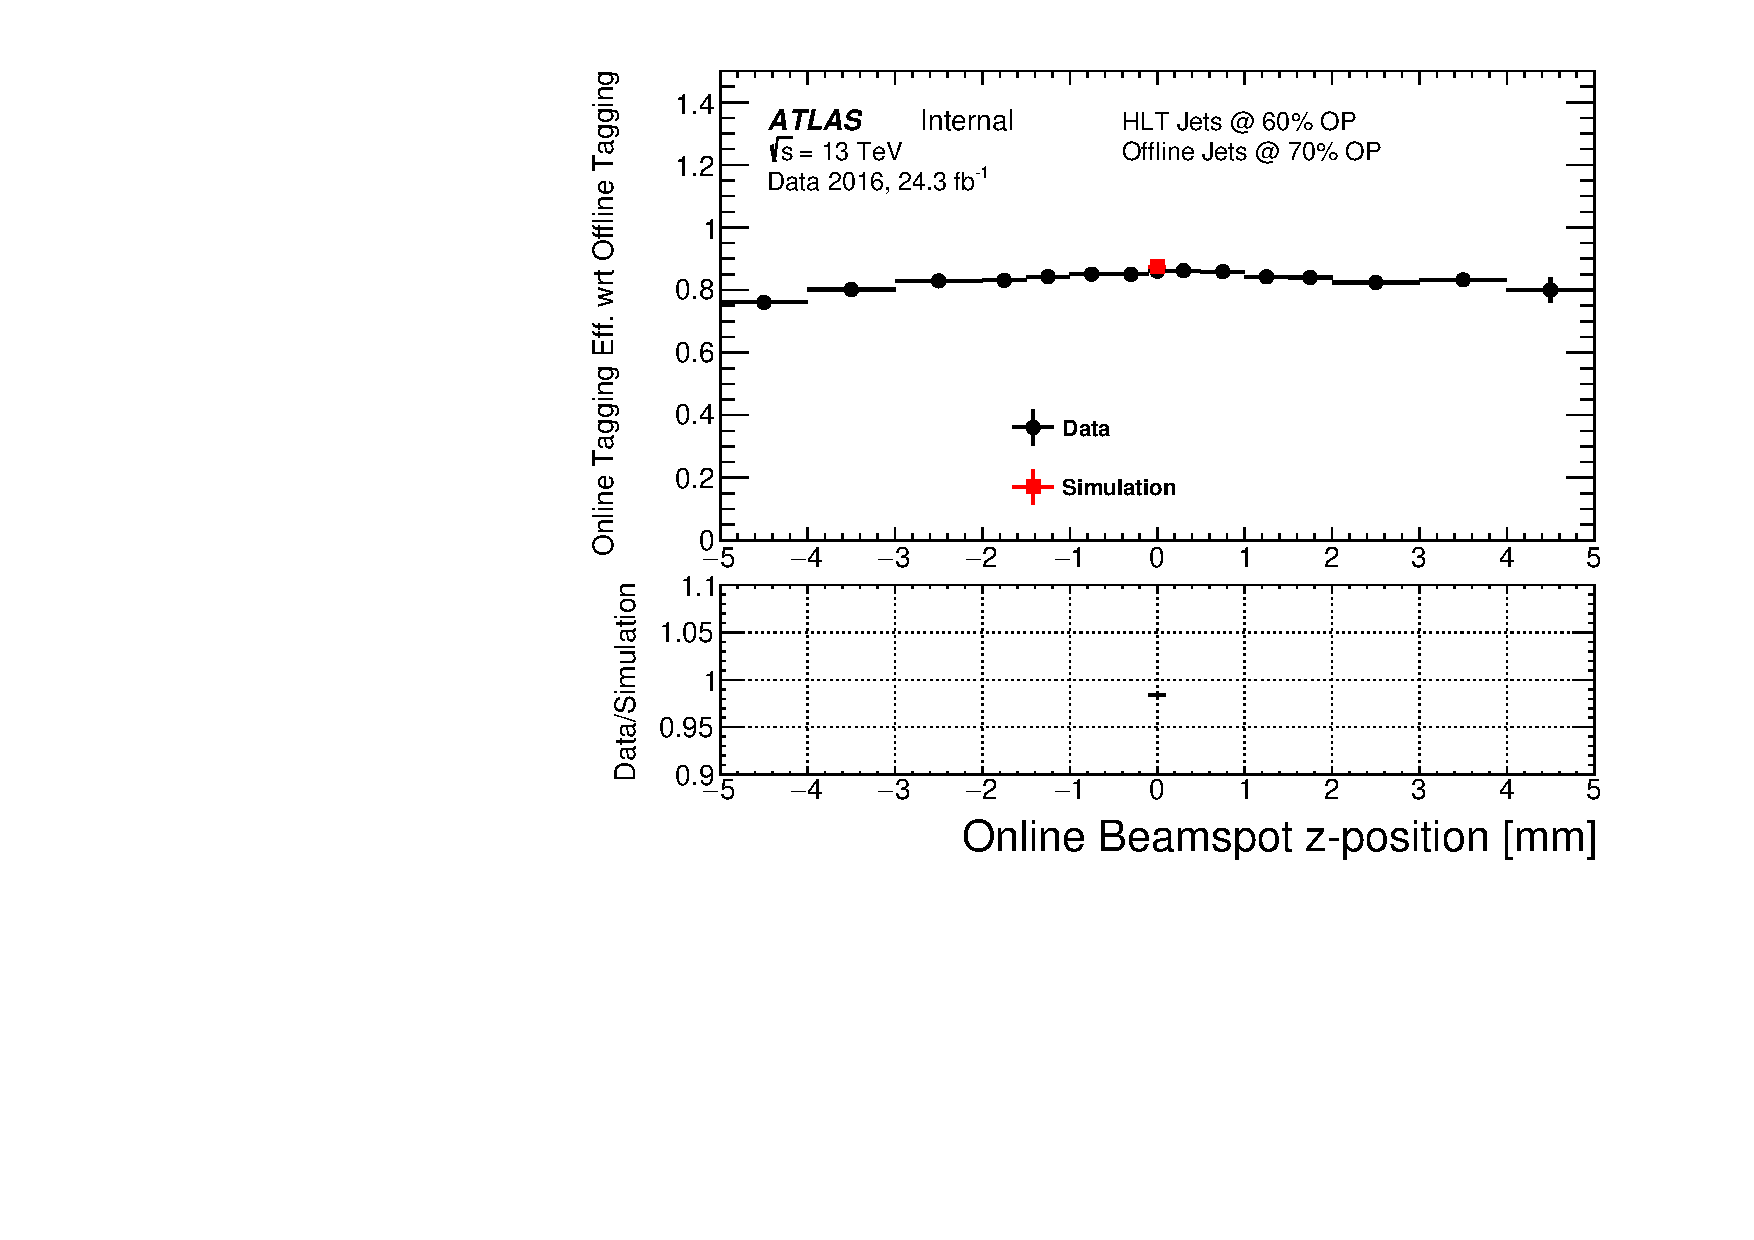
\includegraphics[width=0.47\linewidth, angle=0]{figs/Trigger/Full_GRL_bslt2mm_eff_bs_online_vz.pdf}}
    \subcaptionbox{Vertex Class}{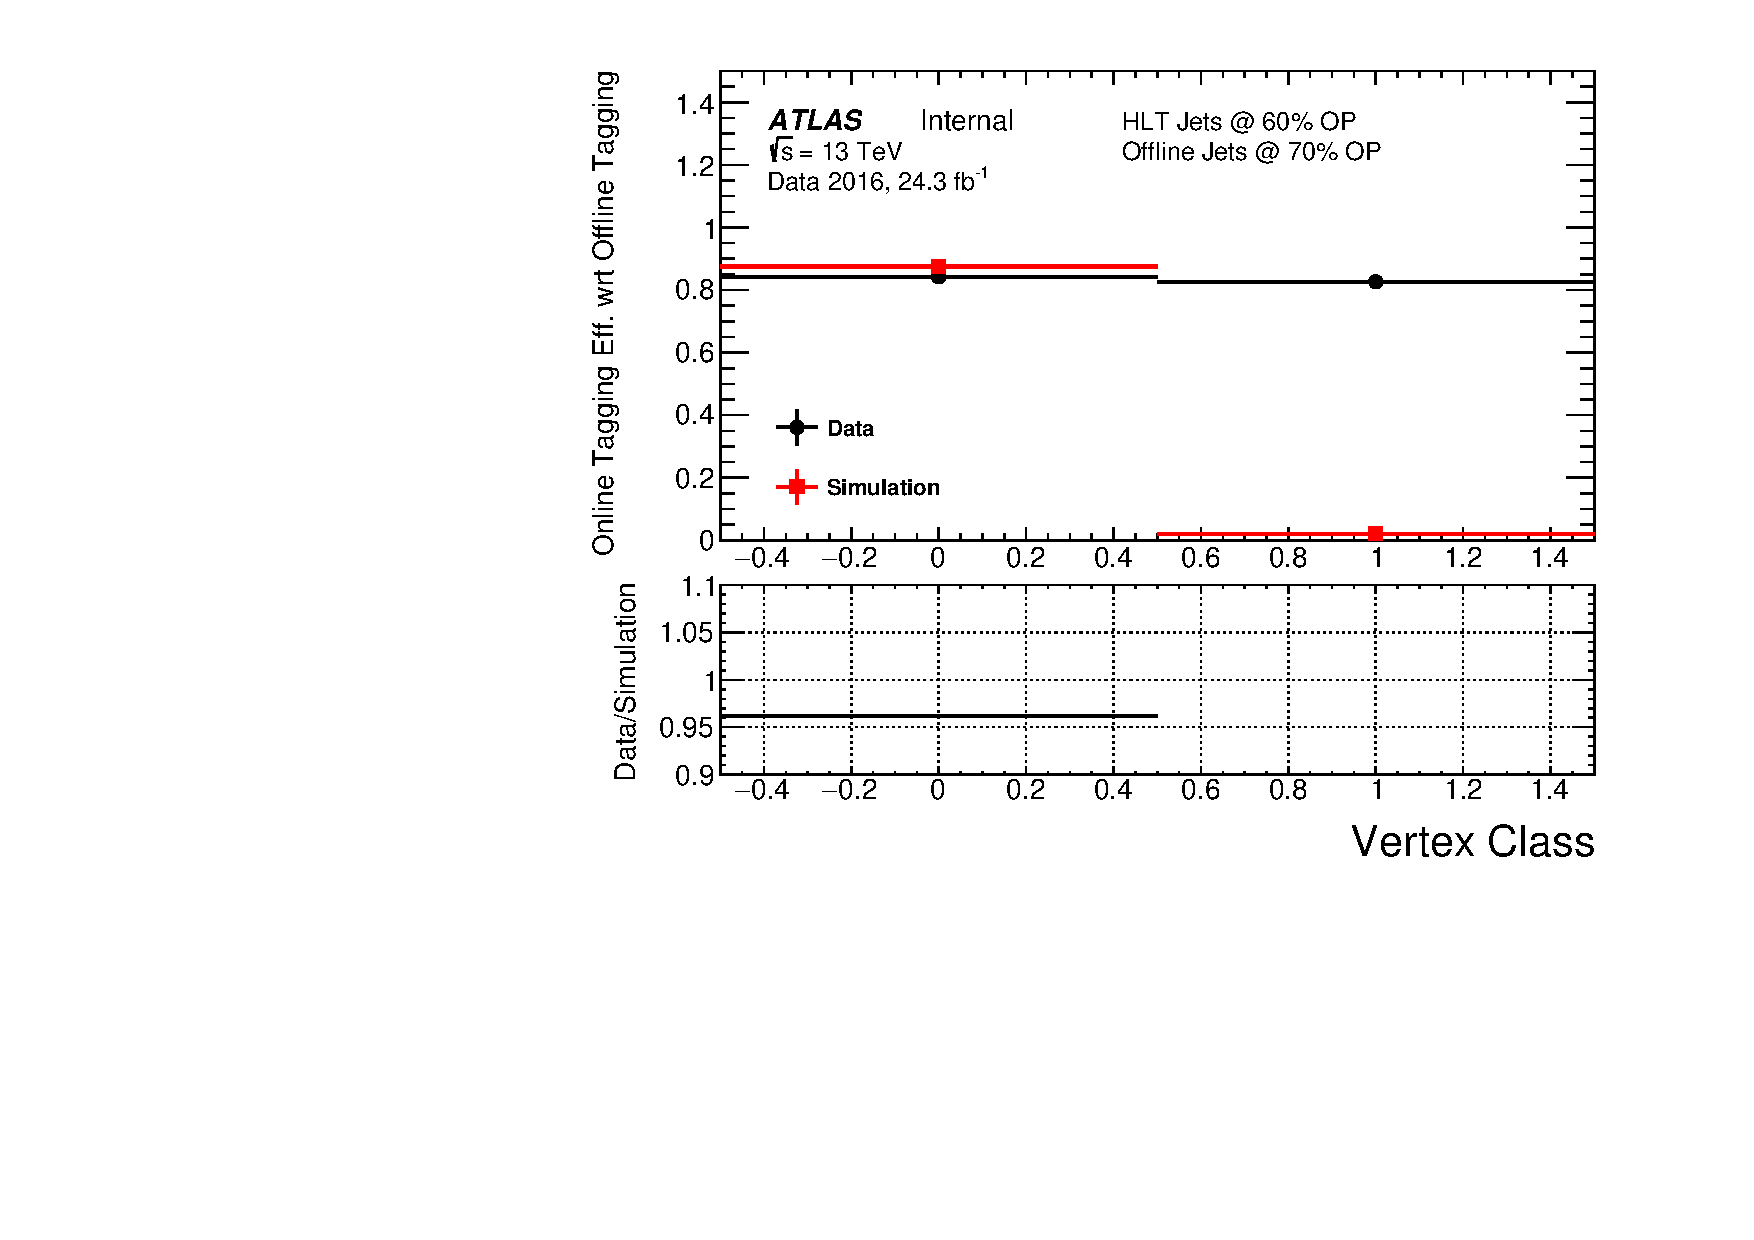
\includegraphics[width=0.47\linewidth, angle=0]{figs/Trigger/Full_GRL_bslt2mm_eff_vtxClass.pdf}}
  \end{center}
\vspace{-1em}
\caption[
  The $b$-jet trigger efficiency for the full 2016 data-set and for simulated events.
  The $b$-jet trigger aware GRL has been applied.
]
        {The 60\% operating point $b$-jet trigger efficiency with respect to the offline 70\% operating point
    for the full 2016 data-set (black) and simulation (red) against (a)~jet-\pT{}, (b)~jet-$\eta$, (c) online beamspot $z$-position and (d) vertex class.
    Vertex class is defined as 0 when a \textit{xPrmVtx} vertex is found and 1 if not.
    The $b$-jet trigger aware GRL has been applied.
}
  \label{fig:Full_bslt2mm_eff}
\end{figure}

\begin{figure}[!ht]
  \begin{center}
    \captionsetup[subfigure]{aboveskip=0pt,justification=centering}
    \subcaptionbox{Leading jet-\pT}{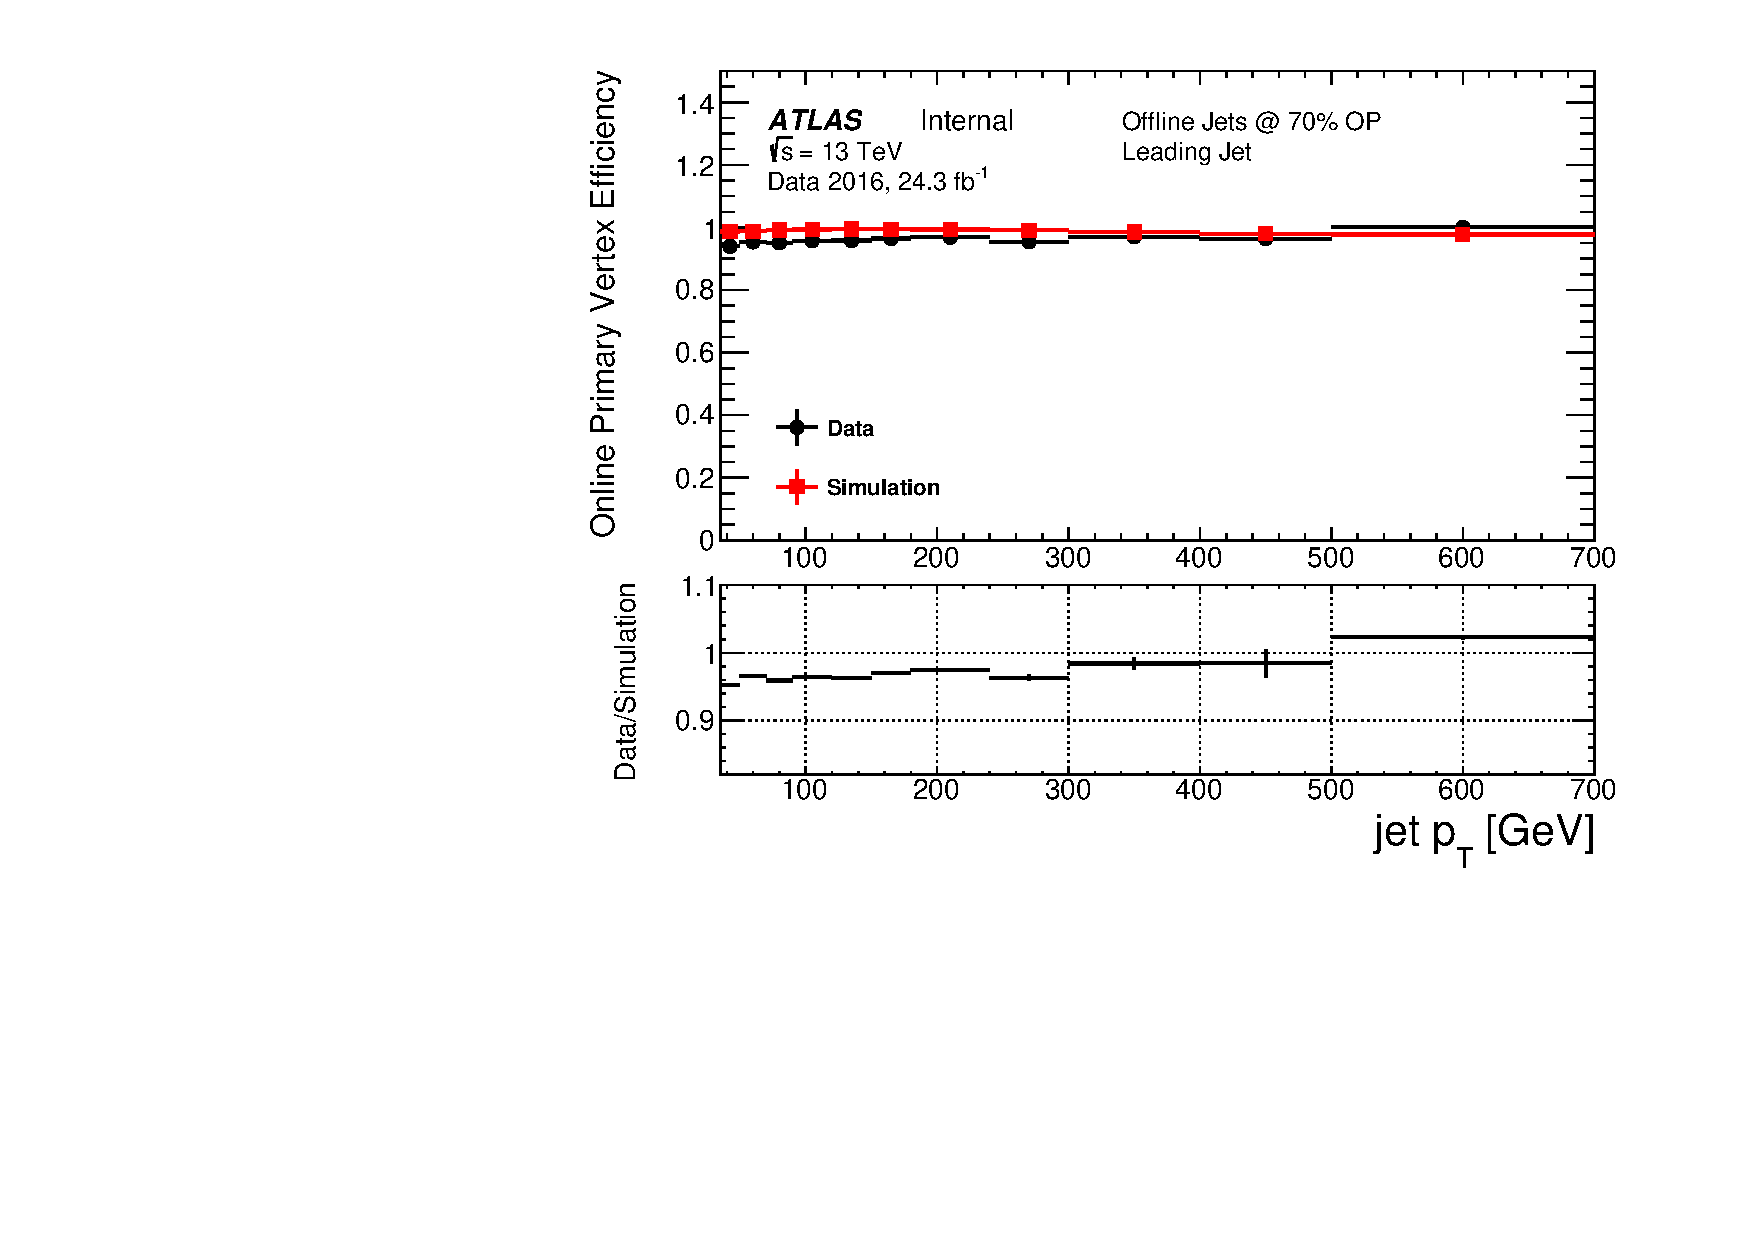
\includegraphics[width=0.47\linewidth, angle=0]{figs/Trigger/Full_GRL_bslt2mm_bPerfEff_leadingJet_jetPt.pdf}}
    \subcaptionbox{Leading jet-$\eta$}{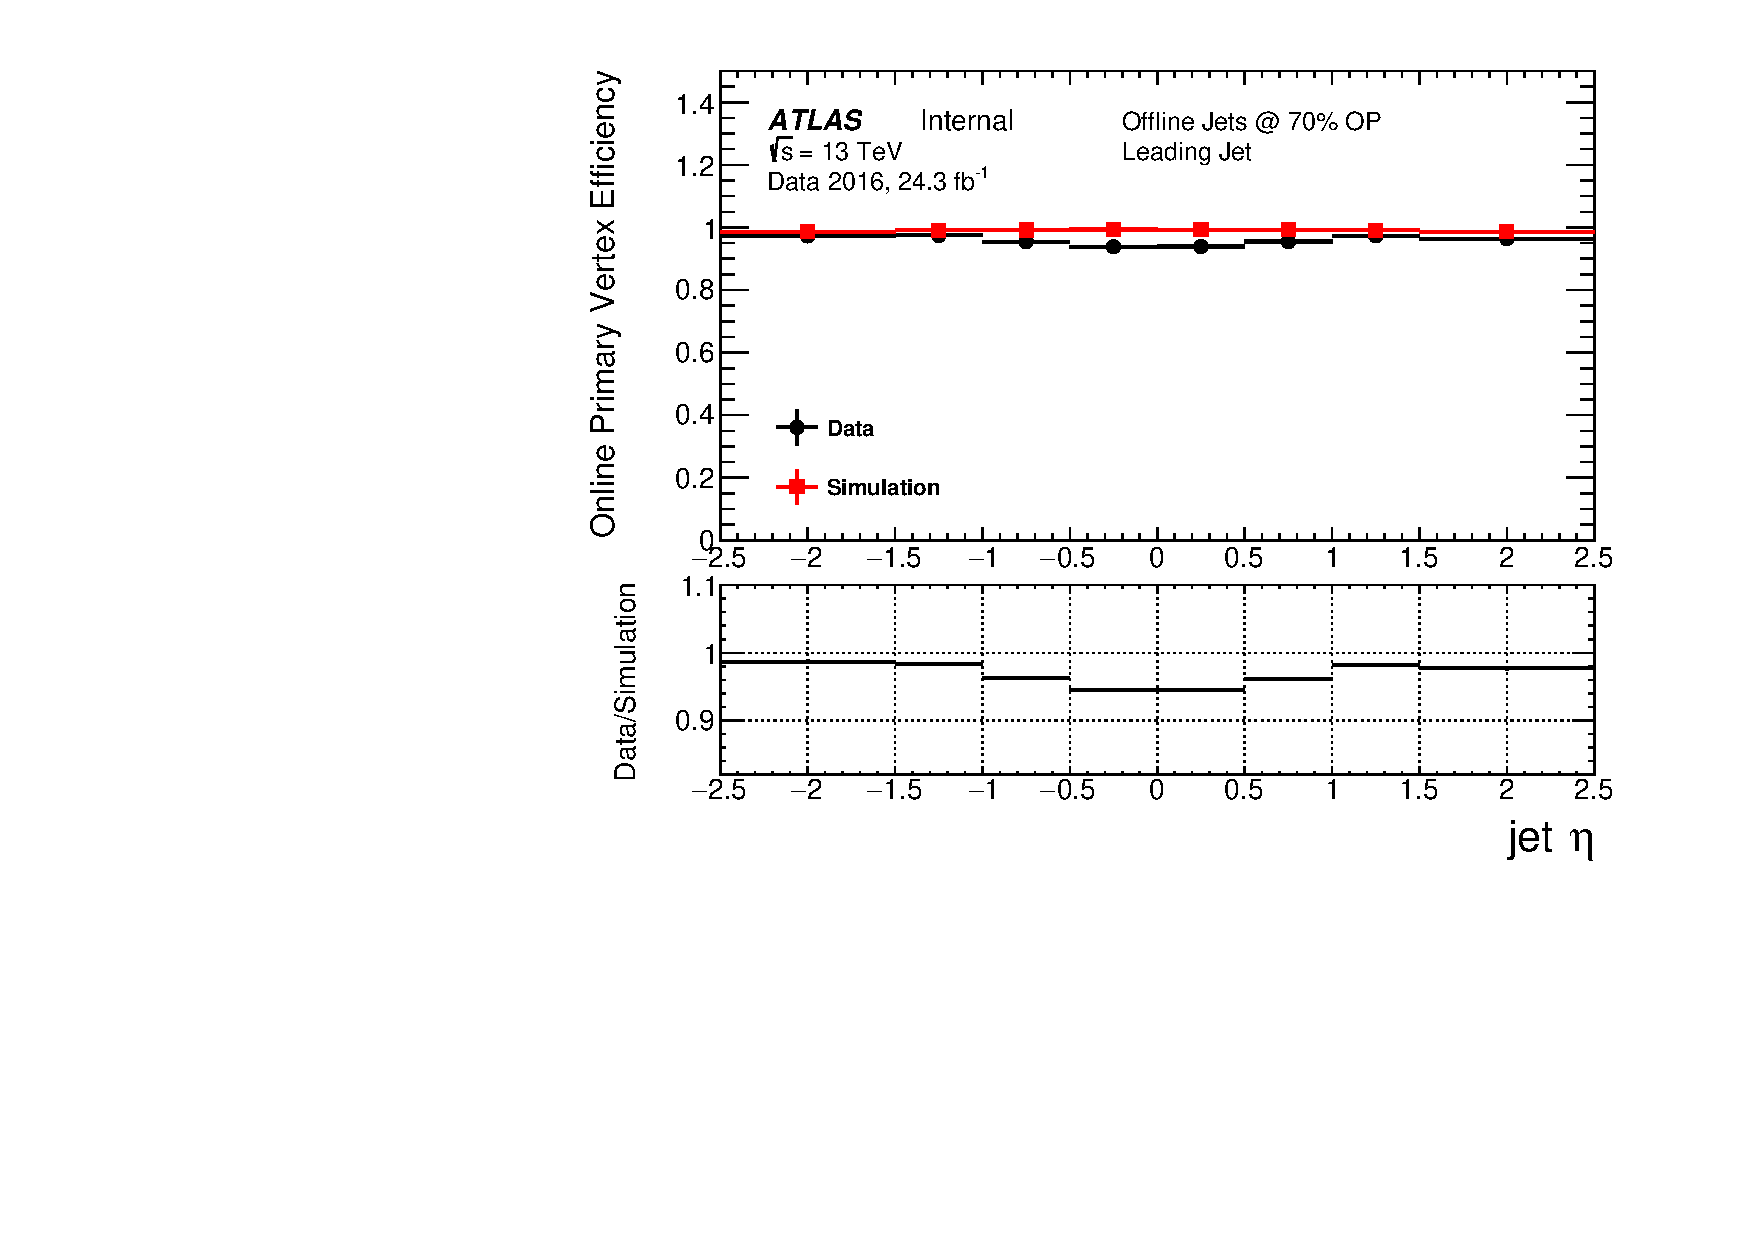
\includegraphics[width=0.47\linewidth, angle=0]{figs/Trigger/Full_GRL_bslt2mm_bPerfEff_leadingJet_jetEta.pdf}}
  \end{center}
\vspace{-1em}
\caption[
  The online primary vertex efficiency for the full 2016 data-set and for simulation.
  The $b$-jet trigger aware GRL has been applied.
]
        {
  The online primary vertex efficiency, $\epsilon_{\text{PV}}$, for the full 2016 data-set (black) and simulation (red) against (a) leading jet-\pT~and (b) jet-$\eta$.
  The $b$-jet trigger aware GRL has been applied.}
  \label{fig:Full_bslt2mm_bperf}
\end{figure}

\subsection{Efficiency Measurement Results and Associated Uncertainties}
\label{sec:trig-eff_syst}

In the previous two sections it has been shown that after a $b$-jet trigger aware GRL is applied
the $b$-jet trigger performance is understood and the data/simulation agreement is within 5\%.
The remaining data/simulation differences are corrected by applying a jet-level and an event-level data/simulation scale factor.
The jet-level correction accounts for differences between data and simulation in events where a valid primary vertex is found.
The event level correction accounts for events that don't contain a valid primary vertex, which have a near zero probability of passing the $b$-jet trigger.
Jet-level and event-level efficiencies are separated as there exists $b$-jet triggers that place requirements on different multiplicities of $b$-jets.

\subsubsection{Jet-Level Efficiency and Scale Factor Measurement}
\label{sec:trig-jetLevelEff}

The jet-level correction uses the $b$-jet trigger efficiency, $\epsilon_{b\text{Trig}}$
which has been defined in Equation~\ref{eq:trig-eff}.
The $b$-jet trigger efficiency is measured in data and simulation
and the resulting data/simulation scale factor ($SF_{b\text{Trig}}$) is applied as a jet-level correction to simulation.
The $b$-jet trigger efficiency is measured in events where a valid primary vertex is found,
either by the \verb|xPrmVtx| algorithm or by the backup vertex algorithm used in Epoch~3.

For the jet-level efficiency measurement the 
statistical uncertainties of data and simulation are considered in addition
to three sets of systematic uncertainties:

\newpage
\noindent
\textbf{(1)~~$b$-Jet Purity Uncertainty} 

Despite the strict event selection there are
jets that are not $b$-jets included in the sample of jets used.
The effect of this non-$b$-jet contamination on the measured $b$-jet trigger efficiency
is corrected for using simulation and an uncertainty on this correction is derived.

Jets used in the denominator of the $b$-jet trigger efficiency are referred to as inclusive jets.
The $b$-jet purity is defined as the fraction of inclusive jets that are true $b$-jets,
where in simulation a jet is categorised as a true $b$,  $c$ or light jet using 
the truth labelling scheme described in Section~\ref{sec:obj-bjets_label}.
For this measurement true $c$ and light jets are grouped together in a single non-$b$-jet category.
The black line of Figure~\ref{fig:Eff_Purity}(a) shows the $b$-jet purity for inclusive jets showing that 
the $b$-jet purity is $>$ 95\% up to jet-\pT{} of $\sim$300~\GeV~and $>$ 90\% for higher values of jet-\pT.

An uncertainty on the modelling of $b$-jet purity in simulation is derived by considering systematic variations where the
size of non-$b$-jet contamination is set to zero or doubled.
To illustrate the systematic variation considered, Figure~\ref{fig:Eff_Purity}(a) shows the $b$-jet purity for inclusive jets and for each of the systematic variations.
Wide variations are chosen as uncertainties in the modelling of both offline $b$-tagging and the standard model processes affects the $b$-jet purity.

\begin{figure}[!b]
  \begin{center}
    \captionsetup[subfigure]{aboveskip=0pt,justification=centering}
    \subcaptionbox{$b$-jet purity}{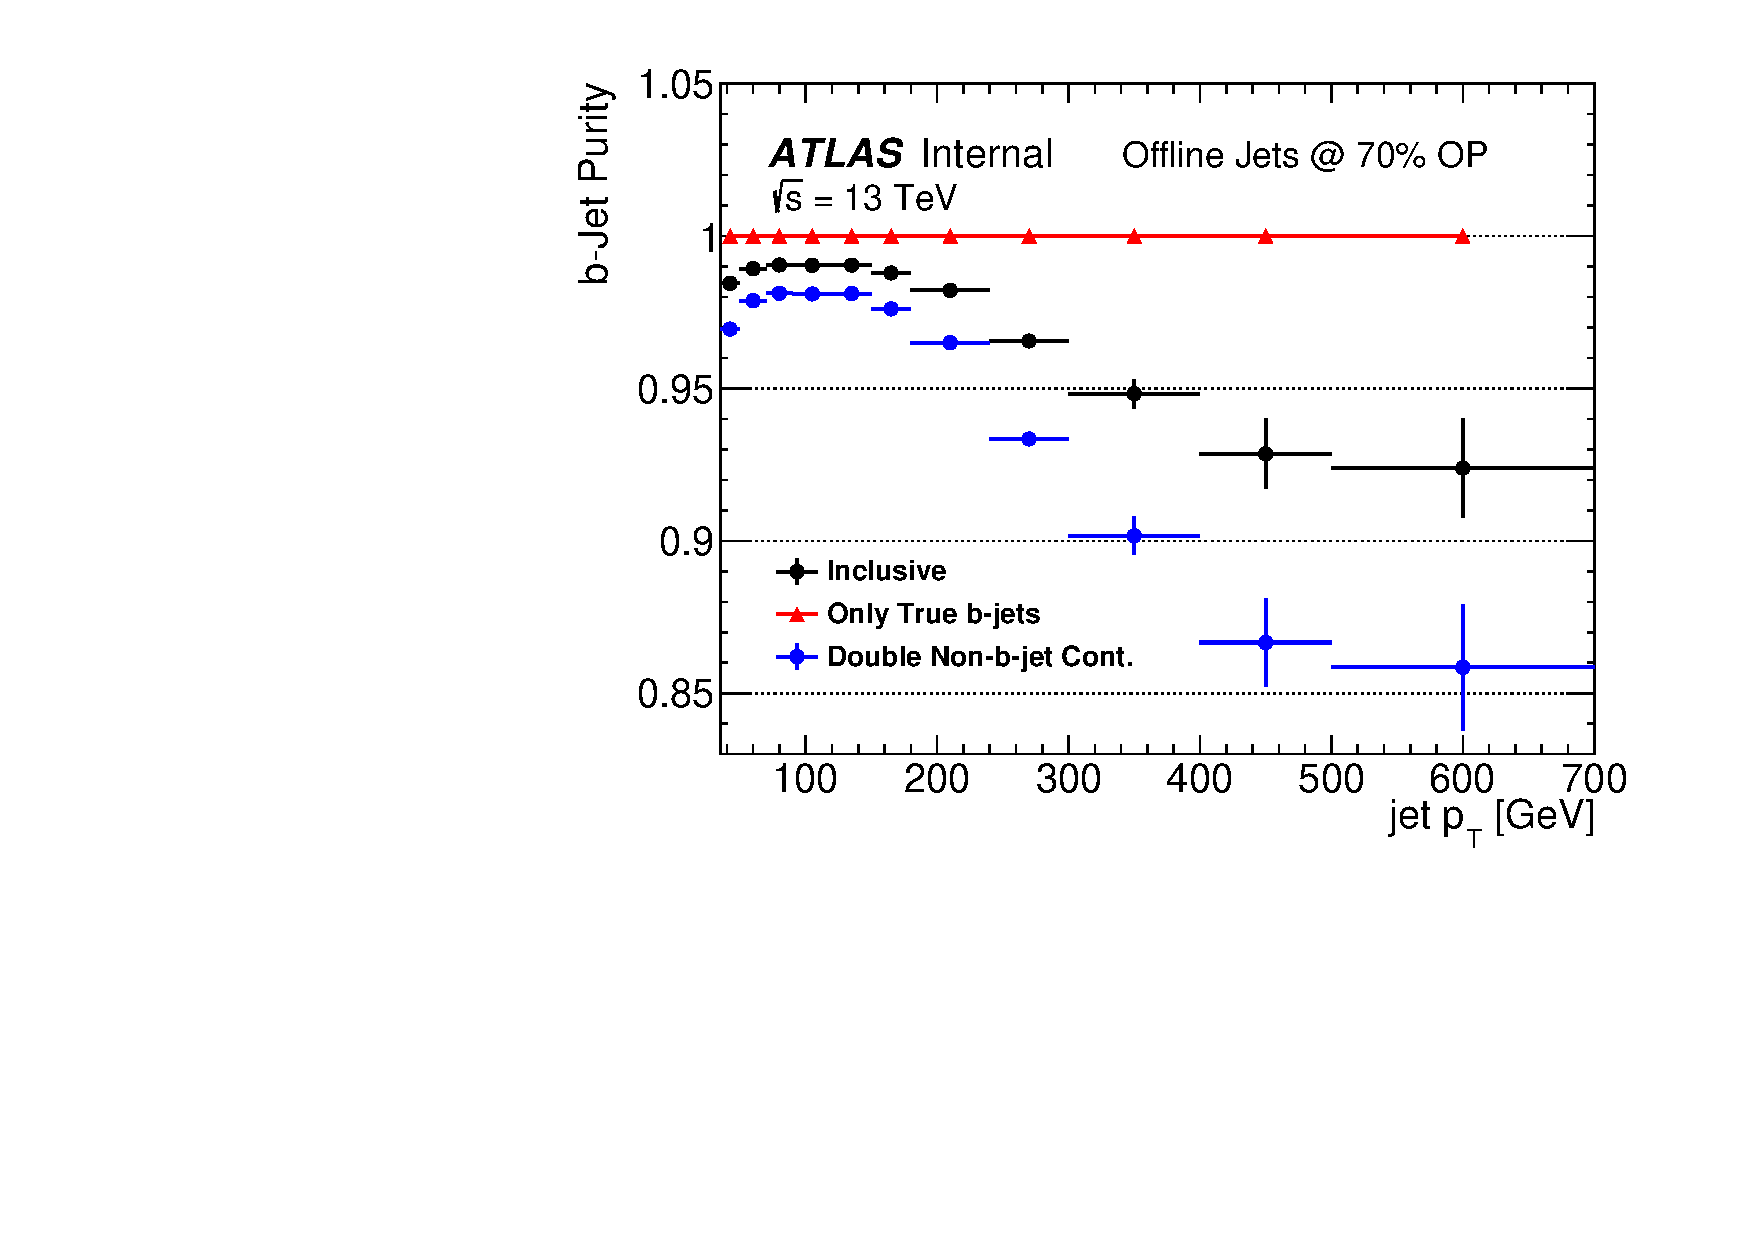
\includegraphics[width=0.47\linewidth, angle=0]{figs/Trigger/purityMC_variations.pdf}}
    \subcaptionbox{$b$-jet trigger efficiency}{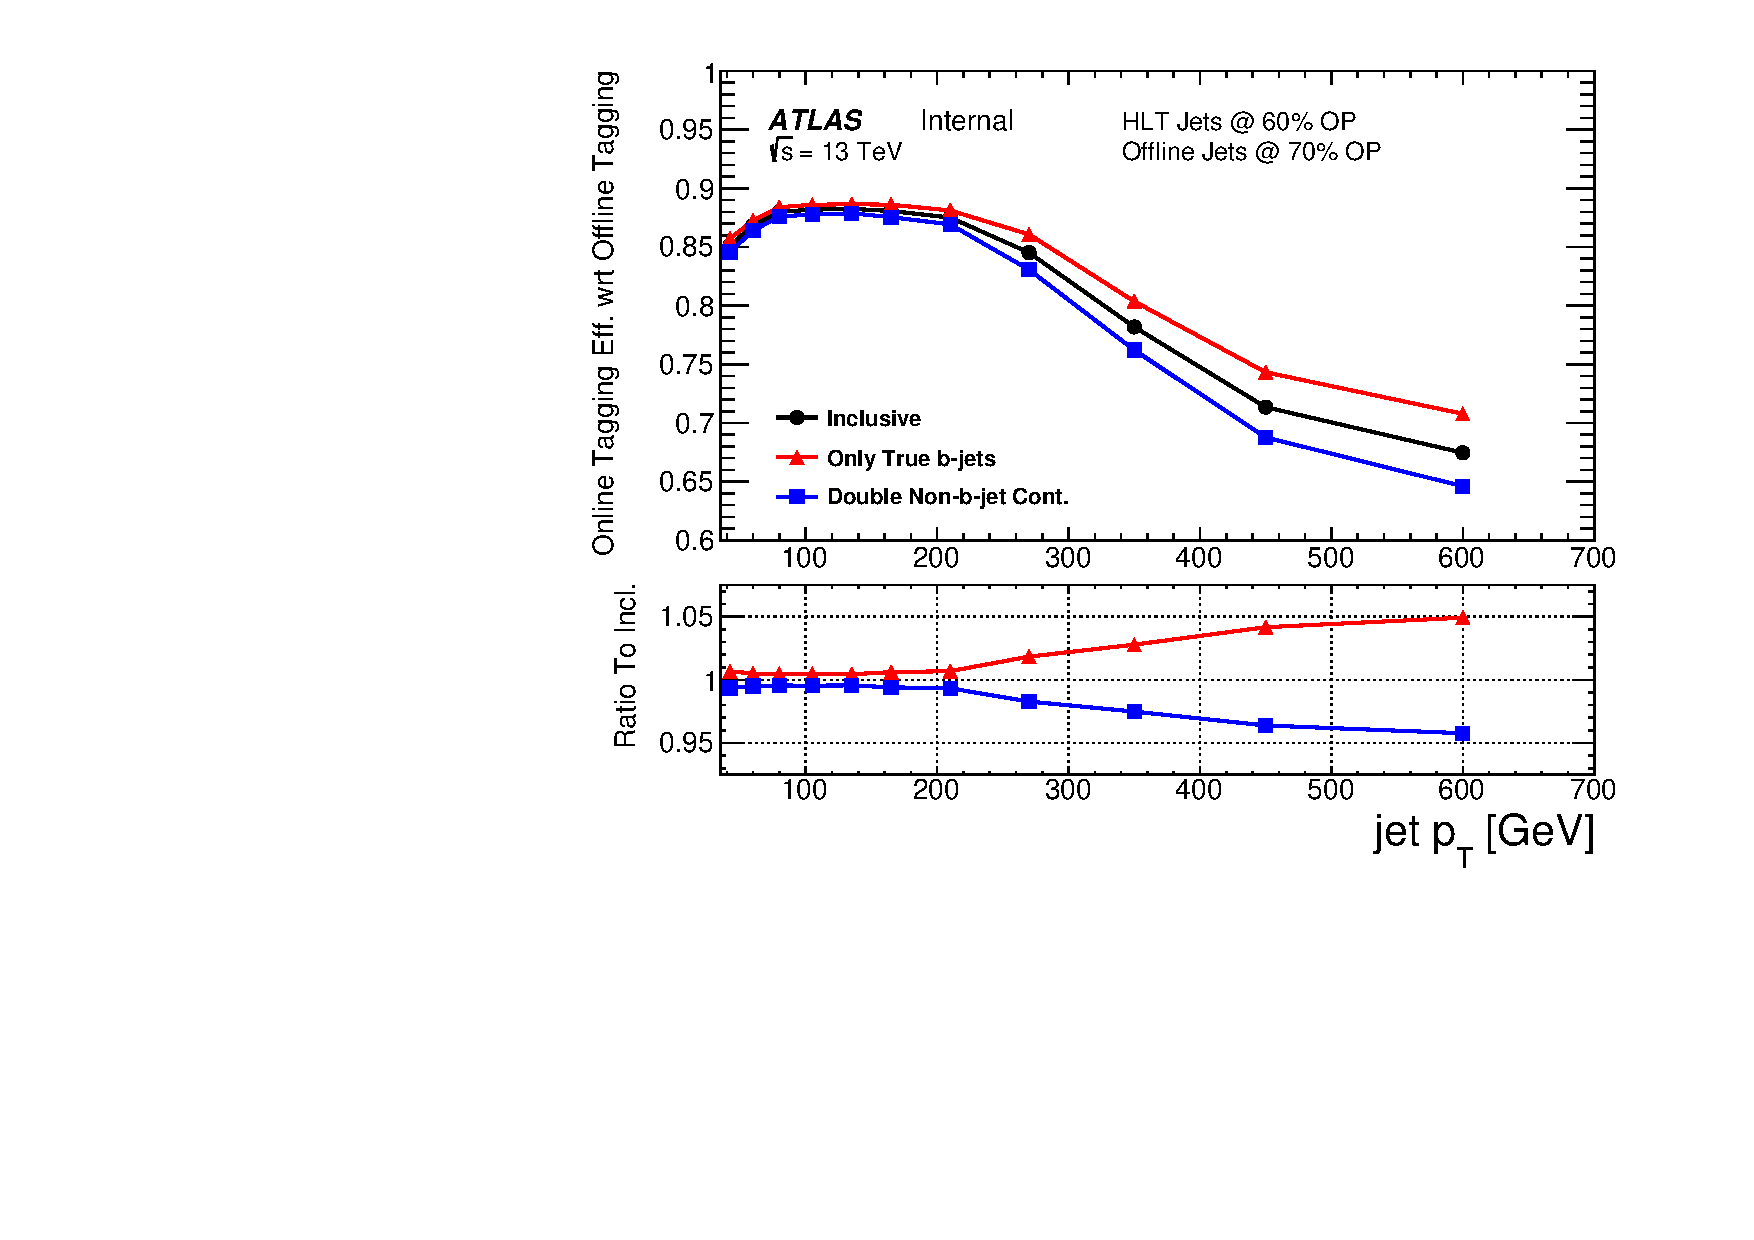
\includegraphics[width=0.47\linewidth, angle=0]{figs/Trigger/effMC_uncert_purity.pdf}}
  \end{center}
\vspace{-1em}
  \caption[The $b$-jet purity and $b$-jet trigger efficiency when the size of the non-$b$-jet contamination is systematically varied.]
          {\label{fig:Eff_Purity} Panel (a) shows the $b$-jet purity of the sample of inclusive jets (black) used in the $b$-jet trigger efficiency measurement
    and the $b$-jet purity in the systematic variations of true $b$-jets only (red) and when non-$b$-jet contamination is doubled (blue).
    Panel~(b) shows the 60\% operating point $b$-jet trigger efficiency with respect to an offline 70\% operating point for inclusive jets (black)
    and the systematic variations of true $b$-jets only (red) and double non-$b$-jet contamination (blue).
    The lower panel shows a ratio of the efficiencies in the systematic variations to the efficiency for inclusive jets.
    Statistical uncertainties are not shown in panel~(b).}
\end{figure}

Figure~\ref{fig:Eff_Purity}(b) shows the $b$-jet trigger efficiency for inclusive jets (black) and
for the systematic variations (red and blue),
the lower panel shows a ratio of the efficiencies for systematic variations to the efficiency for inclusive jets.
Statistical uncertainties are not shown in the figure, such that one can see distinguish between the systematic variations of the efficiency.
The ratio of efficiency for true $b$-jets to that of inclusive jets (red ratio line) is applied as a correction to the final efficiency measured in data
to account for the effect of non-$b$-jet contamination.
The bin-by-bin maximum fractional difference in efficiency due to systematic variations (red or blue ratio line) is taken as symmetric uncertainty.


\noindent
\textbf{(2)~~Non-$b$-jet efficiency uncertainty}
\label{sec:trig-lightTrigEff}

The efficiency of the $b$-jet trigger for non-$b$-jets is not measured and could be mismodelled in simulation.
To derive a non-$b$-jet efficiency systematic uncertainty; up and down systematic variations are created by doubling and halving the non-$b$-jet efficiency respectively.
For the up variation the non-$b$-jet efficiency is limited to be no greater than the efficiency of true $b$-jets, which avoids unrealistic results.
To illustrate the systematic variations,
Figure~\ref{fig:Eff_LTrigEff}(a) shows the $b$-jet trigger efficiency in simulation for non-$b$-jets in the nominal case and in the two systematic variations considered.

Figure~\ref{fig:Eff_LTrigEff}(b) shows the $b$-jet trigger efficiency in simulation for inclusive jets in the nominal case and for the two systematic variations.
Statistical uncertainties are not shown in the figure, such that one can see distinguish between the systematic variations of the efficiency.
The maximum fractional bin-by-bin difference in efficiency for inclusive jets between the nominal and the systematic variations,
as shown in the ratio plot of Figure~\ref{fig:Eff_LTrigEff}(b),
is taken as a symmetric uncertainty.

\begin{figure}[!ht]
  \begin{center}
    \captionsetup[subfigure]{aboveskip=0pt,justification=centering}
    \subcaptionbox{Non-$b$-jets}{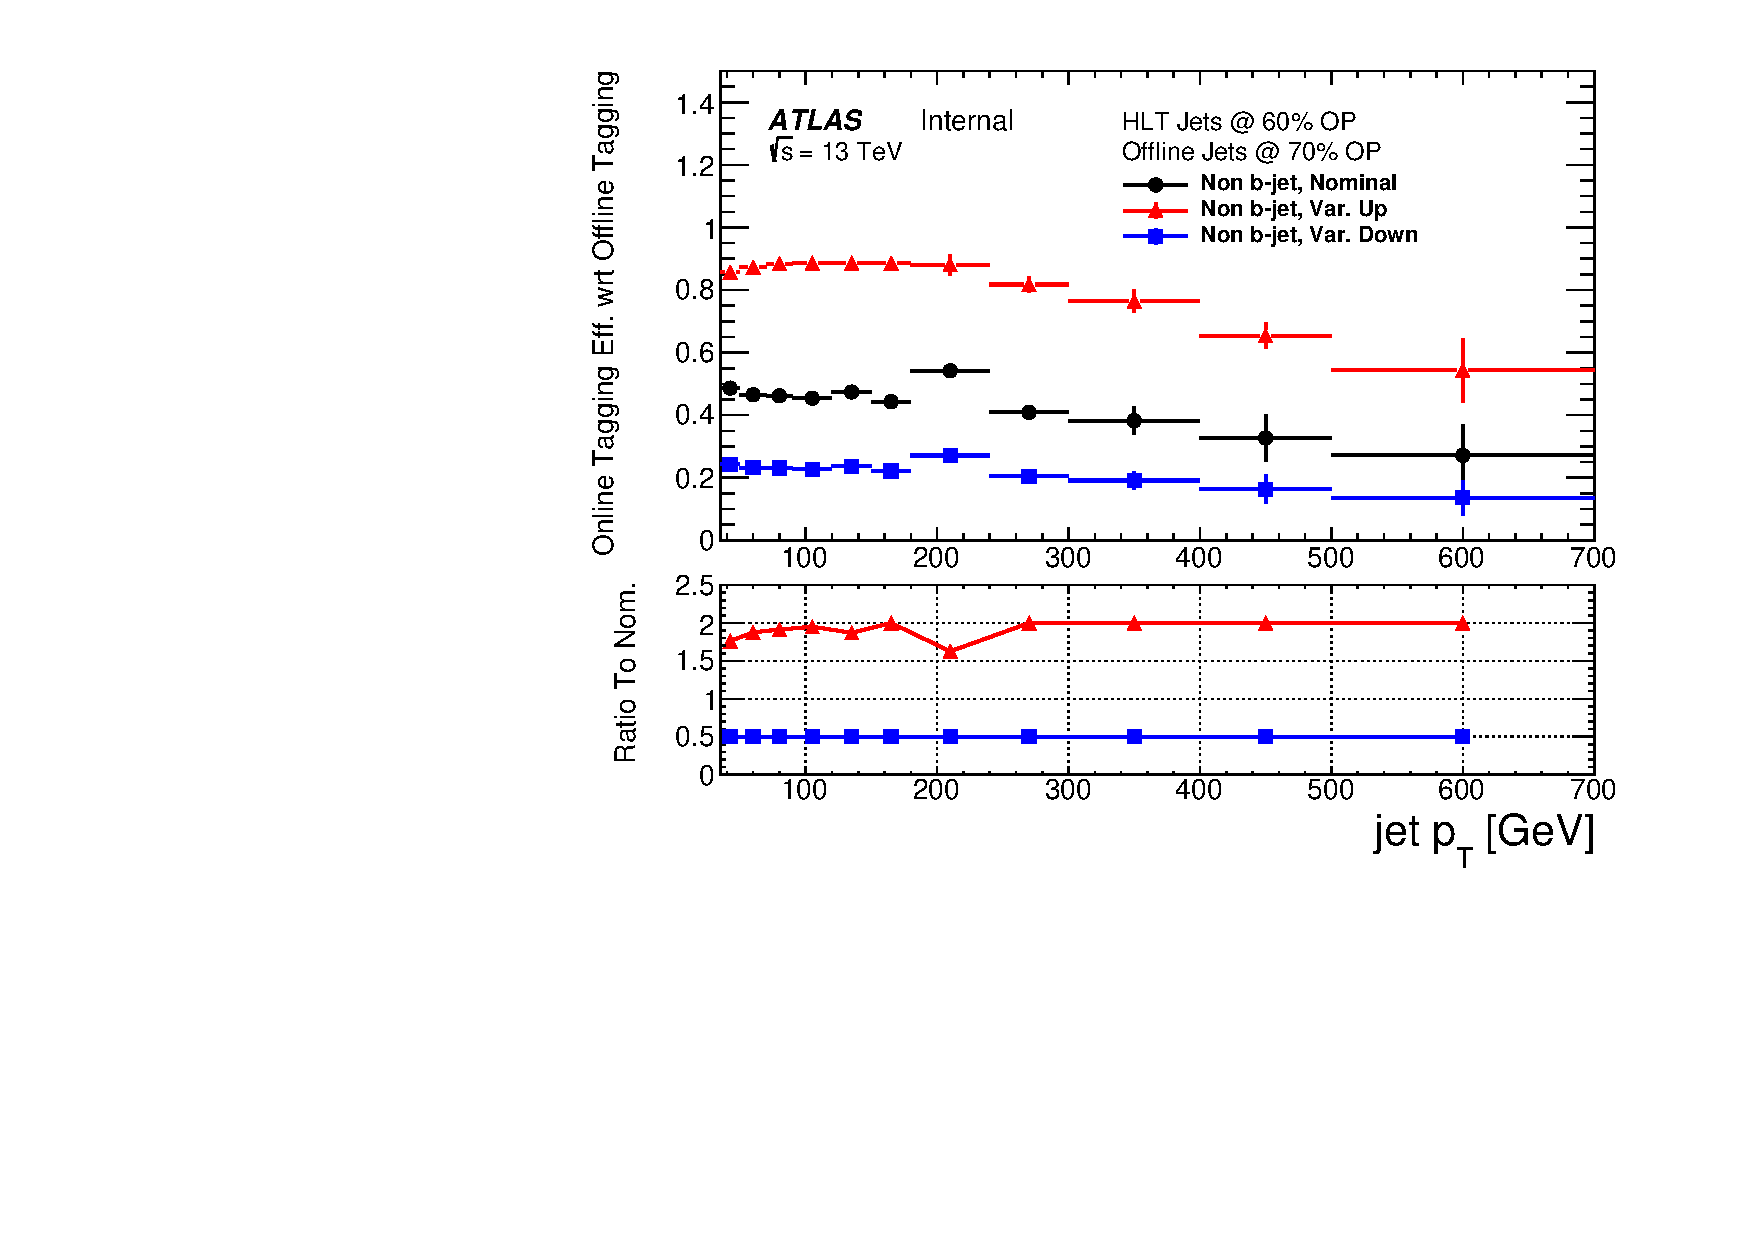
\includegraphics[width=0.47\linewidth, angle=0]{figs/Trigger/effMC_variations_LTrigEff.pdf}}
    \subcaptionbox{Inclusive jets}{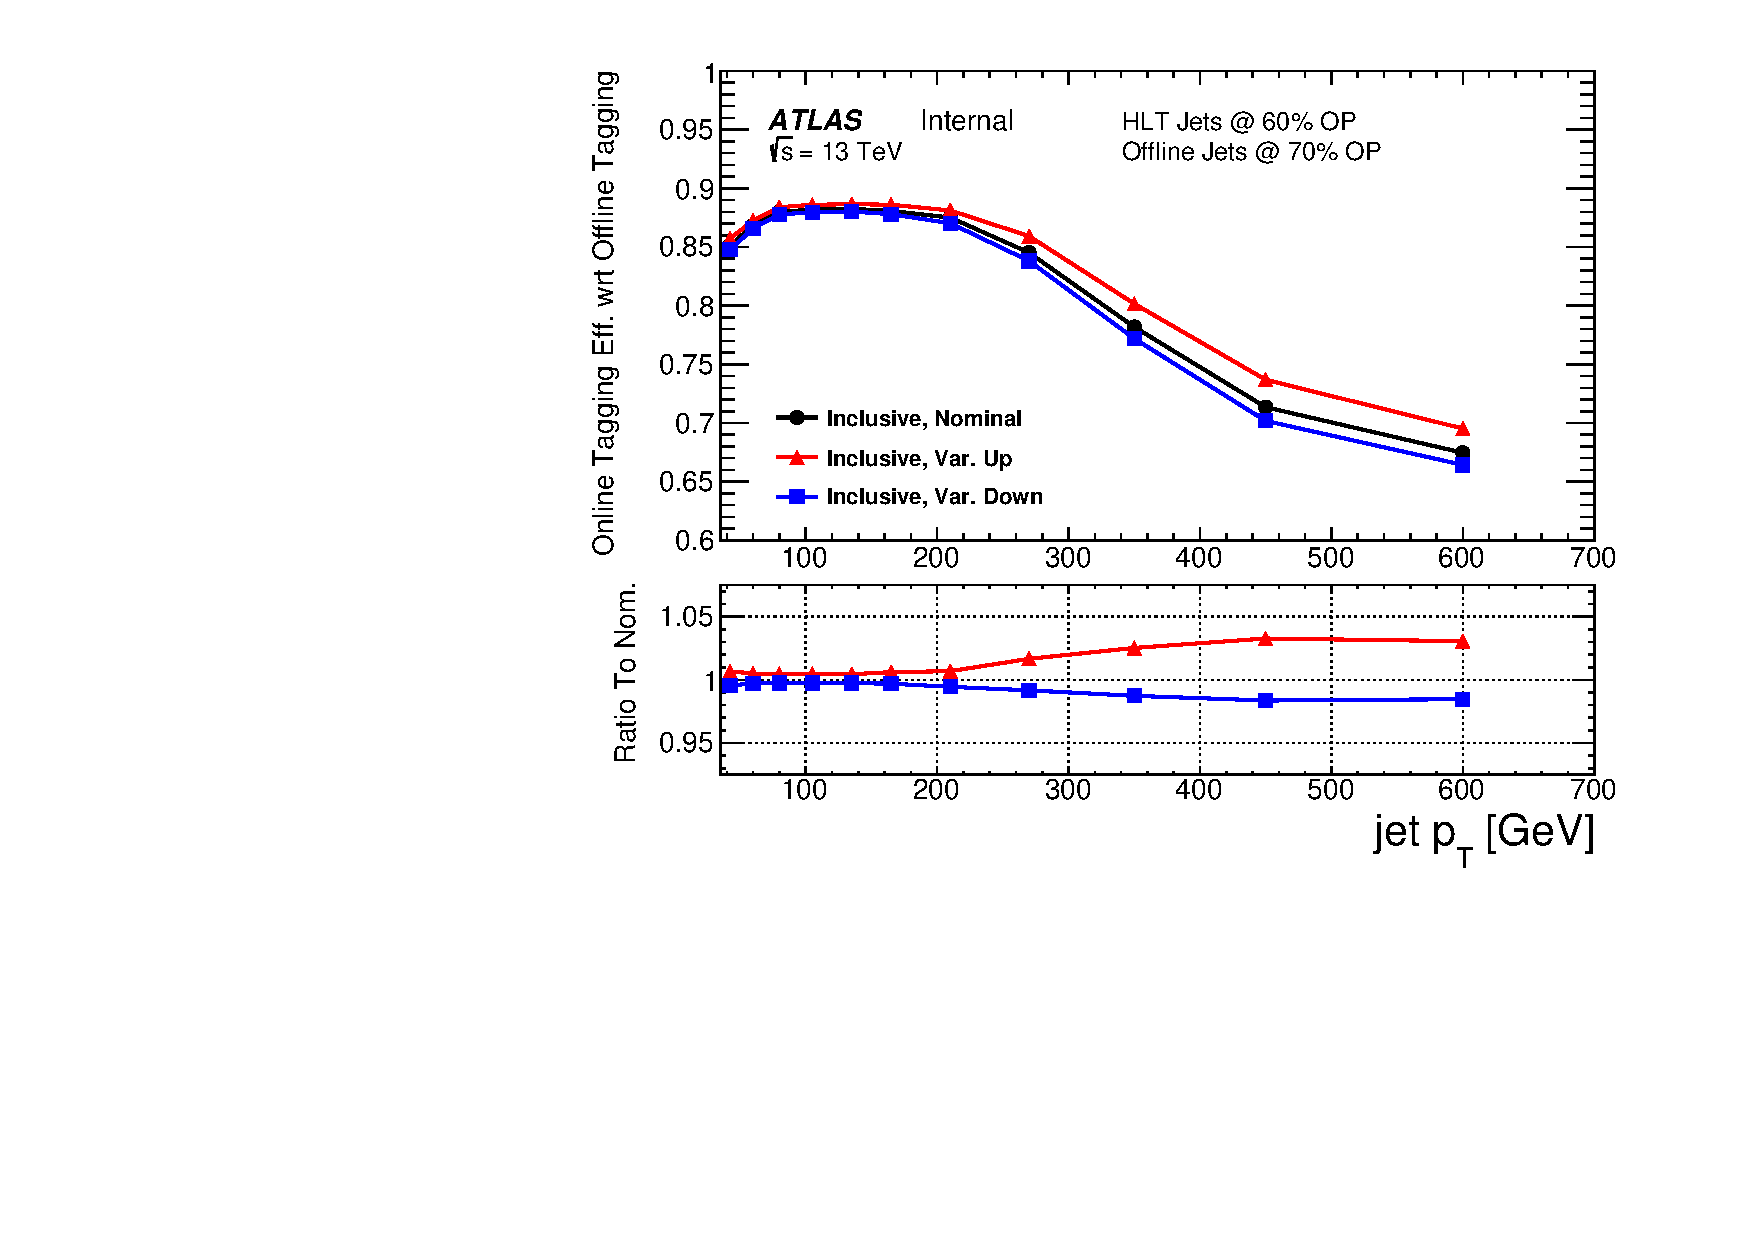
\includegraphics[width=0.47\linewidth, angle=0]{figs/Trigger/effMC_uncert_LTrigEff.pdf}}
  \end{center}
\vspace{-1em}
  \caption[The $b$-jet trigger efficiency for  non-$b$-jets and inclusive jets for systematic variations of the non-$b$-jet efficiency.]
          {The 60\% operating point $b$-jet trigger efficiency with respect to the offline 70\% operating point
            for (a) non-$b$-jets and (b) inclusive jets in simulated events
            for the  nominal case (black) and the systematic variations where the non-$b$-jet efficiency has been halved (blue) and doubled (red).
            The lower panel in both plots show the ratio of the efficiency of the systematic variation efficiency to the nominal inclusive efficiency.
            Statistical uncertainties are not shown in panel~(b).
  }
  \label{fig:Eff_LTrigEff}
\end{figure}

%\begin{figure}[!ht]
%  \begin{center}
%    \captionsetup[subfigure]{aboveskip=0pt,justification=centering}
%    \subcaptionbox{}{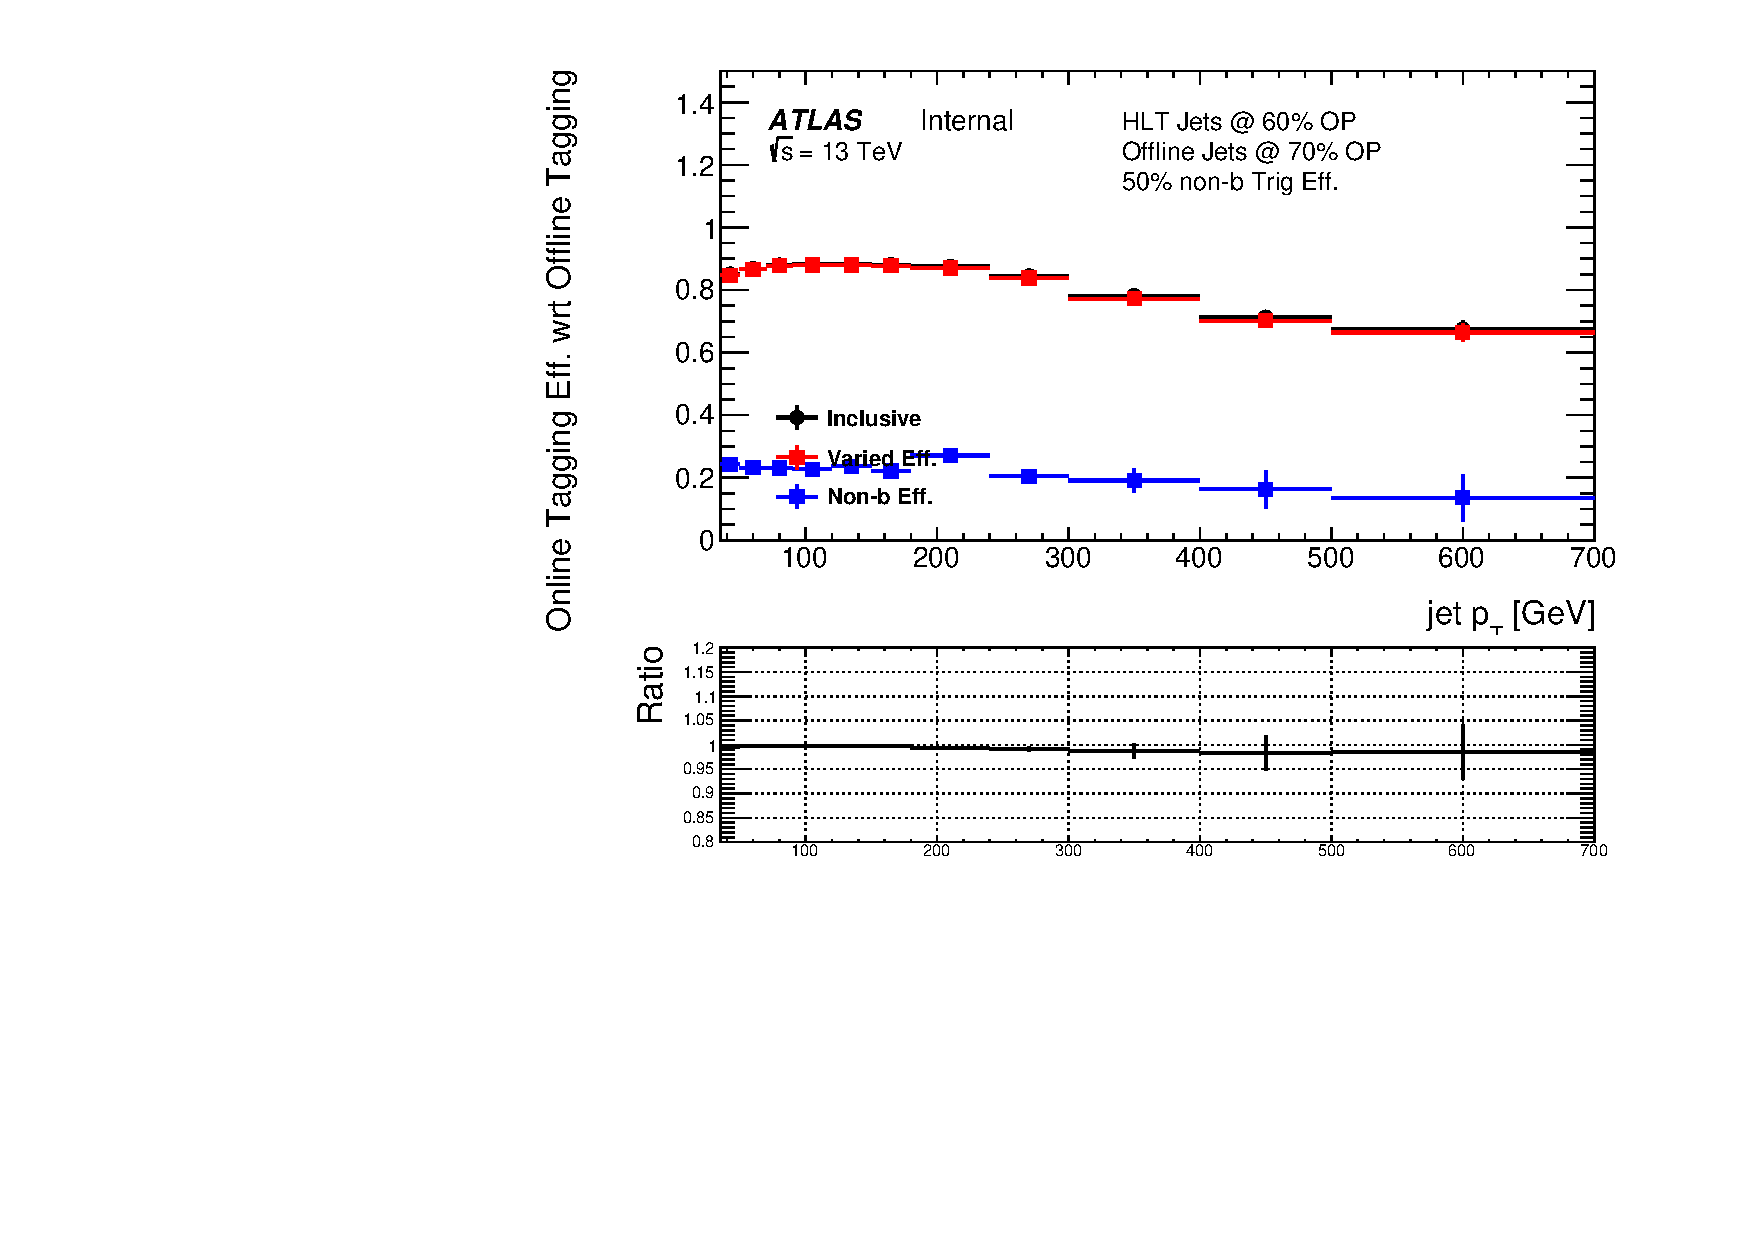
\includegraphics[width=0.47\linewidth, angle=0]{figs/Trigger/effMC_jetPt_lowLTrigEff.pdf}}
%    \subcaptionbox{}{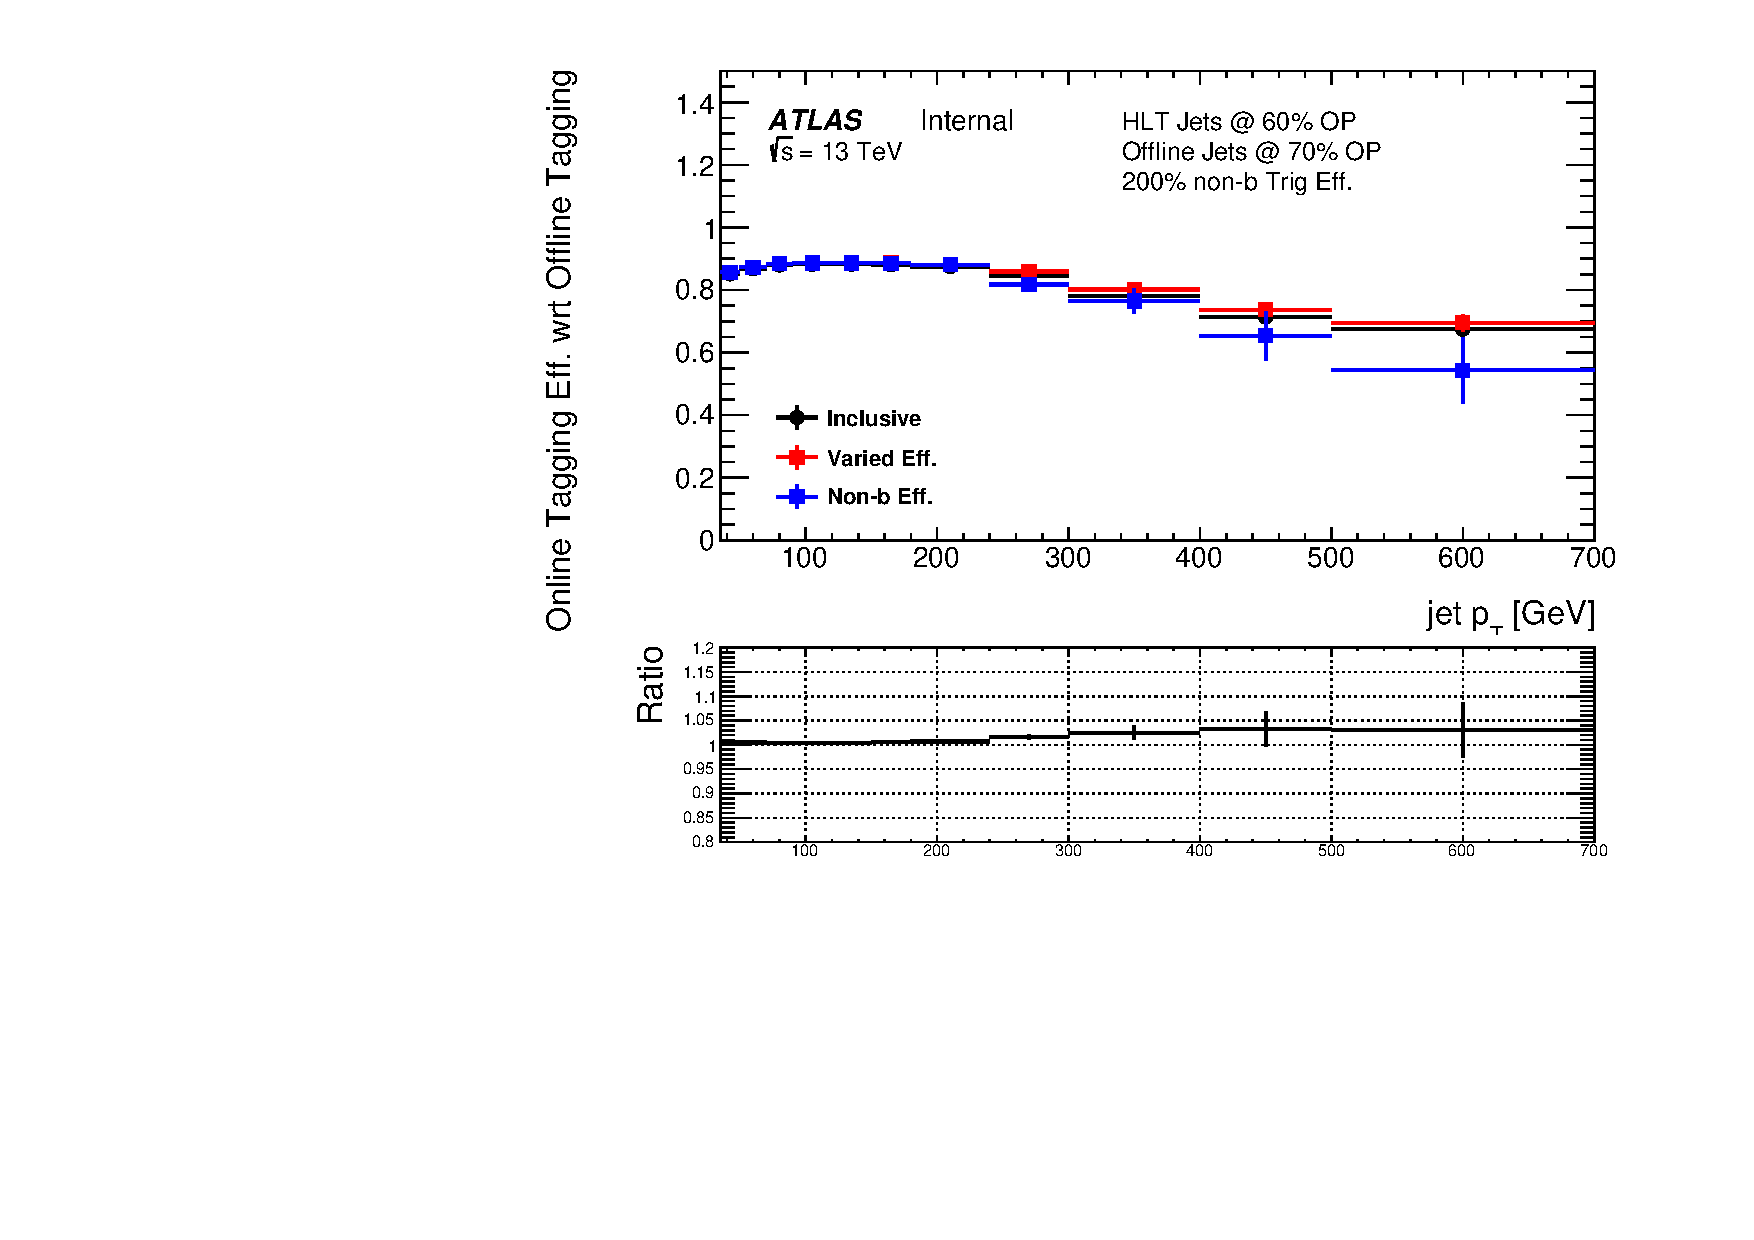
\includegraphics[width=0.47\linewidth, angle=0]{figs/Trigger/effMC_jetPt_upLTrigEff.pdf}}
%  \end{center}
%  \caption{The 60\% operating point $b$-jet trigger efficiency with respect to the offline 70\% operating point
%    for nominal inclusive case (black) compared to varied inclusive case (red) and just non $b$-jets (blue)
%    in the case where non $b$-jet efficiency has been halved (a) and doubled (b) for a simulated $t\bar{t}$ sample.
%    The lower panel in both plots show the ratio of the varied inclusive efficiency to the nominal inclusive efficiency.
%  }
%  \label{fig:Eff_LTrigEff}
%\end{figure}

\FloatBarrier

\newpage
\noindent
\textbf{(3)~~High-\pT{}~extrapolation}
\label{sec:trig-highPtExtrap}

%The $b$-jet trigger efficiency measurement in data is limited for high-\pT~jets due to reduced statistics in data.
There is a limited number of high-\pT{} inclusive jets in the data-set which
causes large statistical fluctuations in the $b$-jet trigger efficiency in data, as shown in Figure~\ref{fig:Full_bslt2mm_eff}(a).
Therefore, the $b$-jet trigger efficiency shape from simulation is used to extrapolate the efficiency for jet-\pT{} $>$ 240 GeV.
$\,$This $p_T$ range is chosen for extrapolation as in this region the data statistical uncertainty is the dominant uncertainty.

The extrapolation procedure uses three fits to produce a ``corrected simulation'' $b$-jet trigger efficiency.
The three fits are:
\vspace{-0.5em}
\begin{itemize}[leftmargin=*]  
  \setlength\itemsep{0.5em}
\item \textbf{Normalisation Fit}: A \textit{`normalised simulation'} efficiency is created by applying
  a normalisation factor derived by performing a single-constant fit
  to the ratio of the $b$-jet trigger efficiency in data and simulation.
  The lowest \pT{} bin has an inconsistent data/simulation ratio compared to other low-\pT{} bins, so is excluded from the fit
  \footnote{\ The discrepancy is shown below in Table~\ref{tab:bTrig_jetSys}. The difference is within purity uncertainties.}.
  The normalisation fit is shown in Figure~\ref{fig:bTrig_mcExtrap}(a),
  the uncertainty on the fit-parameter is used as a systematic uncertainty.
  
\item \textbf{Linear Correction Fit}:
  A \textit{`corrected simulation'} efficiency is created by applying a linear correction factor to the normalised simulation efficiency.
  The correction is derived by performing a linear fit to the ratio of the $b$-jet trigger efficiency in data and the normalised simulation
  in the range jet-\pT{} $>$ 240 GeV, as shown in Figure~\ref{fig:bTrig_mcExtrap}(b).
  To estimate an uncertainty on the linear correction the gradient of the fit is varied within uncertainties
  whilst the point at which the fit crosses 1 is kept constant.
  The maximum difference between the nominal fit and the systematic variations is used as a symmetric uncertainty.
  Figure~\ref{fig:bTrig_mcExtrap}(c) shows the $b$-jet trigger efficiency in data compared to the corrected simulation,
  in the lower panel the blue lines represent the linear correction uncertainties.
  
\item \textbf{Quadratic Systematic Fit}: 
  To estimate an uncertainty on the choice of the linear functional form as the correction factor,
  a quadratic function is used to fit the data and corrected simulation ratio
  as shown in Figure~\ref{fig:bTrig_mcExtrap}(d).
  The difference of the quadratic fit from one is considered as the functional form systematic uncertainty.
\end{itemize}

For jet-\pT{} $>$ 240 GeV the $b$-jet trigger efficiency in data and thus the numerator of the data/simulation scale factors is given by the corrected simulation.
The systematic uncertainty on the extrapolation is defined as the uncertainty from the normalisation fit
added to the bin-by-bin maximum of the uncertainty from the linear correction fit and the uncertainty from the quadratic systematic fit.
%The quadratic and linear uncertainties are not combined;
%as if the result from the quadratic fit result lies within the linear uncertainty then it is deemed that functional choice was adequete for that bin.
The uncertainties on the high-\pT~extrapolation procedure  are summarised in Table~\ref{tab:bTrig_extrapSyst}.

\begin{figure}[!ht]
\begin{center}
\captionsetup[subfigure]{aboveskip=0pt,justification=centering}
  \subcaptionbox{Normalisation fit} {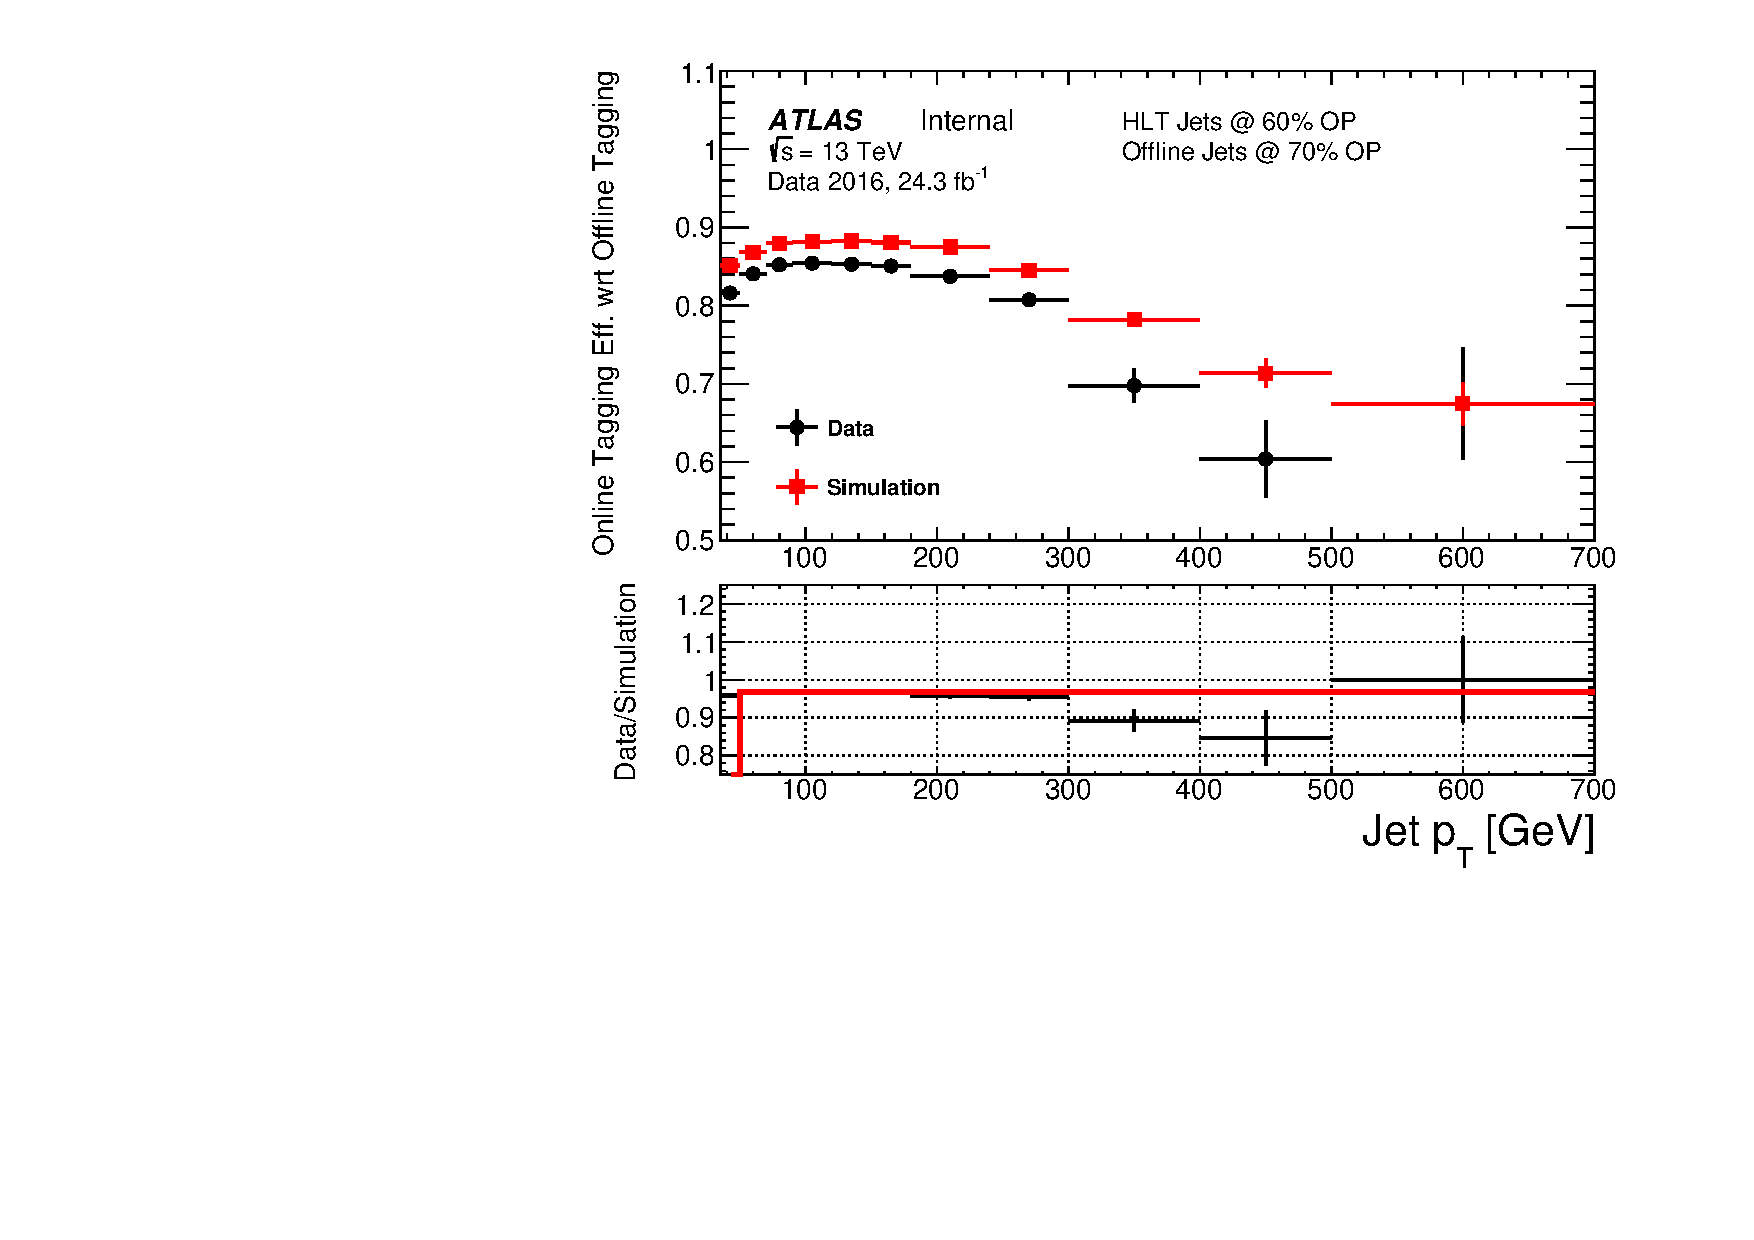
\includegraphics[width=0.47\linewidth, angle=0]{figs/Trigger/Full_GRL_bslt2mm_effFit_jetPt.pdf} }
  \subcaptionbox{Linear correction fit} {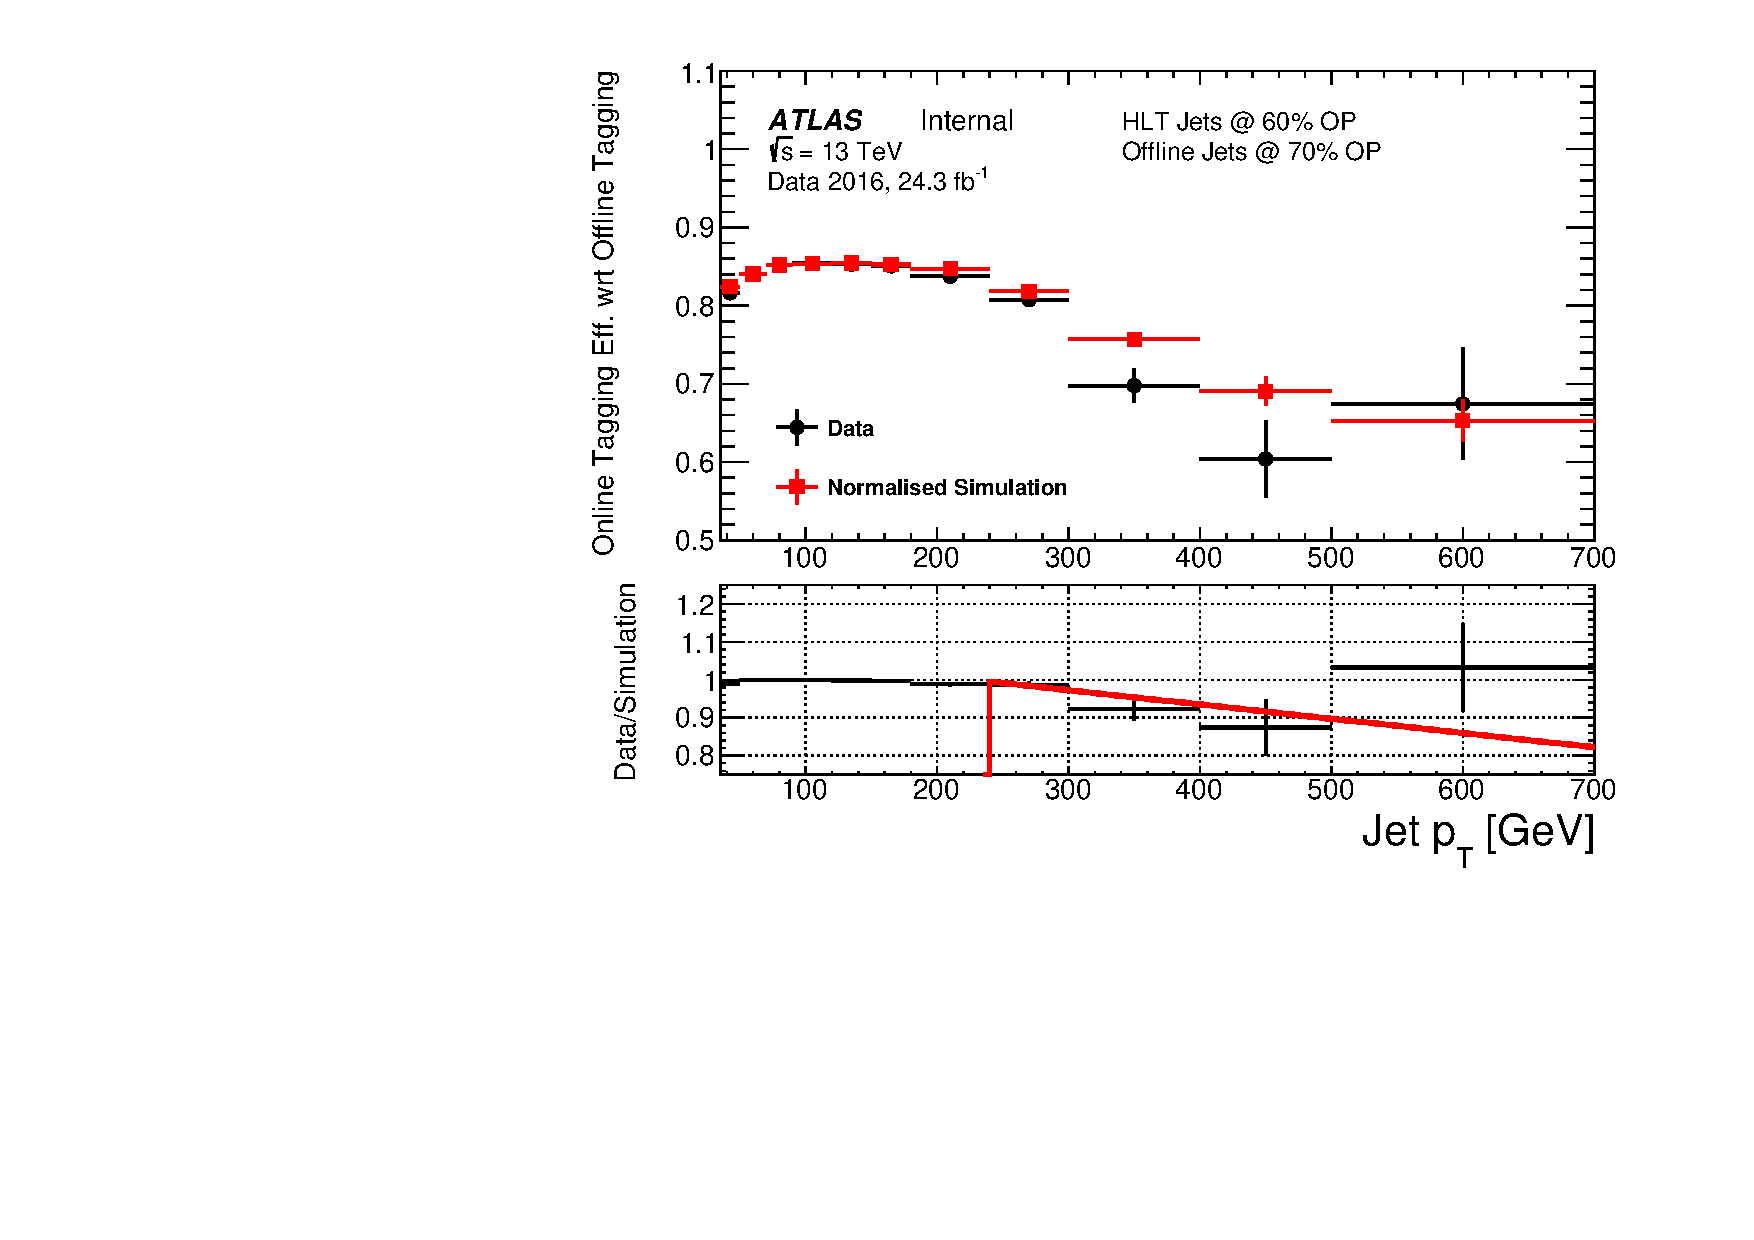
\includegraphics[width=0.47\linewidth, angle=0]{figs/Trigger/Full_GRL_bslt2mm_effNormFit_jetPt.pdf}} \\
  \subcaptionbox{Linear correction uncertainties} {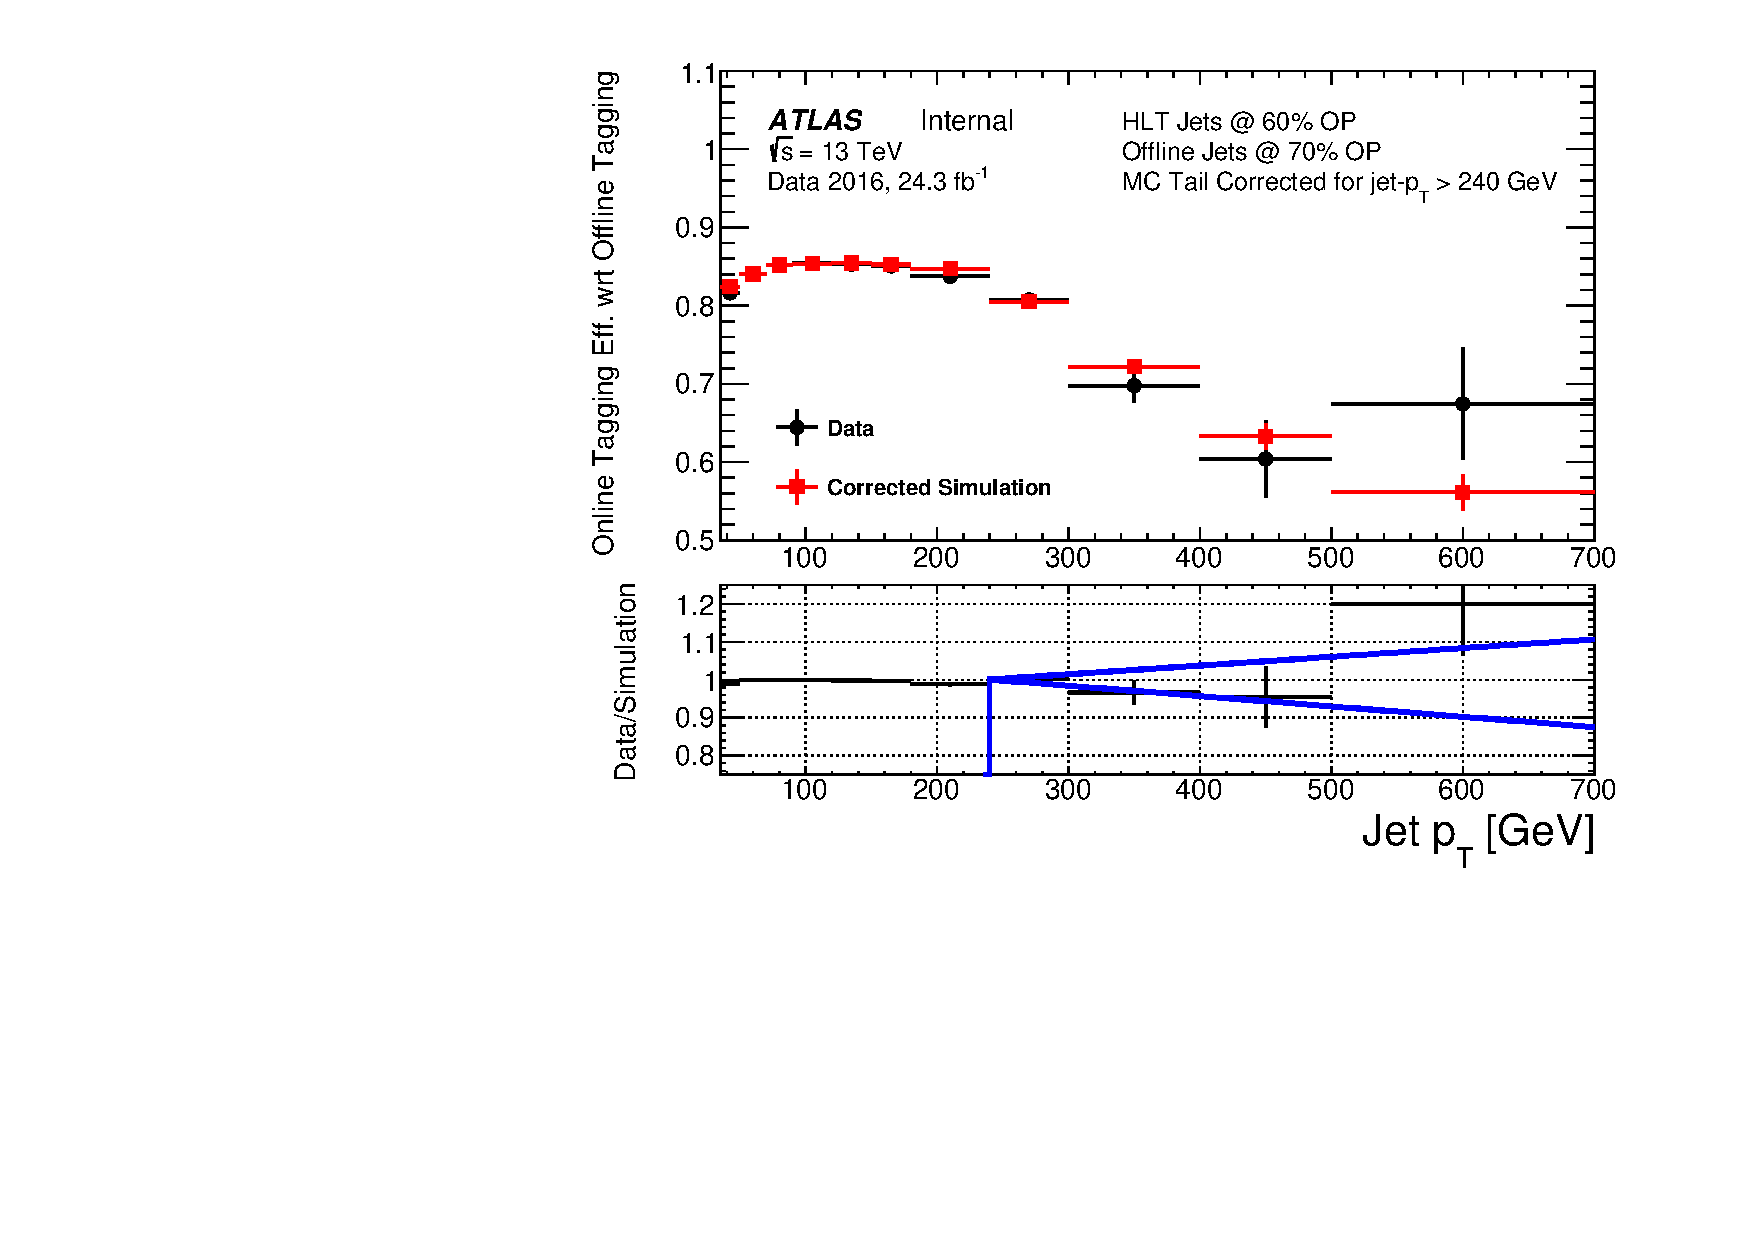
\includegraphics[width=0.47\linewidth, angle=0]{figs/Trigger/Full_GRL_bslt2mm_effCorrShapeErr_jetPt.pdf}}
  \subcaptionbox{Quadratic fit } {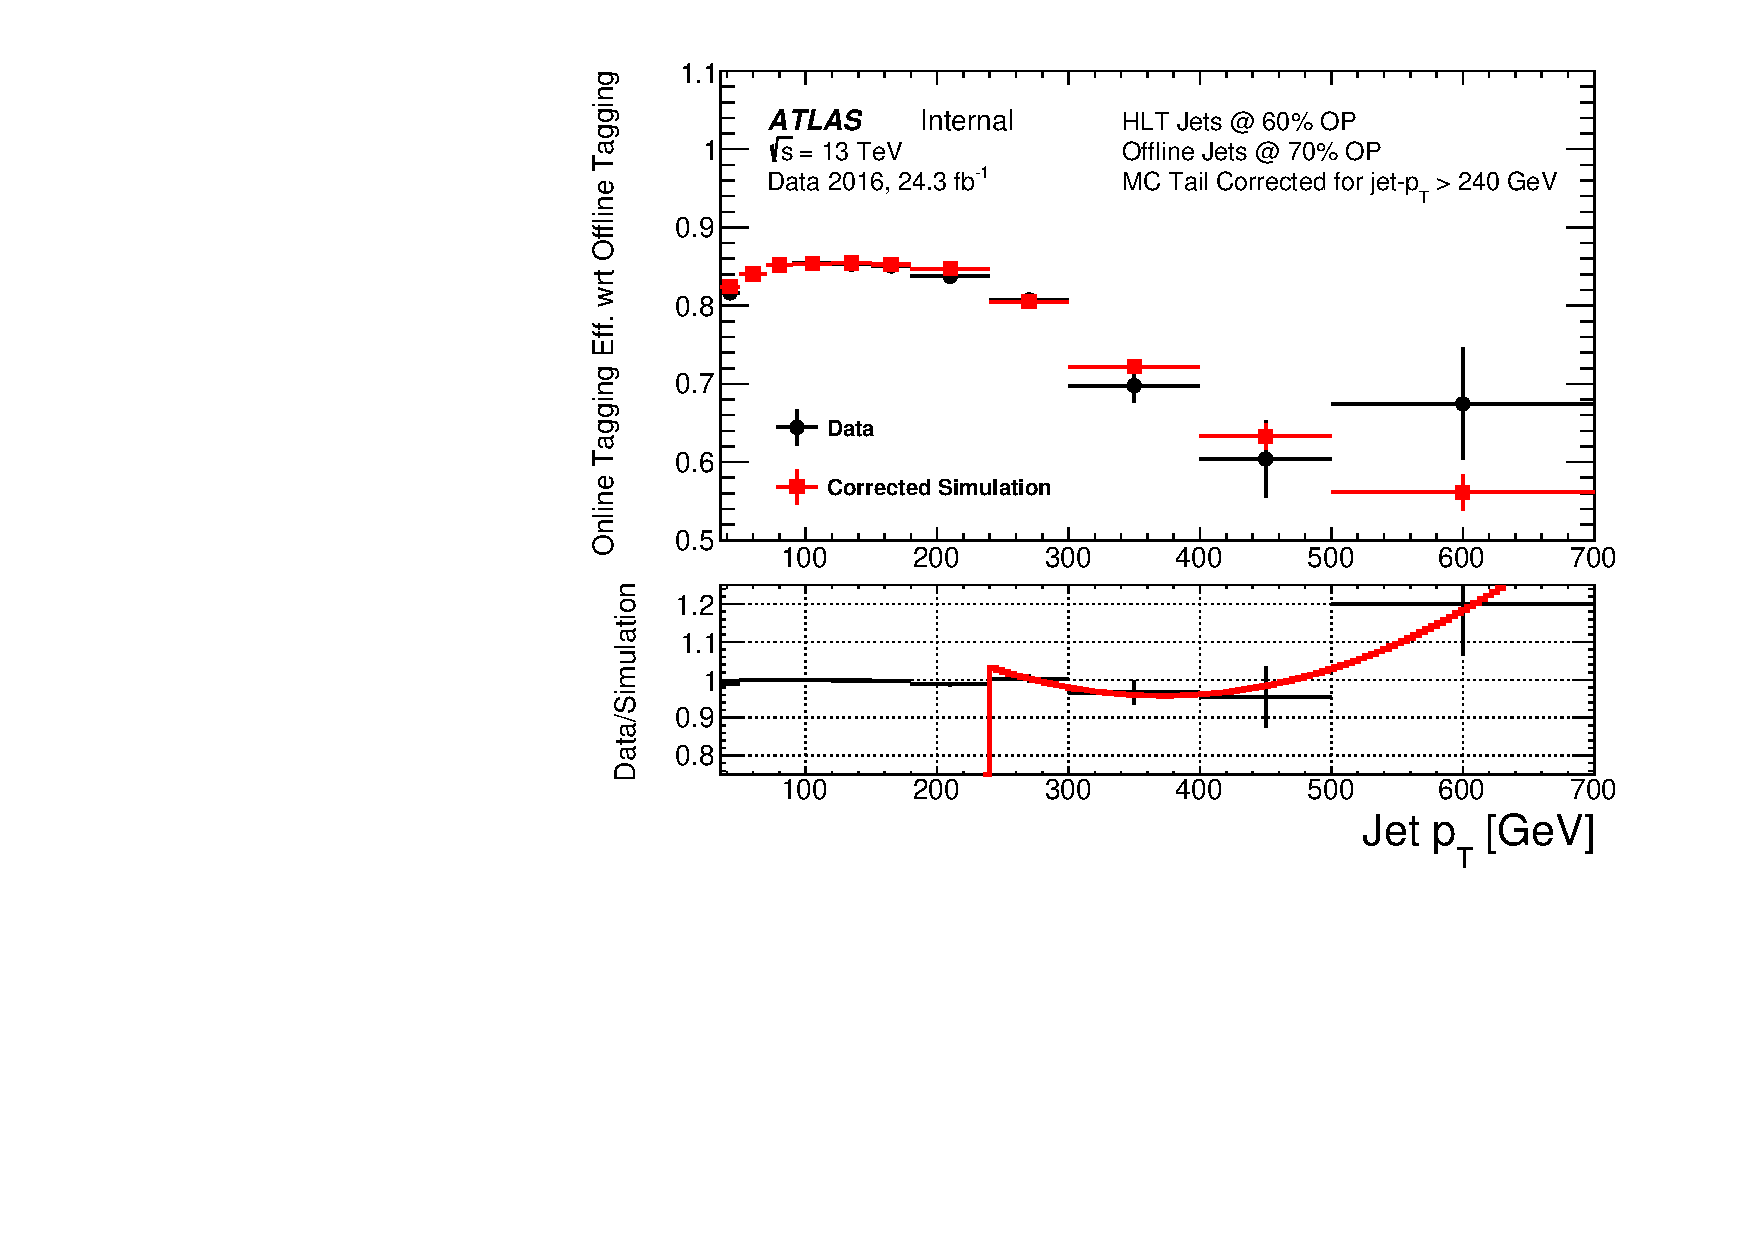
\includegraphics[width=0.47\linewidth, angle=0]{figs/Trigger/Full_GRL_bslt2mm_effCorrFitQuad_jetPt.pdf}}
  %\subcaptionbox{Extrapolation closure}{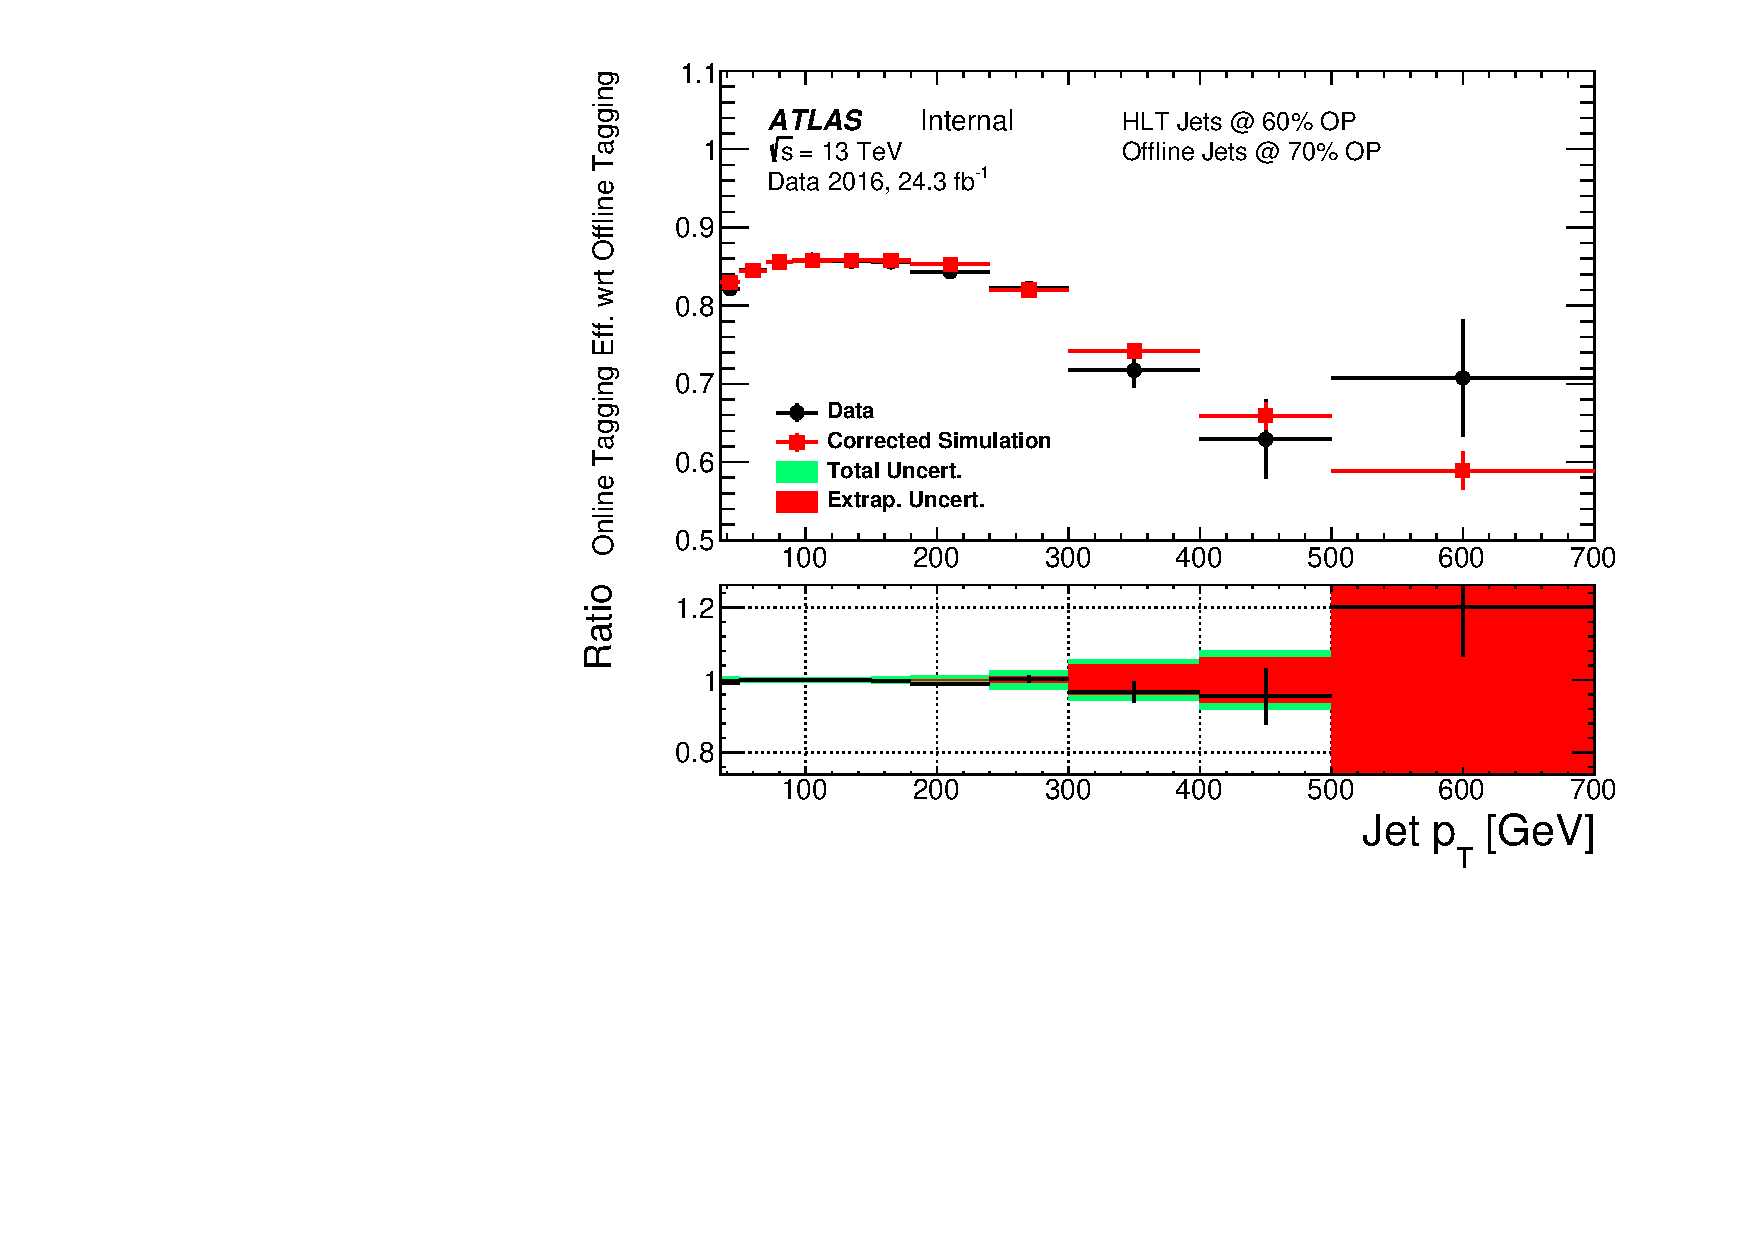
\includegraphics[width=0.47\linewidth, angle=0]{figs/Trigger/fullSys_EfficiencyComp_jetPt.pdf}}
\end{center}
\vspace{-0.8em}
\caption[A figure to demonstrate the stages of the high-\pT~extrapolation procedure for the $b$-jet trigger efficiency measurement.]
        {A figure to demonstrate the stages of the high-\pT~extrapolation procedure for the 60\% operating point $b$-jet trigger efficiency with respect to the offline 70\% operating point.
          The $b$-jet trigger efficiency as a function of jet-\pT{} is shown for data (black) and simulation after corrections have been applied (red);
          the corrections used are labelled and are described in the text.
          Panel (a) shows the normalisation fit,
          panel (b) shows the linear correction fit,
          panel (c) shows linear correction uncertainties (blue lines) and
          panel (d) shows the quadratic fit.
          %Panel (e) compares data and corrected simulation with the high-\pT{} extroplation uncertainties (red area) and total uncertainties (green area) shown in the ratio.
        }
        \label{fig:bTrig_mcExtrap}
\end{figure}

\vspace{0.5em}
\begin{table}[!ht]
  \begin{center}
\begin{tabular}{|c||c||c|c|c|c|}
  \hline
  Jet pT [GeV] & MC Extrap. & Normalisation & Linear Fit  & Quadratic Fit \\
  \hline
  240-300 &  0.8\% & 0.0\% & 0.8\% &  0.3\% \\
  300-400 &  4.0\% & 0.0\% & 2.9\% &  4.0\% \\
  400-500 &  5.6\% & 0.0\% & 5.6\% &  1.7\% \\
  500-700 & 18.0\% & 0.0\% & 9.6\% & 18.0\% \\
  \hline
\end{tabular}
%  \vspace{}
\caption{A table showing the systematic uncertainty assigned for the high-\pT~extrapolation.}
\label{tab:bTrig_extrapSyst}
\vspace{-1em}
  \end{center}
\end{table}


As a closure test of the high-\pT~extrapolation procedure,
Figure~\ref{fig:bTrig_jetSys_effComp} shows the $b$-jet trigger efficiency in data and corrected simulation,
the lower panel shows the ratio with extrapolation and total uncertainties overlaid.
For jet-\pT{} $>$ 240 GeV, the data and corrected simulation are consistent within the extrapolation uncertainties.

\begin{figure}[!ht]
\begin{center}
    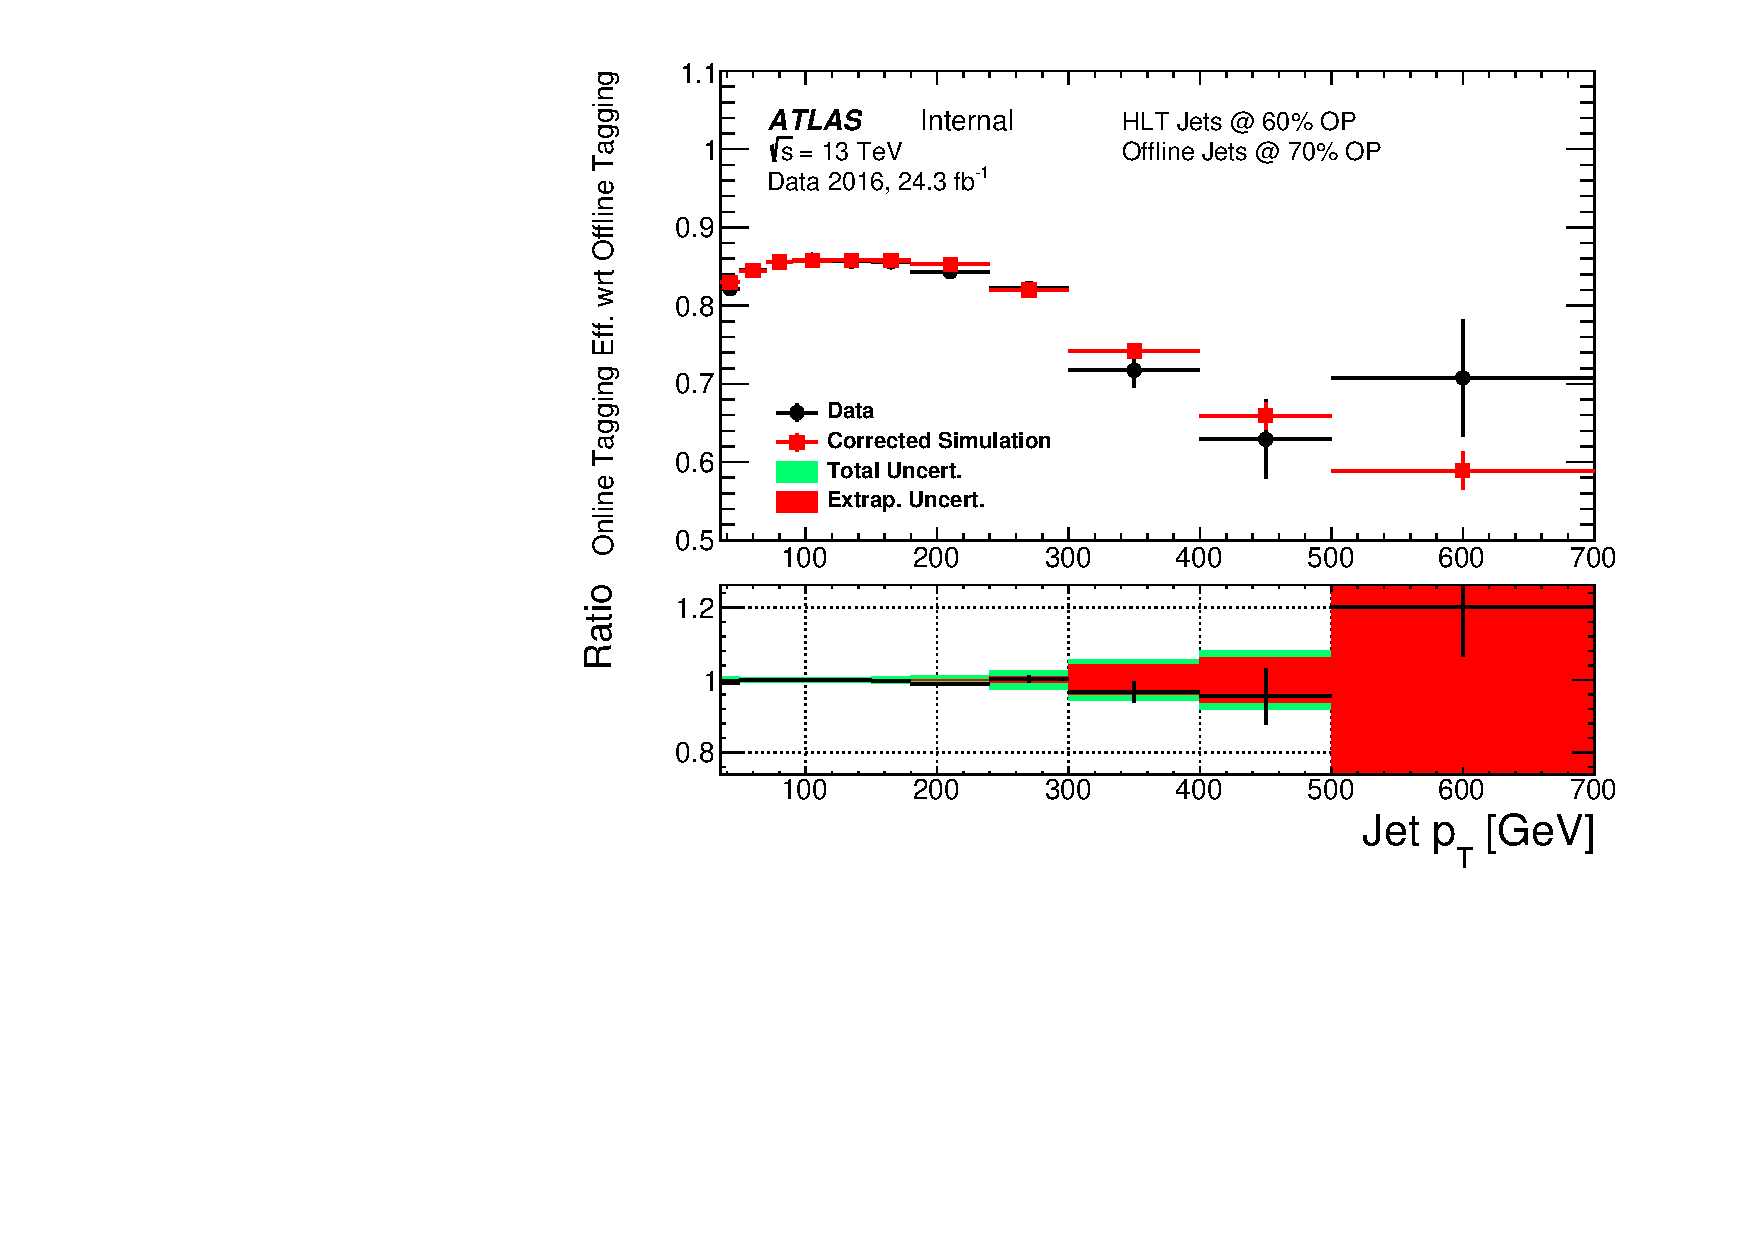
\includegraphics[width=0.5\linewidth, angle=0]{figs/Trigger/fullSys_EfficiencyComp_jetPt.pdf}
  \end{center}
\vspace{-1em}
\caption[The $b$-jet trigger efficiency measured in data and the corrected simulation as a function of offline jet-\pT.
  The extrapolation uncertainties and total uncertainty are shown.
    \label{fig:bTrig_jetSys_effComp}]
        {
    The 60\% operating point $b$-jet trigger efficiency with respect to the offline 70\% operating point
    as measured in data (black) and the corrected simulation (red) as a function of offline jet-\pT.
    In the ratio plot in the lower panel the extrapolation uncertainties (red band) and total uncertainty (green band) are overlaid.
    \label{fig:bTrig_jetSys_effComp}
  }
\end{figure}

\newpage

The raw measurements of the $b$-jet trigger efficiency from Figure~\ref{fig:Full_bslt2mm_eff}
and the additional corrections and systematic uncertainties described above can be brought together.
In Figure~\ref{fig:Full_bslt2mm_eff}(b) it is shown that, whilst efficiency does depend on jet-$\eta$,
the data to simulation ratio is flat with respect to jet-$\eta$.
Therefore the $b$-jet trigger efficiency and data/simulation scale factors are derived as a function of jet-\pT{} only. 
The jet-level $b$-jet trigger efficiency measurement is shown in Figure~\ref{fig:bTrig_jetSys}(a),
the jet-level data/simulation scale factors are shown in Figure~\ref{fig:bTrig_jetSys}(b).

\begin{figure}[!ht]
  \begin{center}
    \captionsetup[subfigure]{aboveskip=0pt,justification=centering}
    \subcaptionbox{$b$-jet trigger efficiency measured in data}{\includegraphics[width=0.5\linewidth, angle=0]{figs/Trigger/fullSyst_Efficiency_jetPt.pdf}} \hspace{-5mm}
    \subcaptionbox{Data/simulation scale factor}{\includegraphics[width=0.5\linewidth, angle=0]{figs/Trigger/fullSyst_ScaleFactor_jetPt.pdf}}

  \end{center}
\vspace{-1em}
  \caption[
    The $b$-jet trigger efficiency measured in data and the associated data/simulation scale factors as a function of offline jet-\pT.]
          {\label{fig:bTrig_jetSys}
    The (a) measured 60\% operating point $b$-jet trigger efficiency with respect to the offline 70\% operating point
    and (b) the associated data/simulation scale factors as a function of offline jet-\pT.
    The central values and statistical uncertainties are shown in black and the green bands represent the total uncertainty.}
\end{figure}


Table~\ref{tab:bTrig_jetSys} summarises the uncertainties on the jet-level data/simulation scale factor.
Purity, non-$b$-jet efficiency and simulation statistical uncertainties are considered for the full $\pT$ range.
The statistical uncertainty of data is considered for jet-$p_T <$ 240 \GeV{}
whilst the high-\pT{} extrapolation uncertainty is applied for jet-$p_T >$ 240 \GeV.
The $b$-jet purity and non-$b$-jet efficiency uncertainties dominate for jet-\pT{} $<$ 300 GeV and the high-\pT{} extrapolation uncertainty dominates for jet-$p_T >$ 300 \GeV.

%\begin{figure}[!ht]
%  \begin{center}
%    \includegraphics[width=0.8\linewidth, angle=0]{figs/Trigger/fullSyst_Efficiency_jetPt.pdf}
%  \end{center}
%  \caption{
%    The measured 60\% operating point $b$-jet trigger efficiency with respect to the offline 70\% operating point
%    as measured in data as a function of offline jet-\pT.
%    The central values are shown in black with the statistical uncertainty and the green bands represent the total uncertainty including systematic uncertanties.
%    \label{fig:bTrig_jetSys_eff}
%  }
%  \begin{center}
%    \includegraphics[width=0.8\linewidth, angle=0]{figs/Trigger/fullSyst_ScaleFactor_jetPt.pdf}
%  \end{center}
%  \caption{
%    Data/simulation scale factors for the 60\% operating point $b$-jet trigger efficiency with respect to the offline 70\% operating point
%    as a function of offline jet-\pT.
%    The central values are shown in black with the statistical uncertainty and the green bands represent the total uncertainty including systematic uncertanties.
%    \label{fig:bTrig_jetSys_SF}
%  }
%\end{figure}
\begin{table}[!ht]
  \begin{tabular}{|c||c|c||c|c|c|c|}
    \hline
    \multirow{2}{*}{Jet $p_T$ [GeV]} & Scale  & Total       & \multicolumn{4}{c|}{Sources of Uncertainty} \\ \cline{4-7} 
                                     & Factor & Uncertainty & Stat.  & Extrap.  & Purity  & Non-$b$ Trig. Eff. \\
    \hline
    35-50   & 95.9\% & 1.0\% & 0.1\% & - & 0.7\% & 0.7\% \\
    50-70   & 96.8\% & 0.7\% & 0.1\% & - & 0.5\% & 0.5\% \\
    70-90   & 96.9\% & 0.6\% & 0.1\% & - & 0.5\% & 0.5\% \\
    90-120  & 96.9\% & 0.7\% & 0.1\% & - & 0.5\% & 0.5\% \\
    120-150 & 96.7\% & 0.6\% & 0.2\% & - & 0.4\% & 0.4\% \\
    150-180 & 96.6\% & 0.9\% & 0.2\% & - & 0.6\% & 0.6\% \\
    180-240 & 95.7\% & 1.1\% & 0.5\% & - & 0.7\% & 0.7\% \\
    \hline
    240-300 & 95.3\% & 2.6\% & 0.4\% & 0.8\% & 1.8\% & 1.7\% \\
    300-400 & 92.4\% & 5.6\% & 1.1\% & 4.0\% & 2.8\% & 2.5\% \\
    400-500 & 88.8\% & 8.1\% & 2.6\% & 5.6\% & 4.2\% & 3.3\% \\
    500-700 & 83.4\% & 19.4\% & 4.0\% & 18.0\% & 4.9\% & 3.1\% \\
    \hline
\end{tabular}
  \caption[The jet-level $b$-jet trigger efficiency data/simulation scale factor  as a function of jet-$p_{T}$ with total uncertainties and the contributions]
          {The jet-level $b$-jet trigger efficiency data/simulation scale factor as a function of jet-$p_{T}$
    with total uncertainty and the contributions of the different uncertainties considered;
    specifically statistical, high-\pT~extrapolation, $b$-jet purity and non-$b$-jet trigger efficiency.}
\label{tab:bTrig_jetSys}
\end{table}

Although only the 70\% offline operating point has been shown in this section,
%as this is offline operating points used in the di-$b$-jet analysis (further details are in described in Chapter~\ref{evt}).
jet-level efficiencies and uncertainties are calculated for all combinations of online and offline operating points.
Table~\ref{tab:trig-bTrig_jetSys_opComp} shows a comparison of the jet level uncertainties for the 60\% online operating point with respect to the 70\%, 77\% and 85\% offline operating point.
For looser offline operating points the uncertainty becomes larger, due to increased non-$b$-jet contamination.

\begin{table}[ht]
  \begin{center}
  \begin{tabular}{|c||c|c|c|}
    \hline
    \multirow{2}{*}{Jet $p_T$ [GeV]} &\multicolumn{3}{c|}{Total Uncertainty for Offline OP} \\ \cline{2-4} 

                & \hspace{1.5mm}70\% OP\hspace{1.5mm} & \hspace{1.5mm}77\% OP\hspace{1.5mm} & \hspace{1.5mm}85\% OP\hspace{1.5mm} \\
    \hline
    35-50.0   & 1.0\%   & 2.3\%   & 6.2\%  \\
    50-70.0   & 0.7\%   & 1.6\%   & 4.6\%  \\
    70-90.0   & 0.6\%   & 1.3\%   & 3.7\%  \\
    90-120.0  & 0.7\%   & 1.3\%   & 3.7\%  \\
    120-150.0 & 0.6\%   & 1.4\%   & 3.7\%  \\
    150-180.0 & 0.9\%   & 1.8\%   & 4.6\%  \\
    180-240.0 & 1.1\%   & 2.6\%   & 6.4\%  \\
    \hline          
    240-300.0 & 2.6\%   & 4.4\%   & 10.2\% \\
    300-400.0 & 5.6\%   & 7.5\%   & 17.6\% \\
    400-500.0 & 8.1\%   & 10.9\%  & 22.2\% \\
    500-700.0 & 19.4\%  & 19.0\%  & 36.6\% \\
    \hline
  \end{tabular}
  \vspace{10pt}
  \end{center}
    \vspace{-1.5em}
    \caption[A comparison of the uncertainty on the $b$-jet trigger jet-level efficiency
      for various offline operating points.]
            {
    A comparison of the uncertainty on the $b$-jet trigger jet-level efficiency
    for the 60\% online operating point with respect to the various offline operating points (OP).
    The increase in uncertainty for looser offline operating points is caused by larger non-$b$-jet contamination.
            }
  \label{tab:trig-bTrig_jetSys_opComp}
  \end{table}

\newpage

\subsubsection{Event-Level Efficiency and Uncertainties}
\label{sec:trig-eventLevelEff}

The online primary vertex efficiency, $\epsilon_{\text{PV}}$,
is defined as the efficiency that there is a valid primary vertex in an event.
If a valid primary vertex is not found, the probability that the event will pass the $b$-jet trigger is effectively zero
\footnote{Specifically it is exactly zero in Epoch~2 and very close to zero in Epoch~1.}.
Figure~\ref{fig:Full_bslt2mm_bperf} shows that the online primary vertex efficiency
after the $b$-jet trigger aware GRL is applied is flat with respect to leading jet-\pT{}
and has kinematic bias with respect to leading jet-$\eta$.

To correct for the kinematic bias the online primary vertex efficiency is measured in data as a function of leading jet-$\eta$ and is applied as a correction to simulation.
As the online primary vertex efficiency is one in simulation, the data/simulation scale factor and efficiency measured in data are identical.

The online primary vertex efficiency is measured using a different technique in each epoch.
In Epoch~1 it is the number of events with vertex class = 0 divided by the number of events.
In Epoch~2 it is defined the number of events that pass a single muon $b$-performance trigger divided
by the number that pass the equivalent single muon trigger \footnote{ Specifically $\epsilon_{\text{PV}}$ = Number of events that pass \textit{HLT\_mu26\_imedium\_2j35\_bperf}
  divided by the number that pass \textit{HLT\_mu26\_imedium}.}.
In Epoch~3 online primary vertex efficiency is one, as the back-up vertex finding algorithm will always find a vertex.
The online primary vertex efficiency is measured in each of the three regions separately and is then combined using luminosity weighted average.

The uncertainty of the online primary vertex efficiency is the combination of the statistical uncertainties from data and simulation
and a shape systematic uncertainty.
The shape systematic uncertainty accounts for possible variations in the shape of the online primary vertex efficiency with respect to jet-$\eta$.
It is is defined as half of the difference between the maximum efficiency and the minimum efficiency in any jet-$\eta$ bin;
such that the uncertainty covers the case where the online primary vertex efficiency is flat with respect to jet-$\eta$ and
the case where the bias is twice is large as observed.

Figure~\ref{fig:bTrig_eventSys} and Table~\ref{tab:bTrig_eventEff}
show the event-level efficiency and the associated systematic uncertainties.
The uncertainty is dominated by the shape systematic uncertainty.

\begin{figure}[!ht]
  \begin{center}
    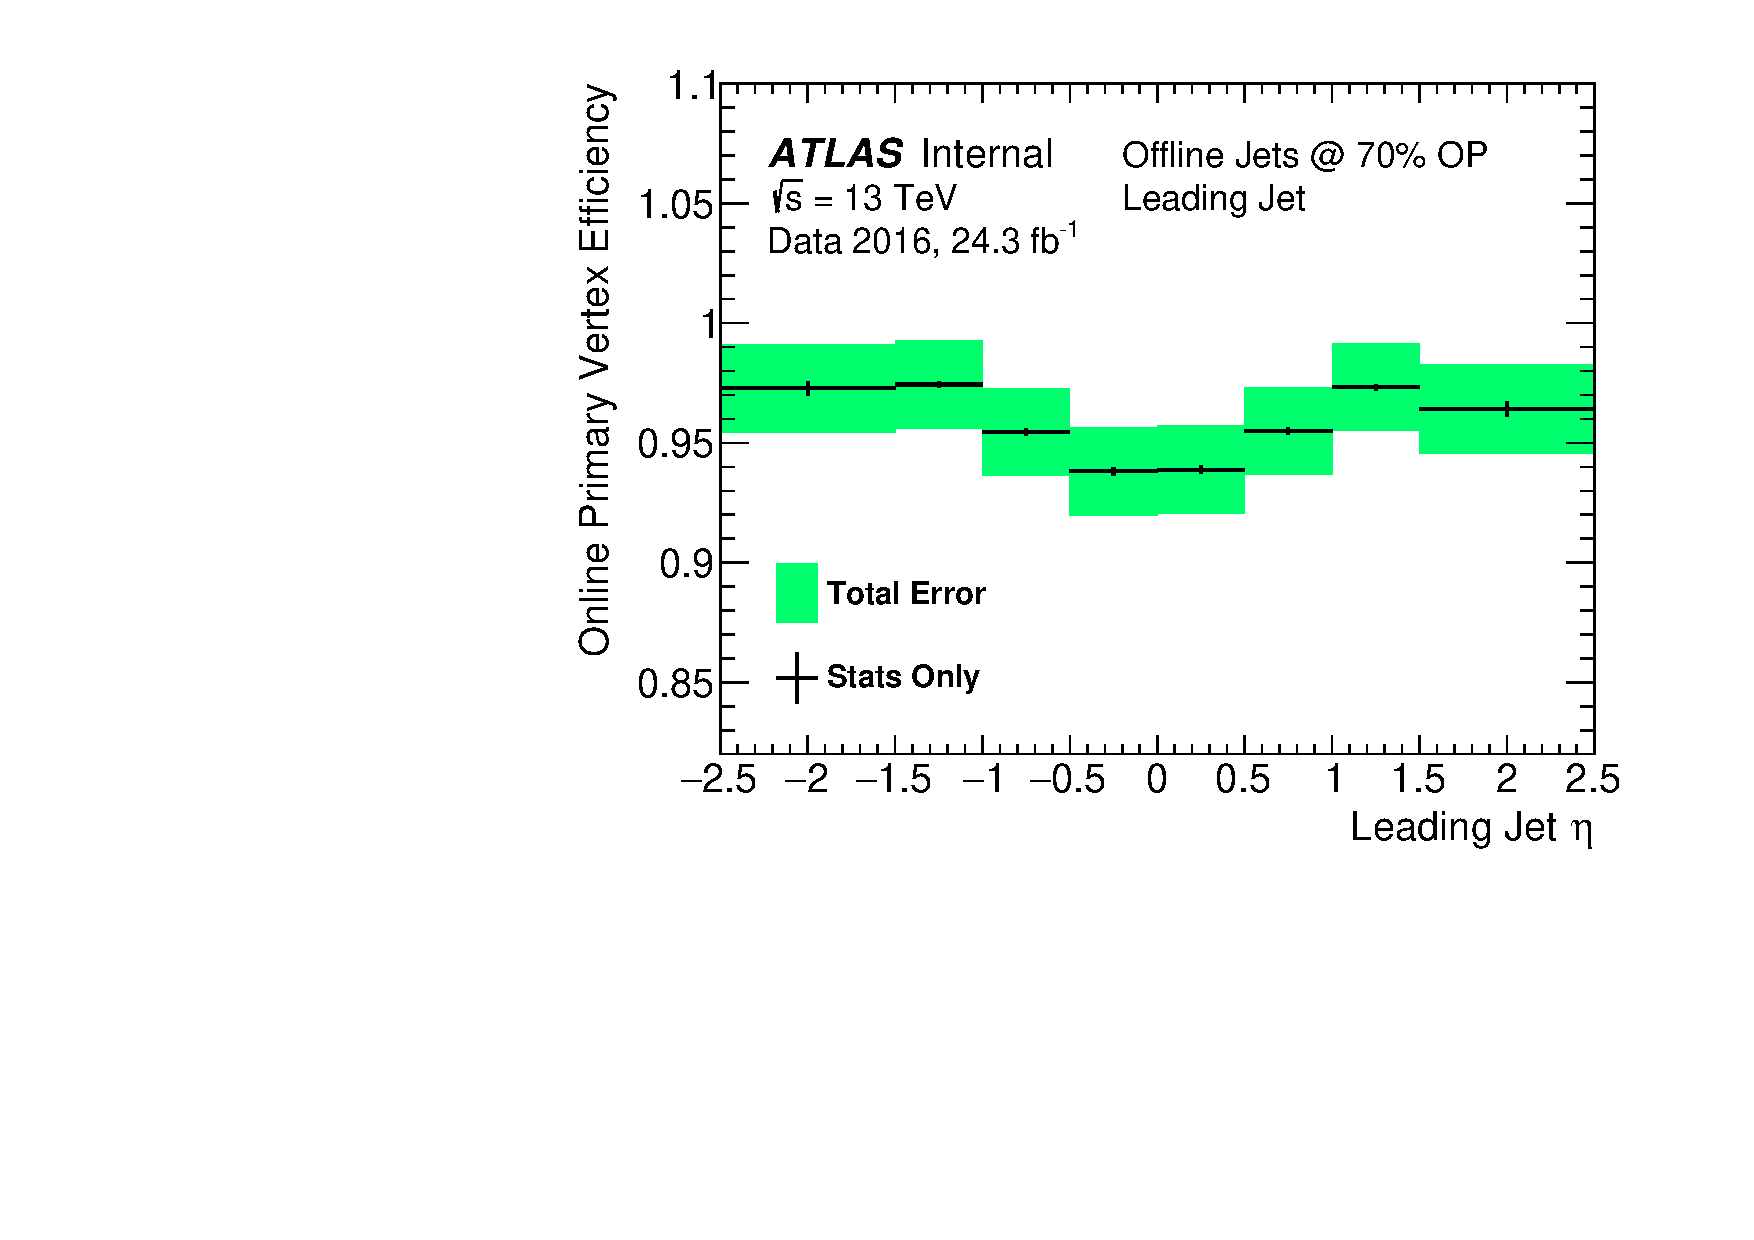
\includegraphics[width=0.8\linewidth, angle=0]{figs/Trigger/fullSyst_EventEfficiency_leadingJetEta.pdf}
  \end{center}
  \caption[The measured online primary vertex efficiency as a function of offline leading jet-$\eta$.]
          {
    The measured online primary vertex efficiency as a function of offline leading jet-$\eta$.
    The central values and statistical uncertainties are shown in black and the green bands represent the total uncertainty.}
    \label{fig:bTrig_eventSys}
    \vspace{-1em}
\end{figure}

\begin{table}[!ht]
  \begin{center}
  \begin{tabular}{|c||c|c||c|c|c||c|}
    \hline
\multirow{2}{*}{Leading Jet $\eta$} & Event-level  & Total       & \multicolumn{3}{c|}{Sources of Uncertainty} \\ \cline{4-6} 
                                    & Efficiency   & Uncertainty & Data Stat. & MC Stat. & Shape Syst. \\
\hline
-2.5--1.5 & 97.3\% & 1.9\% & 0.3\% & 0.1\% & 1.9\%  \\
-1.5--1.0 & 97.4\% & 1.9\% & 0.1\% & 0.0\% & 1.9\%  \\
-1.0--0.5 & 95.5\% & 1.9\% & 0.1\% & 0.0\% & 1.9\%  \\
-0.5-0.0  & 93.8\% & 1.9\% & 0.2\% & 0.0\% & 1.9\%  \\
0.0--0.5  & 93.9\% & 1.9\% & 0.2\% & 0.0\% & 1.9\%  \\
0.5--1.0  & 95.5\% & 1.9\% & 0.2\% & 0.0\% & 1.9\%  \\
1.0--1.5  & 97.3\% & 1.9\% & 0.1\% & 0.0\% & 1.9\%  \\
1.5--2.5  & 96.4\% & 1.9\% & 0.3\% & 0.1\% & 1.9\%  \\
\hline
\end{tabular}
  \caption{\label{tab:bTrig_eventEff} A table showing the event-level online primary vertex efficiency as a function of leading jet-$\eta$
    with total uncertainty and the contributions of the different systematic uncertainties considered.}
  \end{center}
\end{table}

\vfill

%\FloatBarrier
%
%\subsection{Cross-checks}
%\subsubsection{Simulation checks}
%- Ttbar alone vs ttbar+tW\\
%- Try powheg
%\subsubsection{Electron/Muon overlap checks}
%\subsubsection{Event Level Eff: Showing correlation with $z_{\,\text{bs}}^{\text{\,online}}$}
%- Show that it comes from high beamspot z-position only.\\
%- i.e. $\epsilon_{\text{PV}}$ vs eta for different bs regions.
%\subsubsection{Event Level Eff: Re-weighting of sub-leading jet}
%- We did a test where we applied correction to leading and showes the subleading was flat within systematic uncertainty (2%)
%
%Any others that are good?
%
%Cross-checks can be moved to appendix
%
%\section{To Do}
%
%These can be considered on my list.
%\noindent
%- Cite in plot caption\\
%- Update plots to most current version (and label those that are not)\\
%- In caption I want (a) befor plot i.e. (a) jet-pT, (b) jet-eta.
%- Always use data/simulation instead of data/simulation\\
%- use Epoch~instead of epoch\\
